%
%  Constructuve Alignment for Introductory Programming
%
%  Created by Andrew Cain on 2011-02-10.
%  Copyright (c) 2011 Swinburne University. All rights reserved.
%
\documentclass[12pt,a4paper,twoside]{report}

%!TEX root = Constructive Alignment for Introductory Programming.tex

% Essential packages
%\usepackage{times}
%\usepackage{helvet}



\usepackage{amsmath, amssymb, amsthm, amstext}
\usepackage[font=small, labelfont=bf, margin=20pt]{caption} 
\usepackage[pdftex]{graphicx}
\usepackage[left=40mm, right=25mm, top=33mm, bottom=33mm, headheight=14pt]{geometry}

\usepackage[authoryear]{natbib}
\bibliographystyle{agsm} %{abbrv}

\usepackage{subfig}
\usepackage{flushend}
\usepackage{rotating}
% \usepackage{array,longtable} breaks tables?
% \usepackage{tabulary}
\usepackage{multicol}
\usepackage{multirow}
\usepackage{setspace}
\usepackage{cite}
\usepackage{url}
\usepackage{enumitem}
\usepackage{pdflscape}

\usepackage{nameref}

\usepackage{pdfsync}

\renewcommand{\cite}{\citep}

\usepackage{tgbonum} %% Use the extended bookman font

% Optional customisation packages
\usepackage{mathpazo}
\usepackage{algorithm, algpseudocode}

% \usepackage[compact]{titlesec}
% \titlespacing{\section}{0pt}{16pt}{0pt}
% \titlespacing{\subsection}{0pt}{14pt}{0pt}
% \titlespacing{\subsubsection}{0pt}{12pt}{0pt}

% Page layout
\parindent 0pt
\parskip 0.20in
%\parskip 2.0ex
%\renewcommand{\baselinestretch}{1.5}
%\renewcommand{\baselinestretch}{1.33}
\numberwithin{equation}{section}
\renewcommand{\bibname}{References}
\renewcommand{\contentsname}{Contents}
%\pagenumbering{roman}
\footskip 70pt

%------------------------------------------------------------------------- %
% Stuff needed to use PDF figures inside this document
% \usepackage{times}
\usepackage{xspace}
% \usepackage{graphicx}
\graphicspath{{Figures/}}
%\usepackage[pdftex,colorlinks=true,pdfstartview=FitV,
%  linkcolor=black,citecolor=black,urlcolor=black]{hyperref}
%---------------------------------------------------------------------------% 
% Markup macros for proof-reading
\usepackage[normalem]{ulem} % for \sout
\usepackage{xcolor}
\newcommand{\ra}{$\rightarrow$}
\newcommand{\ugh}[1]{\textcolor{red}{\uwave{#1}}} % please rephrase
\newcommand{\ins}[1]{\textcolor{blue}{\uline{#1}}} % please insert
\newcommand{\del}[1]{\textcolor{red}{\sout{#1}}} % please delete
\newcommand{\chg}[2]{\textcolor{red}{\sout{#1}}{\ra}\textcolor{blue}{\uline{#2}}} % please change

%------------------------------------------------------------------------- %
% Put edit comments in a really ugly standout display
\usepackage{ifthen}
\usepackage{amssymb}
\newboolean{showcomments}
\setboolean{showcomments}{true} % TOGGLE true/false to show or hide comments
\ifthenelse{\boolean{showcomments}}
  {\newcommand{\note}[2]{
	\fbox{\bfseries\sffamily\scriptsize#1}
    {\sf\small$\blacktriangleright$\textit{#2}$\blacktriangleleft$}
   }
  }
  {\newcommand{\note}[2]{}
   \newcommand{\version}{}
  }
\newcommand{\here}{\note{***}{CONTINUE HERE}}
\newcommand\ml[1]{\note{ML}{#1}}
\newcommand\rv[1]{\note{RV}{#1}}
\newcommand\todo[1]{\note{TODO}{#1}}
\newcommand\review[1]{\note{REVIEW}{#1}}
\newcommand\jgs[1]{\note{JGS}{#1}}
\newcommand\pbr[1]{\note{PBRANCH}{#1}}
\newcommand{\msystems}{\emph{forty}}
\newcommand{\mversions}{1057}
\newcommand{\mchangedversions}{1017}  %% This will be mversions - msystems
\newcommand{\mclasses}{55000}

%-------------------------------------------------------------------------
\newcommand{\sref}[1]{Section~\ref{#1}}
\newcommand{\fref}[1]{Figure~\ref{#1}}
\newcommand{\cref}[1]{Chapter~\ref{#1}}
\newcommand{\aref}[1]{Appendix~\ref{#1}}
\newcommand{\tref}[1]{Table~\ref{#1}}
\newcommand{\eqnref}[1]{Equation~\ref{eqn:#1}}

\newcommand{\cnref}[1]{\nameref{cha:#1}}

%-------------------------------------------------------------------------
\newcommand{\bs}{\symbol{'134}} % backslash
\newcommand{\us}{\symbol{'137}} % underscore
\newcommand{\ie}{\emph{i.e.}\xspace}
\newcommand{\eg}{\emph{e.g.}\xspace}
\newcommand{\etal}{\emph{et al.}\xspace}
%-------------------------------------------------------------------------

\newcommand{\CA}{Constructive Alignment\xspace}
\newcommand{\IP}{Introductory Programming\xspace}
\newcommand{\OBTL}{Outcomes-Based Teaching and Learning\xspace}


%-------------------------------------------------------------------------

% Macros for type dependency graph section
\newcommand{\tg}{$G^T$}
\newcommand{\ind}[1]{$l_{in}({#1})$}
\newcommand{\outd}[1]{$l_{out}({#1})$}
\newcommand{\inid}[1]{$l^{i}_{in}({#1})$}
\newcommand{\ined}[1]{$l^{e}_{in}({#1})$}
\newcommand{\outid}[1]{$l^{i}_{out}({#1})$}
\newcommand{\outed}[1]{$l^{e}_{out}({#1})$}

\newcommand{\defeq}{\stackrel{\textrm{\scriptsize def}}=}
\newcommand{\edge}[2]{\langle{#1},{#2}\rangle}
\newcommand{\card}[1]{\mid\! #1 \!\mid}  %% Will only work in Math mode
%-------------------------------------------------------------------------
% % Metrics used
% \newcommand{\fanin}{In-Degree Count\xspace}
% \newcommand{\fanout}{Out-Degree Count\xspace}
% \newcommand{\indeg}{In-Degree\xspace}
% \newcommand{\outdeg}{Out-Degree\xspace}
% \newcommand{\WMC}{Weighted Method Count\xspace}
% \newcommand{\bc}{Branch Count\xspace}
% \newcommand{\fcount}{Field Count\xspace}
% \newcommand{\mcount}{Method Count\xspace}
% \newcommand{\icount}{Interface Count\xspace}
% \newcommand{\supcount}{Super Class Count\xspace}
% \newcommand{\paracount}{Parameter Count\xspace}
% \newcommand{\tycount}{Type Construction Count\xspace}

% \newcommand{\OSS}{Open Source Software}
% \newcommand{\OSYS}{Open Source Software Systems}
% \newcommand{\OO}{object oriented}


% % used metrics
% \newcommand{\Metric}[1]{\emph{#1} \emph{Count}}
% \newcommand{\Gini}{Gini Coefficient}
% \newcommand{\Ginis}{Gini Coefficients}

% \newcommand{\LIC}{\emph{Load Instruction Count}}
% \newcommand{\SIC}{\emph{Store Instruction Count}}
% \newcommand{\CC}{\emph{Number of Branches}}
% \newcommand{\NOB}{\emph{Number of Branches}}
% \newcommand{\IDC}{\emph{In-Degree Count}}
% \newcommand{\ODC}{\emph{Out-Degree Count}}
% \newcommand{\MC}{\emph{Number of Methods}}
% \newcommand{\NOM}{\emph{Number of Methods}}
% \newcommand{\PMC}{\emph{Public Method Count}}
% \newcommand{\NOF}{\emph{Number of Fields}}
% \newcommand{\NOA}{\emph{Number of Attributes}}
% \newcommand{\FC}{\emph{Number of Attributes}}
% \newcommand{\MIC}{\emph{Fan-Out Count}}
% \newcommand{\TCC}{\emph{Type Construction Count}}
% \newcommand{\NOD}{\emph{Number of Descendants}}
% \newcommand{\NOC}{\emph{Number of Children}}
% \newcommand{\DIT}{\emph{Depth of Inheritance Tree}}
% \newcommand{\MCC}{\emph{Fan-Out Count}}

% \newcommand{\LICs}{LIC}
% \newcommand{\SICs}{SIC}
% \newcommand{\CCs}{NOB}
% \newcommand{\IDCs}{IDC}
% \newcommand{\ODCs}{ODC}
% \newcommand{\MCs}{NOM}
% \newcommand{\PMCs}{PMC}
% \newcommand{\FCs}{NOA}
% \newcommand{\MICs}{FOC}
% \newcommand{\TCCs}{TCC}
% \newcommand{\NODs}{NOD}
% \newcommand{\NOCs}{NOC}
% \newcommand{\DITs}{DIT}
% \newcommand{\MCCs}{MCC}

% \newcommand{\GC}{\Metric{Getter}}
% \newcommand{\SC}{\Metric{Setter}}
% \newcommand{\BC}{\Metric{Boxing}}

% %% Additional commands to provide for commenting and notes
% \newcommand{\rb}[1]{\raisebox{1.5ex}[0pt]{#1}}
% \newcommand{\rbp}[1]{\raisebox{1.5ex}[0pt]{\parbox{7cm}{#1}}}
% \newcommand{\cl}{\\ \cline{3-4}}



%%%%%%%%%%%%%%%%%%%%%%%%%%%%%%%%%%%%%%%%%%%%%%%%%%%%%%%%%%%%%%%%%%%%%%%%%%%%%
% Customising chapter headings (optional) - see sectsty.pdf
%\usepackage{sectsty}
%\chapterfont{\large\sc\centering}
%\chaptertitlefont{\large\sc\centering}
%\subsubsectionfont{\small\sc\centering}
%\subsubsectionfont{\centering}


%---------------------------------------------------------------------------
% Customise header to show chapter - see fancyhdr.pdf
\usepackage{fancyhdr}
\pagestyle{fancy} % default ``plain''
\fancyhf{} % clear all rules
\rhead{} % default - chapter
\lhead{\nouppercase{\textsc{\leftmark}}} % default - section
\renewcommand{\headrulewidth}{0.4pt} % thin line
%\renewcommand{\footrulewidth}{0.4pt} % thin line
\makeatletter
%\renewcommand{\chaptermark}[1]{\markboth{\textsc{\@chapapp} \thechapter: #1}{}}
\renewcommand{\chaptermark}[1]{\markboth{\MakeUppercase{\chaptername \xspace \thechapter. #1}}{}}
\cfoot{} % remove the page number in the middle of footer
% \rfoot{\thepage}
\fancyfoot[R]{\thepage}
%\fancyhead[R]{\thepage}

%% The following commands force page numbers to right at start of new chapter
%% Needed because Latex will override fancy headers on first page of new chapters
\fancypagestyle{plain}{\fancyhf{} % clear all header and footer fields 
%\fancyhead[R]{\thepage}
%\renewcommand{\chaptermark}[1]{\markboth{\MakeUppercase{\chaptername \xspace \thechapter. #1}}{}}
%\renewcommand{\headrulewidth}{0.4pt} % thin line
\renewcommand{\headrulewidth}{0pt} 
\renewcommand{\footrulewidth}{0pt}
\fancyfoot[R]{\thepage}} % page number in centre

\makeatother

% Remove the Warning: \headheight is too small (12.0pt):
\setlength{\headheight}{15pt}



%-----------------------------------------------------------------------
% red and blue boxes for drafting notes
%-----------------------------------------------------------------------
\definecolor{boxgray}{gray}{0.9}

\newcommand{\mycolorbox}[3]{
 \vspace{5mm}
 \noindent
 \fcolorbox{#1}{#2}{
   \begin{minipage}[l]{0.95\textwidth}
     \color{#1}
     #3
   \end{minipage}
 }
 \vspace{3mm}
}

\newcommand{\myredbox}[1]{\mycolorbox{red}{boxgray}{#1}}
\newcommand{\mybluebox}[1]{\mycolorbox{blue}{boxgray}{#1}}
\newcommand{\mygreybox}[1]{\mycolorbox{black}{boxgray}{#1}}
\newcommand{\mywhitebox}[1]{\mycolorbox{black}{white}{#1}}



%\usepackage[pdftitle={title here},pdfpagemode=UseOutlines,
%colorlinks=true,pdfauthor={author here},pdfpagetransition=Dissolve,
%bookmarks=true,pdftex=true,plainpages=false,pdfpagelabels,backref]{hyperref}

%PDF hyper-linking (set colors to black for printing)
\usepackage[colorlinks]{hyperref}
\hypersetup{colorlinks,
	linkcolor=black,
	filecolor=black,
	urlcolor=black,
	citecolor=black}


%\usepackage[ps2pdf=true,colorlinks]{hyperref}
%\usepackage[figure,table]{hypcap}
%\hypersetup{
%	bookmarksnumbered,
%	pdfstartview={FitH},
%	citecolor={blue},
%	linkcolor={red},
%	urlcolor={black},
%	pdfpagemode={UseOutlines}
%}
%\makeatletter
%\newcommand\org@hypertarget{}
%\let\org@hypertarget\hypertarget
%\renewcommand\hypertarget[2]{%
%  \Hy@raisedlink{\org@hypertarget{#1}{}}#2%
%} 
%\makeatother 

%\usepackage[T1]{fontenc}
%\usepackage{lmodern}
%\usepackage{times}
%\usepackage{bookman}
%% Use the extended bookman font
%\usepackage{tgbonum}
%\usepackage{cmbright}

%\usepackage{fontspec} 

% DOCUMENT LAYOUT
%\usepackage{geometry} 
%\geometry{a4paper, textwidth=5.5in, textheight=8.5in, marginparsep=7pt, marginparwidth=.6in}
%\setlength\parindent{0in}

% FONTS
% converts LaTeX specials (``quotes'' --- dashes etc.) to unicode
%\defaultfontfeatures{Mapping=tex-text} 
%\setromanfont [Ligatures={Common}, Numbers={OldStyle}]{Hoefler Text}
%\setmonofont{Monaco} 
%\setsansfont{Optima Regular}
%\setromanfont{Optima}

%\setmonofont[Scale=0.9]{Monaco} 
%\setsansfont[Scale=0.9]{Optima Regular}
%\setromanfont{Optima}

\usepackage{listings}
\usepackage{color}
% \usepackage{textcomp}

%\definecolor{listinggray}{gray}{0.9}
%\definecolor{lbcolor}{rgb}{0.9,0.9,0.9}

\lstset{
    %float=p,
    %floatplacement=p,
    %boxpos=t,
%	backgroundcolor=\color{lbcolor},
	tabsize=2,
%	rulecolor=,
	language=Java,
    basicstyle=\scriptsize,
    %basicstyle=\footnotesize,
    upquote=true,
    aboveskip={\bigskipamount},
	belowskip={\medskipamount},
	lineskip={\smallskipamount},
    columns=fixed,
    showstringspaces=false,
    breaklines=true,
	numbers=left,
	captionpos=b,
	abovecaptionskip={\bigskipamount},
	belowcaptionskip={\medskipamount},
%    prebreak = \raisebox{0ex}[0ex][0ex]{\ensuremath{\hookleftarrow}},
    frame=single,
    identifierstyle=\ttfamily,
    keywordstyle=\color[rgb]{0,0,1},
    commentstyle=\color[rgb]{0.133,0.545,0.133}\bfseries,
    stringstyle=\color[rgb]{0.627,0.126,0.941}
%	stringstyle=\ttfamily
}


\ifpdf
\DeclareGraphicsExtensions{.pdf, .jpg, .tif}
\else
\DeclareGraphicsExtensions{.eps, .jpg}
\fi

\usepackage{phdthesis}

\includeonly{03-Principles}


% Use utf-8 encoding for foreign characters
\usepackage[utf8]{inputenc}

% % Setup for fullpage use
% \usepackage{fullpage}
%


% % Uncomment some of the following if you use the features
% %
% % Running Headers and footers
% %\usepackage{fancyhdr}
% 
% % Multipart figures
% %\usepackage{subfigure}
% 
% % More symbols
% %\usepackage{amsmath}
% %\usepackage{amssymb}
% %\usepackage{latexsym}
% 
% % Surround parts of graphics with box
% \usepackage{boxedminipage}
% 
% % Package for including code in the document
% \usepackage{listings}
% 
% % If you want to generate a toc for each chapter (use with book)
% \usepackage{minitoc}
% 

\onehalfspacing

\begin{document}

\title{Constructive Alignment for Introductory Programming}
\author{Andrew Cain}

\date{2011-02-10}

\maketitle

\chapter{Introduction} % (fold)
\label{cha:introduction}

% Context, general problem, current solutions, why these solutions are still lacking, broadly what needs to be solved, my focus and research goal (something like that)
Programming is a critical skill in Computer Science and Software Engineering, as a consequence students in these fields are taught programming from the start of their degree programmes at many Universities. Although we have been teaching programming for a number of decades, learning programming remains challenging for many students \cite{Jenkins:2002,Lister:2004,McCracken:2001,Ragonis:2007,Robins:2003,Rountree:2002,Renumol:2010,Wiedenbeck:2005}, with a general consensus that many students find programming hard. 

Despite persistent efforts over many years, we are still a long way from having specific guidance on how best to approach teaching introductory programming. Attempts in the field of computing education research have focused on curriculum, pedagogy, language choice, and tool support \cite{Pears:2007}. Further afield, advancements from general education literature provides additional advice on underlying theories and practices, including works on the scholarship of teaching and learning \cite{Boyer:1990}, approaches to teaching \cite{Martin:2000}, approaches to learning \cite{Marton:1976a,Trigwell:1999}, and analysis of the learner's experience \cite{Marton:1997}. 

While seen as beneficial, these general education theories are seen as distant from the teaching of introductory programming, and there is a need for a greater inclusion of these topics in the computing education research discourse to help engage academics teaching \IP.

In their study of students' experiences learning to program, \citet{Bruce:2003} categorised the way students engage with learning to program into five categories range from approaches focusing on ``\emph{getting through the unit}'', to approaches aimed at discovering what it means to be a programmer. Each of these categories can be broadly classified as either a surface or deep approach \cite{Marton:1976a,Ramsden:1992} to learning to program. When engaging surface approaches, students attempt to address the outcomes with as little effort as possible. This leads to situations in which students are primarily motivated by fear of failing, and experience the learning as a struggle, with the topic appearing tedious, hard and boring. Adjectives that are often associated with learning to program. On the other hand, when engaging deep approaches to learning students seek meaning in what they do, and relate their learning to the bigger picture. To succeed at learning to program, students need to engage deep approaches to learning, as surface approaches alone are unlikely to be sufficient \cite{Bruce:2003}.

Biggs' model of \CA \cite{Biggs:1996c,Biggs:2007}, based upon constructive learning theory (constructivism) and aligned curriculum \cite{Cohen:1987}, aims to enhance student learning outcomes by focusing on \emph{what the student does}, encouraging students to use \emph{deep}, rather than \emph{surface}, approaches to learning. As a form of outcomes based teaching and learning, \CA involves defining intended learning outcomes using verbs that indicate the required cognitive level students must engage. Students' work can then be assessed by evaluating the structure of the observed learning outcome, using the SOLO Taxonomy developed by \citet{Biggs:1982}. While there is extensive literature on \CA in the general education literature, it has received little attention in computing eduction research related to teaching introductory programming. 

\todo{ In this thesis }

% - image on iterative nature of teaching

% Research Questions and Method

% Key Findings - page

% Thesis Structure - para for each chapter

This work will look to answer the following question. In what way can \emph{constructive alignment} be applied to the teaching of \emph{introductory programming} to stimulate \emph{deep approaches learning}?

To answer this question it is necessary to design and implement an introductory programming subject using the principles of constructive alignment. Designing such a subject requires the definition of intended learning outcomes, a statement of the assessment criteria, aligned teaching and learning activities, and a specific assessment approach. These activities require the following questions to be asked.

\begin{enumerate}
  \item What are appropriate intended learning outcomes?
  \item Given the stated learning objectives, how can assessment criteria be structured to encourage students to use progressively deeper cognitive levels of activity in order to achieve higher grades? (memorise to reflect)
  \item What teaching and learning activities help create an effective learning environment that encourages deep approaches to learning and a meaningful student experience?
  \item How can criterion referenced assessment and holistic grading be used to assess student outcomes?
\end{enumerate}

To assess the effectiveness of the proposed teaching method the following questions will be addressed.

\begin{enumerate}
  \item Does this teaching method change the way students approach learning and/or their work in general?
  \item What affect does this teaching method have on student engagement?
  \item Are students able to effectively select material to demonstrate coverage of the intended learning outcomes?
  \item To what depth does submitted work demonstrate the intended learning outcomes?
  \item To what degree are students able to correctly assess their work against the subject's assessment criteria?
  \item How well do students retain the knowledge and skills they develop in the subject?
\end{enumerate}

% Improve depth of learning.
% 
% Our method of teaching with constructive alignment: 
% \begin{itemize}
%   \item Determine learning objectives
%   \item Create tiered assessment criterion that provide requirements for differing depths of understanding...
%   \item Make students responsible for as much of their learning as possible. It is what they do that counts.
%   \item Teach programming, not the language. Focus lectures on concepts and abstractions, provide just enough syntax to get the students started.
%   \item Provide resources for students to learn the required syntax to map concepts to code (podcasts, text) to allow them to learn independently.
%   \item Provide regular formative feedback on assessment work
%   \item Have students prepare a portfolio of their work that demonstrates how they have addressed the assessment criteria
% \end{itemize}
% 
% \bigskip
% 
% Guiding principles:
% \begin{itemize}
%   \item Truth. Remain true to the language and how it should be used. Avoid half truths as much as possible.
%   \item Trust. Students are there to learn. They are capable and just need direction, encouragement, and feedback. Theory Y.
%   \item Construct knowledge. Introduce the concepts needed to fully\footnote{Fully at this level of abstraction.} understand the programs they are writing. Avoid all forms of `magic'.
%   % \item Students should use deep approaches to learning.
%   % \item Programs are not sufficient to assess the depth of a students understanding.
%   \item Maintain a good signal to noise ratio. Provide the essential material and have students explore the details themselves.
%   \item Encourage deep exploration once concepts are grasped. For example, encourage students to look at how programming mechanisms work like how parameter passing works, how the stack grows, how a program's memory is organised.
%   \item Flexible delivery with clear learning outcomes that allow students to customise the learning experience to their own needs and interests.
%   \item Self efficacy allowing students to work toward a grade.
% \end{itemize}
% 
% \clearpage

% In what way can \emph{constructive alignment} be applied to the teaching of \emph{introductory programming} to stimulate \emph{deep learning}?

% (Breadth vs depth)
% 
% What are the benefits of \emph{constructive alignment} for the teaching of \emph{introductory programming}?
% 
% What is the impact of \emph{constructive alignment} on overall computer science curriculum?
% 
% Does \emph{constructive alignment} encourage \emph{deep approaches to learning} in introductory programming subjects?




% \begin{enumerate}
%   \item How have other educational areas implemented constructive alignment?
%   
%   \item What are appropriate learning objectives for an introductory programming subject?
%   \begin{itemize}
%     \item What are the related programming concepts and abstractions?
%     \item Are there established models of these concepts and abstractions?
%     \item How do the concepts and abstractions map to different programming paradigms and languages?
%     \item Which of these concepts and abstractions are appropriate for introductory programming subjects? What are the differences for subjects that use an `Objects First' approach versus an `Objects Later' approach? How do the two approaches compare on concept and abstraction coverage?
%   \end{itemize}
%   
%   \item Given the selected learning objectives, how can assessment criteria be structured to encourage students to demonstrate use of progressively deeper cognitive levels in order to achieve higher grades? (memorise to reflect)
%   \begin{itemize}
%       \item What are the different cognitive levels of activities related to programming? (Is programming really `application' or just `expression'? e.g. getting it to work does even mean the student can explain why/how it works.) How do these relate to deep and surface approaches? How does this map to the SOLO taxonomy. (Is there work related to this?)
%     % \item Can tiered assessment criteria be developed to map student outcomes to grade categories for use in criterion referenced assessment? How can these be formulated to encourage students to engage deeper learning approaches for higher grades?
%     \item Are students aware of what is required to achieve different grades, and how does this change during the semester?
%     \item What affect does the tiered assessment criteria and criterion referenced assessment have on student approaches to learning?
%     \item Do students use criterion referenced assessment to customise the learning experience to their own requirements,  interests, and aspirations?
%     \item Does this self directed learning and self efficacy help motivate students? Does this in turn lead to deeper approaches to learning and deeper learning outcomes?
%     \item How do student aspirations change as the semester progresses? 
%   \end{itemize}
%   
%   % \item What teaching and learning activities can help support the students to studying sound combination of theory and practice.
%   % \item What benefits are there from providing flexible teaching and learning activities that align with the selected learning outcomes?
%   % \item Given the selected learning outcomes, what are the benefits of providing flexible teaching and learning activities?
%   % \item What teaching and learning activities that support and motivate
%   % 
%   % \item What teaching and learning activities help support student self-directed leaning of the conten
%   % 
%   % \item Can innovative teaching and learning activities encourage students to use deep approaches to learning?
%   % 
%   % \item Given the learning objective and assessment criteria, what teaching and learning activities are effective/ineffective?
%   % 
%   % \item What do students find useful about the teaching and learning activities used?
%   
%   % \item What teaching and learning activities can create an effective learning environment and a meaningful student experience?
%   
%   \item What teaching and learning activities help create an effective learning environment and meaningful student experience?
%   \begin{enumerate}
%     \item How can we make more effective use of lecture time? 
%     \item Can we focus on programming concepts and abstractions at a higher level and use other means to cover details of language syntax?
%     \item Can language syntax be covered sufficiently if the lecture focus shifts toward concepts?
%     \item What effect does this have on student learning outcomes, sense of achievement, and learning approach?
%     \item Are video podcasts an effective means of demonstrating programming abstractions and syntax?
%     \item Does the focus on concepts help students learn a second programming language? How?
%     \item How much overhead is there in switching between languages?
%     \item Can you effectively teach programming using multiple languages in the one subject? What are the advantages and disadvantages of this?
%     \item How does covering multiple languages impact on the student's learning experience?
%     
%     \item Will students use a focused episodic text? (??)
%     % \item Motivation (Dan Pink, Motivation)
%     \item Self determination (efficacy)
%   \end{enumerate}
%   
%   % Holistic, 
%   % Formative assessment during the semester
%   
%   \item How can criterion referenced assessment and holistic grading be used as assess student outcomes in introductory programming subjects?
%   % \item Can portfolio assessment be used effectively for assessing student outcomes in introductory programming subjects?
%   \begin{enumerate}
%     \item What benefits are there from this approach to assessment and grading?
%     \begin{itemize}
%       \item Self efficacy?
%       \item Deep learning outcomes?
%     \end{itemize}
%     \item What mechanisms can be introduced to limit plagiarism?
%     \item Does the use of ungraded formative assessment during semester reduce plagiarism?
%     \item Are students able to grasp the 
%     \item What strategies work effectively for providing frequent formative feedback for large classes?
%     \item What about the portfolio assessment approach encourages or discourages plagiarism? What mechanisms can be put in place to further discourage plagiarism?
%     
%     \item How are student portfolios affected by the statement of the assessment criteria?
%     \item Does criterion referenced assessment alter the way students approach study in the subject?
%     \item Does criterion referenced assessment alter the way students approach study in other subjects?
%     \item Does their approach to portfolio assessment change in subsequent subjects that use the same approach? How? How do these changes (if there are any) relate to deep approaches to learning?
%     \item Can portfolio assessment be scaled to larger class sizes?
%   \end{enumerate}
%   
%   \item How do student approaches to learning change over time?
%   \begin{enumerate}
%     \item During the semester
%     \item Over the year
%     \item Across the course
%     \item After uni
%   \end{enumerate}
%   
%   \item What makes this an effective or ineffective method of teaching introductory programming?
%   \item What effect does this teaching method have on student graduate attributes? (communication, problem solving, etc.)
%   
% \end{enumerate}
% 
% Objective:
% \begin{enumerate}
%   \item Model of programming concepts and abstractions, with multiple views for different language and paradigms.
%   \item Guidelines on programming concepts applicable for introductory programming.
%   \item Guidelines for building tiered assessment criteria.
%   \item Guidelines, support for, benefits of constructive alignments etc.
%   \item Behaviour tree for diagnostic view when students incorrectly self assess their grade - what was the cause. Student incorrectly self assessed -> over/under -> etc. Vs our expectations vs assessment criteria (grade)
% \end{enumerate}

% chapter introduction (end)


%!TEX root = Constructive Alignment for Introductory Programming.tex

\chapter{Approaches to Constructive Alignment} % (fold)
\label{cha:background}

\section{Constructive Alignment} % (fold)
\label{sec:constructive_alignment}

\subsection{Constructivism} % (fold)
\label{sub:constructivism}

In designing teaching and learning contexts, educators use some form of theory of teaching and learning to guide their decision making.

theory of teaching and learning

espoused theory \cite{Argyris:1976}

\emph{objectivist}

\emph{constructivism} and \emph{phenomenography}


\cite{Cunningham:1996} 




\cite{Montessori:1946}

Constructivism is a theory of knowledge that focuses on the active role of the learner in constructing their own understanding. Dating back to \citet{Piaget:1950} constructivism exists in several forms: cognitive, individual, postmodern, radical and social constructivism \cite{Phillips:1995,Steffe:1995}. Each of these forms of constructivism has various implications for teaching and learning.









In his original paper on constructive alignment \citet{Biggs:1996c} adopted constructivism as a framework to help guide decision making in all facets of teaching and learning. Constructivism was chosen over phenomenography 

practical concerns


For this work we are interested in adapting \emph{constructive learning theories}

 taking practical aspects from constructivism in general and focusing on what the student does, as suggested by .


In proposing constructive alignment, 

Disconnect between theory in use and espoused theory: \cite{Phillips:2005}


Engage with and expand experience \cite{Dewey:1960} exploration, thinking and reflection

% subsection constructivism (end)

\subsection{Aligned Curriculum} % (fold)
\label{sub:aligned_curriculum}

% subsection aligned_curriculum (end)

\subsection{Reported Applications of Constructive Alignment} % (fold)
\label{sub:reported_applications_of_constructive_alignment}

% subsection reported_applications_of_constructive_alignment (end)

% section constructive_alignment (end)

\section{Portfolio Assessment} % (fold)
\label{sec:portfolio_assessment}

% section portfolio_assessment (end)




% chapter background (end)
% %!TEX root = Constructive Alignment for Introductory Programming.tex

\chapter{Research Design and Ethics} % (fold)
\label{cha:research_design_and_ethics}

% chapter research_design_and_ethics (end)
%!TEX root = Constructive Alignment for Introductory Programming.tex

\chapter{Guiding Principles} % (fold)
\label{cha:guiding_principles}

\graphicspath{{Figures/CAApproach/}}

%
% JG - this is great!
%

This chapter describes twelve principles that underlie our model for delivering constructive aligned introductory programming. These principles act as guidelines for decision making, and in many ways underpin the model in the same manner as a unit's intended learning outcomes underpin constructively aligned teaching. Each aspect of the model, the associated curriculum, teaching and learning activities, and assessment tasks are aligned with one or more of these principles. 

The principles cover both \emph{how} the teaching and learning environment should operate, and \emph{what} should be taught. Originally derived from constructive alignment, the \emph{how} principles centre on constructivism and aligned curriculum. In relation to \emph{what} should be taught, the principles draw upon computing education literature and our own experiences as educators and software developers. 

Reflective practice played an important part in the formation of these principles, and both sets of principles have developed over the course of this research. This chapter presents the current working principles we use to guide the development and delivery of introductory programming. While most were present throughout the research, their individual emphasis and relationships have developed through our reflective practice. 

%
% JG - I wondered about expanding this to give a bit more overview about what is in each main section??
% AC - Done

The chapter first outlines the principles related to \emph{how} we aim to teach introductory programming, in \sref{sub:principles_for_how_the_environment_should_operate}. These principles relate to the core principles of constructive alignment, described in \cref{cha:background}, but also aim to more tightly integrate constructivist theories, with their strongly student-centred focus. Following this, \sref{sec:principles_to_guide_what_we_should_cover} presents the principles related to \emph{what} we aim to teach, specifically covering details on what we aim to focus on in teaching introductory programming. The full set of principles is this summarised in \sref{sec:summary_of_guiding_principles}.

\clearpage


\section{Princiles to guide HOW we should teach} % (fold)
\label{sub:principles_for_how_the_environment_should_operate}

Interventions that impact on the learning environment, also referred to as the teaching or academic environment, have been shown to have the potential to positively influence student learning outcomes \cite{Trigwell:1991}. Learning environments have also been found to influence students' approach to learning \cite{Entwistle:1990,Entwistle:1991,Kember:2007} and perceptions of teaching environments have been shown to directly, and indirectly, influence learning outcomes \cite{Meyer:1990,Lizzio:2002}. The aim of these first principles is therefore to create a positive learning environment for students; one that is demanding of students but supports and rewards their efforts to understand the concepts required of the curriculum. 

The following list outlines these principles for educators:
\begin{description}[noitemsep,nolistsep]
	\item [\Pref{itm:construct}]: Recognise that students construct knowledge in response to activity.
	\item [\Pref{itm:align}]: Align activities and assessment to intended learning outcomes.
	\item [\Pref{itm:formative}]: Assess learning outcomes, not learning pace or product outcomes. 
	\item [\Pref{itm:focus}]: Focus on important aspects, while providing access to necessary details.
	\item [\Pref{itm:expectations}]: Communicate high expectations.
	\item [\Pref{itm:support}]: Actively support student efforts.
	\item [\Pref{itm:theory_y}]: Trust and empower students to manage their own learning.
	\item [\Pref{itm:agile}]: Be agile and willing to change in response to measurable indicators.
	\item [\Pref{itm:reflect}]: Embed reflective practice in all aspects.
\end{description}

These first nine principles relate to \emph{how} the teaching and learning environment should operate and could, therefore, be applied to a range of teaching and learning contexts and topic domains.

Individually each principle has its own merits but they are designed to work together. As a whole, each principle interacts with the other principles to create a productive student-centred learning environment. \fref{fig:how_principles} shows the key interactions between these principles. The students active construction of knowledge is central, with various aspects of this being supported by the other principles. Each principle is discussed in detail in the following sections, with the various relationships being discussed along with associated literature.

\begin{figure}[htbp]
	\centering
	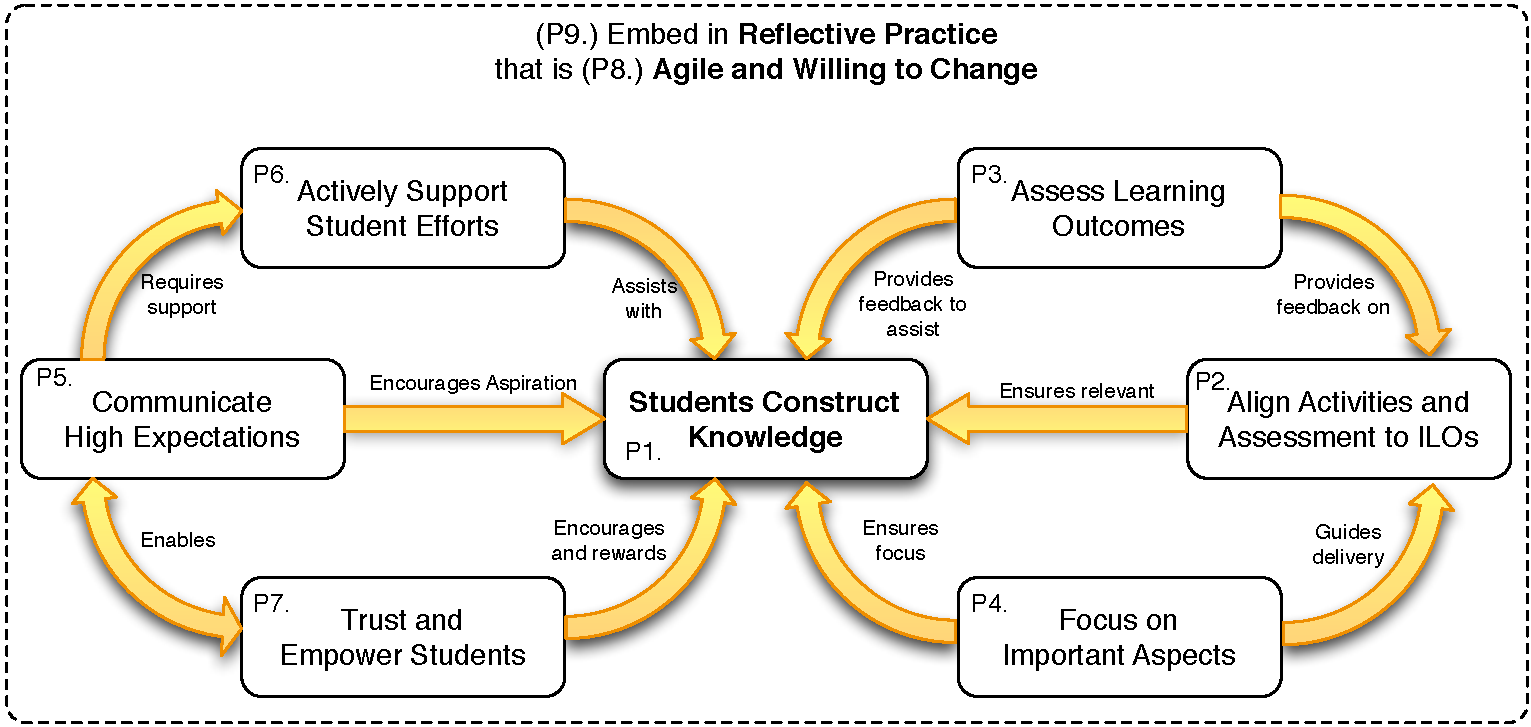
\includegraphics[width=\textwidth]{HowPrinciples}
	\caption{Key interactions between proposed principles for educators}
	\label{fig:how_principles}
\end{figure}


% section relationships_between_principles (end)
\subsection{Recognise students construct knowledge in response to activity} % (fold)
\label{ssub:ideas_adopted_from_constructivism}

Decisions about curriculum, teaching and learning activities, and assessment tasks are all guided by the educator's theory of teaching and learning \cite{Argyris:1976,Ramsden:1992}. While constructivism is often promoted by educators, \citet{Phillips:2005} observed that constructive learning theories have not transitioned to common education practice, resulting in a ``dissonance'' between the elements of effective learning and the characteristics of typical university learning environments. This is symptomatic of the disconnect between educators espoused theory and their theory-in-use \cite{Argyris:1976}. To successfully implement constructive alignment it is, therefore, important to identify and adopt the key aspects from constructivism, as outlined by \citet{Biggs:1996c}, \citet{Biggs:1997} and in \citet{Biggs:2007}. By adopting constructivism as our theory-in-use we aimed to create an educational setting that was ``in harmony'' with the principles of constructive alignment.

%
% JG - could add appropriate citations for source of each of these, if different
%

Central to all forms of constructivism is the principle that learning is an \emph{active process} requiring the leaner to construct their own understanding through individual and social activity \cite{Biggs:1996c,Cobb:1994,Duffy:1996,Duffy:1992,Glasersfeld:1989,Jonassen:1991,Steffe:1995,Vrasidas:2000}. To incorporate central ideas from these writings on constructive learning theories the following aspects of constructivism are actively embedded in the model presented in the next chapter:

\begin{itemize}[noitemsep,nolistsep]
	\item Knowledge is constructed, not transmitted via communication alone.
	\item Teaching involves creating a context in which learners are able to construct appropriate cognitive models through individual and social activities.
	\item Errors in understanding are opportunities for further learning, as these help indicate the students' current level of development and can be used to guide future learning activities.
\end{itemize}

\citet{Biggs:1996c} reason for adopting constructivism as a central philosophy was due to its emphasis on the students active role in constructing their own knowledge. When taken to an extreme this can result in approaches that rely upon students building their own understanding from ``first'' principles, possibly isolated concepts and without structure. Such approaches are promoted in discovery learning \cite{Bruner:1961} and in some constructivist writings, such as in \citet{Glasersfeld:1989} and \citet{Duffy:1996}. The unstructured nature of these teaching and learning environments have received strong criticism. 

\citet{Anderson:1998} criticises constructive learning theories when ``pursued to unproductive extremes'', as in the case with discovery learning, and argue that there is significant evidence of the benefits for guided instruction from the area of cognitive psychology. \citet{Mayer:2004} also argues against discovery learning, instead suggesting that constructivist views of education may be better served through cognitive activity, instructional guidance, and curricular focus. Furthermore, \citet{Kirschner:2006} argue against discovery learning, indicating that in highly complex environments, such as software development and introductory programming, free exploration may generate a heavy workload and detrimentally affect learning. 

%
% JG -  this reads a tad forward referencing to "the model" - could rephrase/retense to present e.g.
% "requires"  and "This approach will temper..."
%
% Presumabely many of these principles could be applied to produce a different model?
% 
% AC - Done
%

Embedding constructivism in the model proposed in this research required accepting the central role of the learner in constructing their knowledge, while avoiding detrimental aspects associated with taking these ideas to their extreme. This approach will temper constructivism with certain practical details, an approach we feel is in line with the principles of constructive alignment as originally proposed by \citet{Biggs:1996c}. These details include the following:

\begin{itemize}[noitemsep,nolistsep]
	\item Communication remains a valuable tool for educators to help shape the learning context, but should not be seen as a means of knowledge transfer.
	\item Guided instruction is valuable and ensures student activity is likely to be productive, though students should also have opportunities to explore content in a context meaningful to them individually.
	\item Deliberate practice provides students with opportunities to engage with principles in action, but these activities should include opportunities to reflect on important aspects learnt.
\end{itemize}

% section ideas_adopted_from_constructivism (end)

\subsection{Align activities and assessment to intended learning outcomes} % (fold)
\label{ssub:align_activities_and_assessment_to_intended_learning_outcomes_}

In order to implement constructive alignment we need to work iteratively toward achieving a ``web of consistency'' \cite{Biggs:1999} in which we optimise the likelihood of students \emph{engaging appropriately} with learning activities and assessment tasks. \cite{Biggs:1996c} indicates that this can be achieved through aligning learning activities and assessment tasks to the unit's intended learning outcomes. 

The alignment of activities and assessment to intended learning outcomes is critical for our model. As shown in \fref{fig:how_principles}, this alignment is seen as supporting student construction of knowledge. By aligning teaching and learning activities to the intended learning outcomes we ensure that students are constructing the required understanding. Similarly, by aligning assessment with these same intended learning outcomes we ensure that students are adequately prepared for this assessment and that the assessment is evaluating students' attainment of the stated learning outcomes. 

One potential issue identified in \cref{cha:background} is relying too heavily on staff to perform this alignment. This has the effect of placing the intended learning outcomes outside the process, interacted with only by staff when reporting their alignment to activities and assessment. This was shown visually in \fref{fig:misalignment}, with the students always two steps from the intended learning outcomes, which provided additional opportunities for misalignment.

\begin{figure}[htbp]
	\centering
	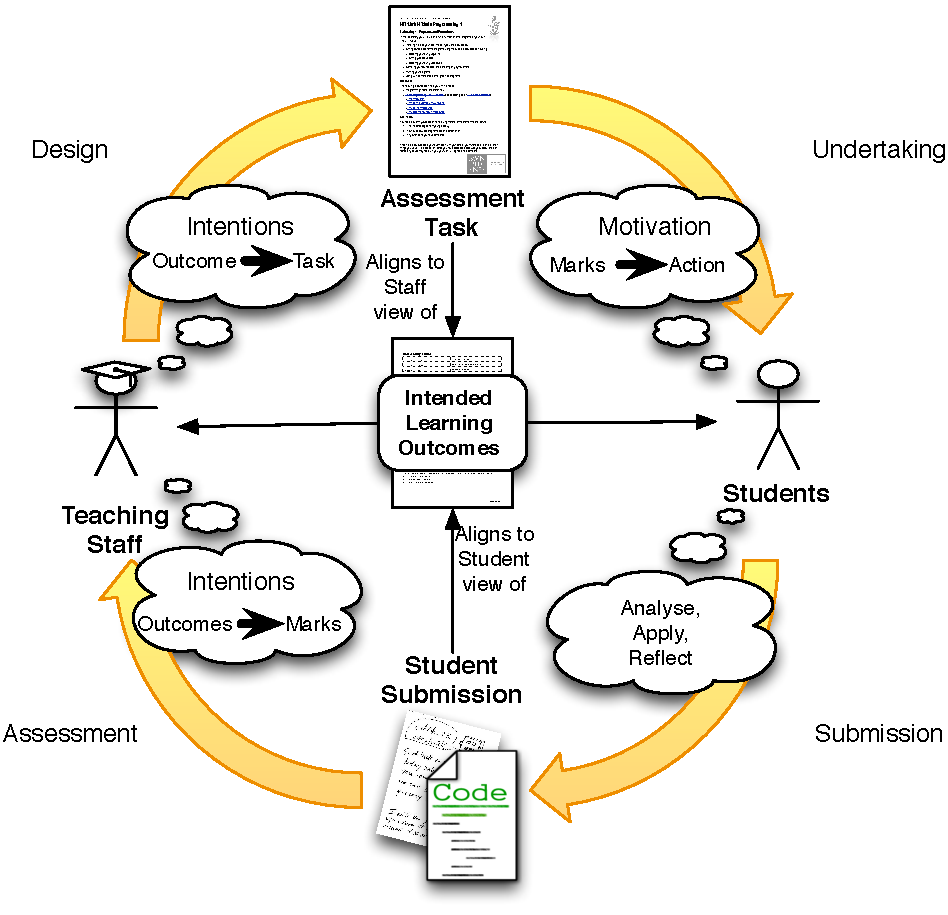
\includegraphics[width=\textwidth]{Alignment}
	\caption{An altered version of \fref{fig:misalignment} with students and staff now actively involved in aligning work to the unit's intended learning outcomes}
	\label{fig:alignment}
\end{figure}

\fref{fig:alignment} presents an altered version of \fref{fig:misalignment} from \cref{cha:background}. This illustrates how the intended learning outcomes become central to this process when students are included in the alignment process. The central role of the intended learning outcomes reduces the opportunities for misalignment, as now they form a central aspect shared by both staff and students. Staff and students now need to develop a shared understanding of the intended learning outcomes, and collaboratively work toward students being able to demonstrate they have met all outcomes. In this way, it should be possible to achieve the ``web of consistency'', and hopefully thereby improve the chances that students engage appropriately with learning activities and assessment tasks. 

% subsection align_activities_and_assessment_to_intended_learning_outcomes_ (end)


\subsection{Assess learning outcomes, not learning pace or product outcomes} % (fold)
\label{ssub:aim_to_assess_learning_outcomes_not_learning_pace_or_product_outcomes_}

Assessment in education is often seen as serving one of two possible purposes: supporting learning, or evaluating outcomes. These two purposes are known as \emph{formative assessment} and \emph{summative assessment}, as proposed by \citet{Scriven:1967} and \citet{Bloom:1969}. Formative assessment aims to assess student learning for the purpose of providing \emph{feedback}. This is distinct from summative assessment where the aim is to assess how well students have performed on a certain task, typically to determine a final \emph{grade}. \citet{Biggs:2007} suggest that for clarity the two forms of assessment are best referred to as \emph{formative feedback} and \emph{summative grading}.

The important role of formative feedback in education is widely reported. \citet{Ramsden:1992} indicates that, of all items on the Course Evaluation Questionnaire \cite{Ramsden:1991}, the one that most clearly distinguished between the best and worst courses related to the provision of helpful feedback. \citet{William:2006} described the use of formative feedback in short, medium and long cycles to improve student learning, and indicated that -- to be formative -- outcomes of the assessment must be used by students to make adjustments to better meet their learning needs. \citet{Black:1998} showed that substantial learning gains can be achieved by innovations designed to strengthen frequent feedback students receive. Furthermore, \citet{Black:1998} report that students pay more careful attention to feedback when there are no associated marks, or put another way ``marks'' reduced student attention to formative feedback. In discussing assessment for learning \citet{Brown:2004} stated that ``Formative feedback is critical'' and that ``feedback must be at the heart of the process'' if we are to make assessment an integral part of learning. 

\citet{Gibbs:2004} listed ten conditions under which assessment assists with student learning. These ten conditions can be grouped into three main point, as shown in the following list.

%
% JG - are these all in your own language/paraphrased - if so, good.  If not, reword :-)
% AC - done - reworded "ten" points... summary ours :)

\begin{itemize}[noitemsep,nolistsep]
	\item Assessment tasks are aligned with intended learning outcomes, and provide students with sufficient work to ensure they engage appropriately with the required learning.
	\begin{enumerate}[noitemsep,nolistsep]
		\item Tasks provide students with enough work to require sufficient time on the task.
		\item Tasks direct students to spend appropriate time and effort on the most important aspects of the unit.
		\item Completing tasks is likely to engage appropriate kinds of learning.
	\end{enumerate}
	\item Feedback is constructive in nature, providing information that students will be able to use to develop their understanding of associated concepts.
	\begin{enumerate}[noitemsep,nolistsep,start=4]
		\item Feedback is both timely and sufficiently detailed.
		\item Feedback focuses on demonstrated learning outcomes, and on actions students can control.
		\item Students receive the feedback while it is still relevant, and they are able to incorporate the feedback or seek further assistance.
		\item Feedback needs to be in line with the purpose of the assessment tasks, and relate to its criteria for success.
		\item Feedback should also relate to the student conception of the task, and their understanding of what they are supposed to be doing.
	\end{enumerate}
	\item Students utilise the feedback.
	\begin{enumerate}[noitemsep,nolistsep,start=9]
		\item Students must receive, and pay attention to, the feedback.
		\item Feedback should influence students future actions.
	\end{enumerate}
\end{itemize}

% \citet{Mattick:2007} identified the perceived lack of feedback as a barrier to creating a high quality learning environment for undergraduate medical students. 

The experience of \citet{Smith:2005} indicated that shifting to formative assessment requires more than simply removing summative marks. In their case study, \citet{Smith:2005} reported significantly worse results for the group of early secondary student who received only formative feedback. In discussing their results, they indicate that, in this case, feedback comments were not often constructive, were misunderstood by students, and were not integrated back into the teaching and learning context. It appears that in the case examined by \citet{Smith:2005} the assessment remained primarily summative in nature with marks being replaced by comments, resulting in many of the conditions raised by \citet{Gibbs:2004} not being met.

Interestingly, in proposing the use of formative assessment in education, \citet{Bloom:1969} indicated that an assessment item can play both formative and summative roles, though he suggested that in this case the formative assessment will be less effective. The issue is that the different purpose behind the two forms of assessment will result in students approaching each in a different way. To make the most of formative feedback, the ideal strategy for students is to highlight their misunderstandings and draw attention to what they do not know. By doing this, students will receive feedback that is more relevant to their current situation and it provides them with the advice they need to make progress. In contrast, misunderstandings result in lower grades when the assessment is summative. As a result, summative grading encourages students to hide their misunderstandings. In extreme cases students plagiarise others work in an attempt to hide their own misunderstandings, something that does not make sense when the work is formative in nature. 

If used effectively, formative feedback can be used to focus students on gaining required levels of understanding. With summative assessment marks for assessed work is typically final, meaning that students have little incentive to incorporate feedback they may receive in addition to the summative marks. The focus is on the marks gained, not on discovering opportunities to learn from mistakes. With formative feedback the process can be seen as ongoing, with the assessment just one step toward gaining understanding. Student can then use the provided feedback to engage in additional learning, helping them to address any misunderstandings. \fref{fig:formative_learning} provides an illustration of these two different views on assessment, highlighting the ongoing nature of formative feedback.

\begin{figure}[h]
	\centering
	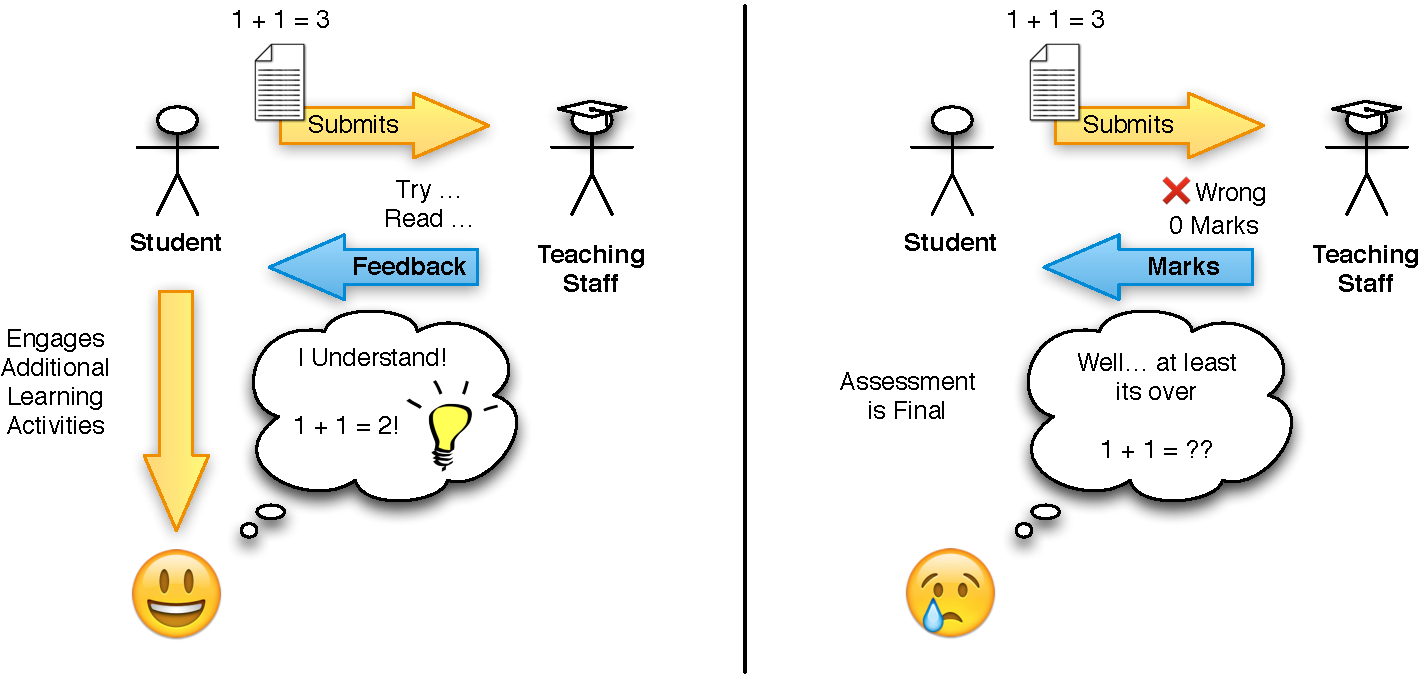
\includegraphics[width=\textwidth]{FormativeLearning}
	\caption{Formative feedback enables an ongoing learning process, with feedback providing details on how work can be completed rather than being an end in itself.}
	\label{fig:formative_learning}
\end{figure}



\fref{fig:pace} highlights another issue with the use of summative assessment during the teaching period. This figure shows three hypothetical students, Student ``A'', Student ``B'' and Student ``C'', and their depth of understanding over the teaching period. At the start of the teaching period each student comes in with existing knowledge, and during the teaching period they construct additional knowledge. When Assessment 1 (A1) is performed each has achieved some level of understanding that is compared against an expected level of achievement. When summative grading is used at this point Student ``C'' has not made sufficient progress and would receive a low grade: they have learnt too little. At the same time Student ``A'' has not been challenged by this assessment, and there is little recognition for this students advanced understanding: they have learnt too much. Student ``B'' is somewhere between these two, and therefore receives a ``good'' grade: they have learnt just enough. The first assessment is punishing Student ``C'' for learning these topics too slowly, and is discouraging Student ``A'' by not recognising their current level of understanding. There is also little distinction between Student ``A'' and Student ``B'', from this perspective they are the same.

\begin{figure}[h]
	\centering
	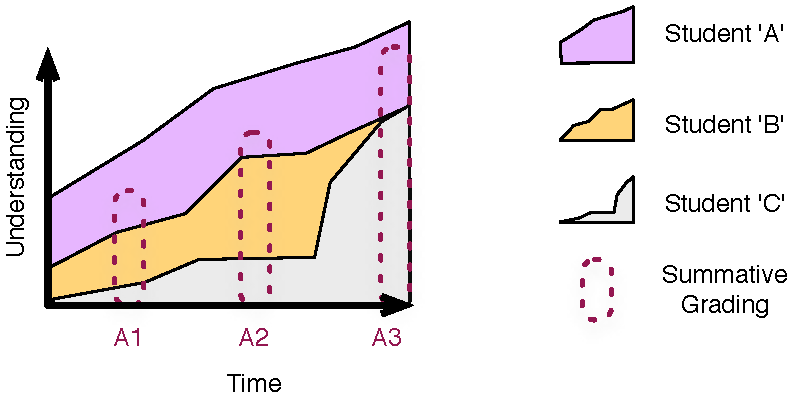
\includegraphics[width=0.8\textwidth]{PaceOfLearning}
	\caption{A hypothetical scenario, showing summative grading measuring pace of learning.}
	\label{fig:pace}
\end{figure}

Similar patterns occur for the second assessment (A2) later in the teaching period. Student ``A'' is still not begin challenged, Student ``B'' is progressing nicely, and Student ``C'' is struggling. For Student ``C'' this negative reinforcement may possibly discourage them from attempting to master the concepts, and reinforce any negative opinion they have of the field in general. In this case, however, Student ``C'' more fully grasps the concepts after the completion of the second assessment. The concepts start to come together, and by the end of the unit Student ``B'' and Student ``C'' have a comparable depth of understanding. This result will, however, not be reflected in their results. Given that each of the assessment items in our hypothetical unit were summative, Student ``C'' will have lost significant marks from the first two assessment items. In effect, the summative assessment is not only assessing the final level of understanding, but also the pace at which the student was able to achieve this understanding. 

This grading during the semester is also not effective for helping the high achieving Student ``A''. At no point has their advanced knowledge been recognised, and the constrained nature of the assessments are not likely to have helped their development. 

\fref{fig:formative} shows an alternative picture, one that makes use of formative feedback and delays all summative assessment to the end of the teaching period. At each of the assessment points during the semester the students each receive formative feedback based on their individual level of understanding demonstrate at that point. The advanced standing of Student ``A'' can be recognised, and the student can be encouraged to further their understanding with additional resources and advice. Student ``B'' can be congratulated for making good progress, their misunderstandings can be addressed and they can be advised how best to proceed with the upcoming material. Student ``C'' can be offered additional support or directed to useful resources, their lack of progress is not punished but used to indicate the student needs additional help. This more personal help and attention should result in improved learning, but even when the progress remains the same the summative assessment at the end of the semester is still a better representation of the students' learning outcomes.

\begin{figure}[h]
	\centering
	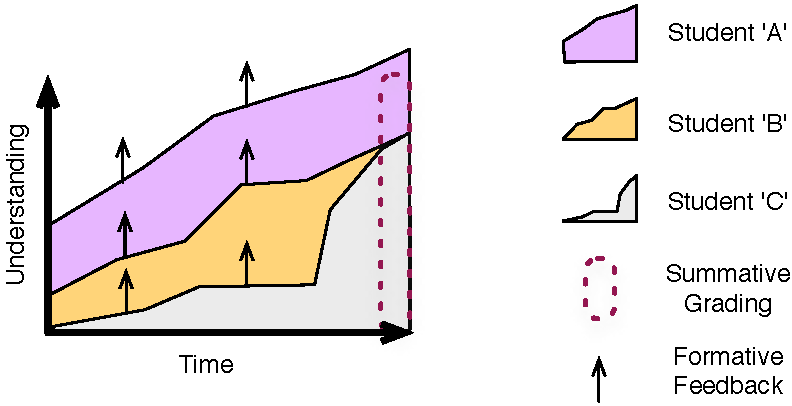
\includegraphics[width=0.8\textwidth]{FormativeFeedback}
	\caption{An alternative to \fref{fig:pace}, showing formative feedback supporting learning during delivery with summative grading at the end.}
	\label{fig:formative}
\end{figure}

To best support student construction of knowledge the model presented in the next chapter aims to maximise the use of formative assessment: assessment that supports learning. This involves the use of frequent formative feedback during the semester to aid students in developing appropriate understanding, and delaying summative assessment until after unit delivery.

Our assessment should, as much as possible, focus on providing feedback on student understanding and ability to meet the intended learning outcomes. We want to focus on more than just the ``product'' outcomes from the teaching and learning activities. Assessment tasks need to include aspects that require students to articulate their current understanding of concepts. This can then be used to help determine the students current level of understanding, and errors evident in this work provides opportunities for students to learn from their mistakes. 

This principle relates to both students construction of knowledge and to the alignment of activities and assessment, as shown in \fref{fig:how_principles}. Formative assessment of learning outcomes during delivery helps students in the construction of knowledge, providing opportunities to learn from their mistakes without fear of losing marks. These formative tasks also help both staff and students with the alignment of teaching and learning activities and assessment tasks. Staff can use the identified misunderstandings to help guide students individually, and to change or adjust teaching and learning activities where needed. For students, this ongoing focus on articulation of understanding and receiving feedback will ensure they are suitably prepared to demonstrate how they have met all of the intended learning outcomes in the final summative assessment.

The summative assessment also contributes to both students construction of knowledge and to the alignment of activities and assessment. For final unit grades students will need to demonstrate how their understanding aligns with the units intended learning outcomes. The assessment needs then to aim to assess the learning outcomes, evaluating how suitable the students level of understanding is at the end of the unit. The SOLO taxonomy (Structure of the Observed Learning Outcome) proposed by \citet{Biggs:1982} provides effective guidelines for performing such an assessment.

To summarise, the model presented in \cref{cha:approach} aims to enhance learning outcomes through the use of frequent formative feedback. This will meet the requirements taken from \citet{Gibbs:2004}, thereby avoiding the issues raised by \citet{Smith:2005}. To be effective, formative feedback must be communicated effectively to students and provide them with clear means of addressing any shortcomings.

% subsection aim_to_assess_learning_outcomes_not_learning_pace_or_product_outcomes_ (end)

\subsection{Focus on important aspects, while providing access to necessary details.} % (fold)
\label{ssub:focus_on_important_aspects}

Adopting constructivist learning theories requires a recognition that ideas cannot be directly communicated, and that teaching is therefore not about presenting the required material but guiding students to actively construct their own understanding of the required topics. To accommodate this change in approach, teaching staff need to carefully plan communication so that it focuses students appropriately on the most important aspects. In communicating concepts it is important to focus on only core aspects, ignoring unnecessary details. To borrow an idea from communication theory, we aim to have as high a signal to noise ratio \cite{Shannon:1949} as possible, ensuring students will not miss important details amongst the noise, no matter how interesting teaching staff find particular side issues.

Presentation of teaching and learning resources need to take into consideration their purpose when determining what is communicated. For example, lectures are not a suitable means of communicating details, but could be useful for inspiring students, and motivating them to learn a particular topic. In these situations, the focus should therefore be on providing only key aspects necessary for students to get started with a topic, or important concepts to guide their thinking. Further resources can then provide students with access to relevant details as they are required, and when they will be appropriate for each student.

With limited resources, primarily time, a classic depth-vs-breadth trade off also needs to be considered, when thinking about the focus on a particular unit. Given that we have fixed time, it is important to aim to cover an appropriate breadth and depth of topics, as illustrated in \fref{fig:depth}. Different units could aim either for a wide breadth and shallower depth, or for a narrower focus with a deeper depth.

\begin{figure}[htbp]
	\centering
	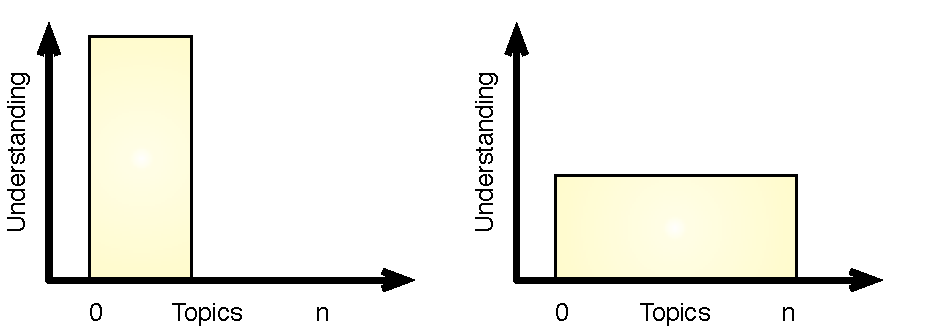
\includegraphics[width=0.75\textwidth]{DepthOrBreadth}
	\caption{Given a fixed teaching ``volume'', a unit can cover either a breadth of topics or fewer topics in depth.}
	\label{fig:depth}
\end{figure}

%
% JG - are there other studies supporting this that can be cited??
%

The SOLO Taxonomy \cite{Biggs:1982} provides several levels that can then be used in defining appropriate intended learning outcomes, as described in \citet{Biggs:1996c} and further elaborated upon in \citet{Biggs:2007}. These have been found to be effective means of communicating intended learning outcomes across a range of fields and units \cite{Brabrand:2007,Brabrand:2009}. Biggs recommends that university level degrees should aim for relational levels of understanding, indicating that in many regards a focus on depth is more appropriate than a shallow understanding across a wider range of topics.

Interestingly, the study conducted by \citet{Schwartz:2009} found that high school students who reported studying a major topic in depth earned higher grades in college than those who reported covering no topics in depth. If this translates to undergraduate computing education, then a depth of understanding in programming may help students succeed with other computing units. The strong correlation generally observed between programming skills and other computing skills \cite{McGettrick:2005} supports this idea.

As programming is central to the discipline of computing \cite{McGettrick:2005} it will be important to focus on building depth of understanding, over covering a breadth of topics. This is particularly challenging as external parties seek to inject more content into curriculum. There is a constant pressure to include details on contemporary topics such as developing for mobile devices, web application programming, building graphical user interfaces, using certain programming languages, development environments, or software tools. Introducing such topics may have some merit, but introduces the risk of inappropriately focusing students attention. A successful introductory unit should focus on building sufficient depth of understanding such that additional topics can be learnt by the student on their own. In contrast, where a breadth approach is taken students may learn contemporary tools at the risk of missing the underlying concepts that would enable them to move beyond what they have learnt.

By focusing on important aspects the teaching and learning activities and assessment tasks will help guide students in the construction of their knowledge, and ensure that they align to sufficiently deep cognitive levels. As tasks define what students will do, this in turn helps to ensure that students are developing appropriately deep knowledge in relation to the intended learning outcomes.

% subsection focus_on_depth_of_understanding_over_breadth_of_coverage_ (end)

\subsection{Communicate high expectations} % (fold)
\label{ssub:have_high_expectations_of_students_}

Communicating high expectations was an important part in the development of the model. In listing their principles for good undergraduate education, \citet{Chickering:1987} include \emph{communicating high expectations} as one of their seven principles. \citet{Chickering:1987} state ``expect more and you will get more'' and indicate that high expectations are important for everyone -- from those who are poorly prepared or unwilling, to exert themselves to those who are bright and motivated. Similarly, \citet{Klem:2004} reported that elementary and secondary school students were likely to be more engaged with learning if they perceived their teachers as using a well structured environment with high expectations. 

Believing in students' potential is also key to the approach presented by \citet{Soetanto:2003,Soetanto:2012}. Soetanto's approach aimed to improve students' discipline, confidence and belief in their potential, and units delivered with this approach have gained in popularity despite their technical difficulty and being delivery in a foreign language (English). 

By having high expectations of our students we aim to build student confidence and to get them to aspire to excellence. High expectations require students to work hard throughout the unit's delivery, providing encouragement to spend sufficient time on the teaching and learning activities. This then requires both time and energy from students, which should improve outcomes: as stated by \citet{Chickering:1987} ``time plus energy equals learning''.

% subsection have_high_expectations_of_students_ (end)

\subsection{Actively support diverse student efforts} % (fold)
\label{ssub:actively_support_student_efforts}

Both \citet{Chickering:1987} and \citet{Soetanto:2003,Soetanto:2012} indicate high expectations should also apply to teaching staff. If the students are to meet our high expectations, they will need our active support. This will need to extend beyond providing formative feedback, to providing active support throughout the process. Given the technical nature of introductory programming and the exacting nature of a compiler, students typically face numerous challenges.

This requires the recognition of student differences, and preferred learning styles. The various works on learning styles \cite{Coffield:2004} indicate that individuals have different preferences with how they approach their learning. By providing support for a range of learning approaches, and through using different ways of communicating the same ideas, the model aims to help students in the construction of their knowledge. Providing a range of resources will enable students to approach concepts and topic from a variety of angles.

% subsection actively_support_student_efforts (end)

\subsection{Trust and empower students to control their own learning} % (fold)
\label{ssub:trust_and_empower_students_to_control_their_own_learning}

%
% JG - I think this is very nice discussion :-)
%


Student motivation has a significant impact on learning. In terms of strategies for improving student motivation, McGregor's work on motivational strategies in business \cite{McGregor:1960} provides some insight into similar strategies that could be applied to education, these ideas are summarised in \tref{tbl:theoryx_y}.  In regards to personnel management, McGregor identified two categories of managers perceptions of their employees: named ``Theory X'' and ``Theory Y''. 

\begin{itemize}[noitemsep,nolistsep]
	\item Traditional businesses were seen to use coercion or persuasion as a strategy to motivate employees to achieve required levels of productivity. These strategies are used when managers adopt the view that employees do not want to work and cannot be trusted, \citet{McGregor:1960} named this understanding of human motivation as Theory X. 
	\item In contrast, Theory Y assumes that, given the right conditions, people want to work, that they can be trusted and will do their best work when they are.
\end{itemize}


While originally applied to business organisation management, these views can also be applied to an educational setting. \citet{Markwell:2004} categorised Theory X and Theory Y positions for educational settings, as summarised in \tref{tbl:theoryx_y}. In the educational context Theory X can be categorised as:

\begin{itemize}[noitemsep,nolistsep]
	\item Being dominated by a negative view of students and their motivation. 
	\item Seeing staff as central to the distribution of knowledge.
	\item Believing that students must be coerced into learning. 
\end{itemize}

The role of the teacher is seen more as a \emph{sage on a stage}.These attitudes are unlikely to lead to student-centred approaches to learning, and conflict with constructivist thinking.

The contrasting Theory Y position takes a more positive view of students, their potential and willingness to learn. Students are viewed as being naturally inquisitive, willing to learning, and capable of engaging appropriately with the learning activities. The role of the teacher is seen more as a \emph{guide by the side}. The resulting teaching and learning context is likely to lead to student-centred approaches that are more in keeping with constructivist thinking.

These two perspectives represents the two extremes, and no one individual is likely to hold a pure Theory X or Theory Y position. \citet{Markwell:2004} differentiated between a Hard and Soft form of Theory X. Hard Theory X teachers focus on the punitive aspects of the assessment, focusing on the punishments for not following the rules. While Soft Theory X uses marks for encouragement, with the use of bonus marks or similar motivations. In contrast, Theory Y focuses on providing opportunities and resources for students to learn from.

In order to achieve many of the principles listed here it is necessary to adopt a predominantly Theory Y stance. The formative nature of the assessment tasks together with the high expectations will both require a level of trust in students that cannot be achieved with a predominantly Theory X stance. High expectations of students is a natural repercussion of a Theory Y position, and enhancing motivation in this way will ideally help students in the construction of their knowledge.

\begin{landscape}
 \renewcommand{\arraystretch}{1.6}
 \begin{table}[htbp]
 	\caption{Comparison of ``Theory X'' and ``Theory Y'' attitudes in education, adapted from \citet{Markwell:2004}}
 	\label{tbl:theoryx_y}

    \begin{tabular}{p{4in}|p{4in}}
    \textbf{Theory X} & \textbf{Theory Y} \\
    \hline
    Students have little desire to learn new material. & Students want to learn, learning is as natural to students as play or rest. \\
    Students are inherently lazy and will attempt to get the material dumbed-down; the teacher must use a controlling environment to force students to learn and prevent cheating. & Students are not lazy; threats of diminished grades are not necessary to motivate students. The self-satisfaction from learning is sufficient to commit students to achieving the educational objectives. \\
    Students prefer to be directed and do not want to be responsible for their own learning. &  Students will naturally accept responsibility for learning. \\
    The teacher must act as the source of information and actively transmit it to the students. &  The intellectual potential of most students are being only partially utilized in the classroom. \\
    Many students are not capable of learning the necessary material and can be expected to earn a low grade. & Imagination, ingenuity, and creativity are widely distributed within the student population and will be willingly applied to the learning process. \\
    \end{tabular}
 \end{table}
\end{landscape}

% subsection trust_and_empower_students_to_control_their_own_learning (end)

\subsection{Embed reflective practice in all aspects} % (fold)
\label{ssub:embed_reflective_practice_in_all_aspects}

In education the idea of reflective practice is to periodically look back at our teaching, and consider how things can be improved. The foundations of this idea can be traced back to \citet{Dewey:1933}, though reflective practice itself was originally proposed by \citet{Schon:1983}. \citet{Farrell:2007,Farrell:2008} identified two forms of reflective teaching practice: a strong form and a weak form. In its weak form, reflective practice involves informal evaluation of various aspects of professional practice that \citet{Farrell:2008} likens to a ``thoughtful practice''. The alternative strong form of reflective practice involves systematic reflection on teaching and taking responsibility for teaching and learning activities. For reflection to be effective, \citet{Richards:1994} state it must be used ``hand-in-hand'' with critical self-examination with reflection being the basis for decision making, planning and action.

Reflection plays an important role for both staff and students in the model presented in \cref{cha:approach}. Students undertaking units taught using this model will graduate and move into professional practice. Engaging them with reflective practice throughout their education will help ensure they are adequately equipped for lifelong learning \cite{Field:2006}. The active incorporation of frequent formative feedback provides a direct means of encouraging students to reflect on their work throughout the delivery of the unit, and the summative assessment should include some reflective aspects where students can reflect on what they have achieved in the unit.

\begin{figure}[ptbh]
	\centering
	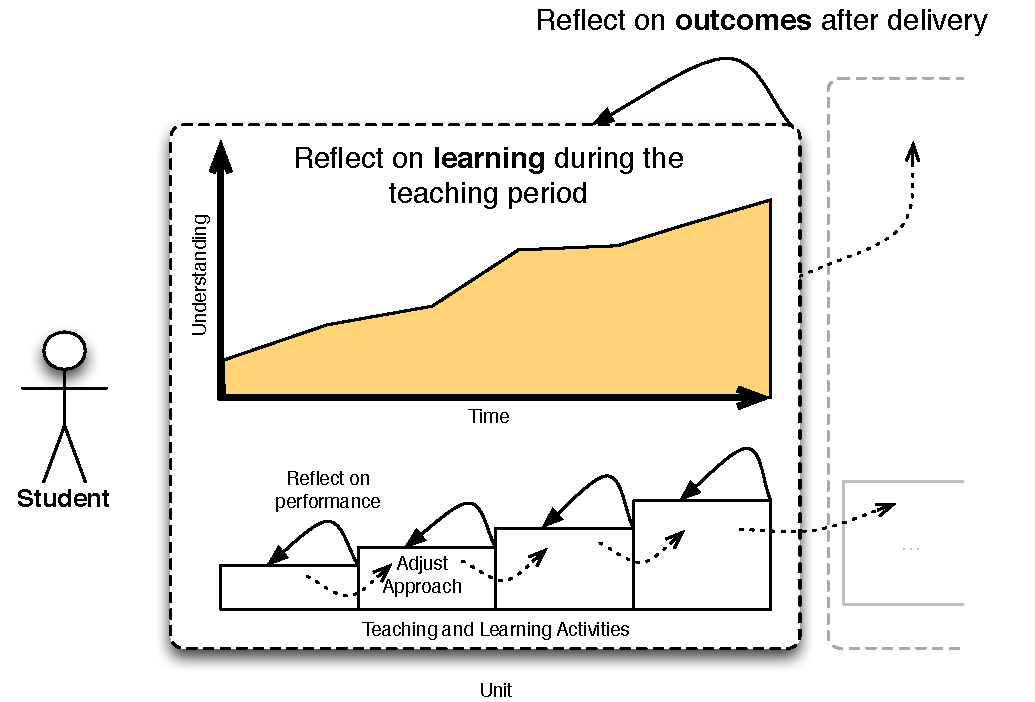
\includegraphics[width=\textwidth]{StudentReflection}
	\caption{Students reflect on their learning during the teaching period, and on the outcomes they have achieved after the teaching period.}
	\label{fig:student_reflection}
\end{figure}

The role of reflection, with respect to the teaching and learning activities, for students is shown in \fref{fig:student_reflection}. When each learning activity is concluded, students are encouraged to reflect on their learning. In this process students identify any areas they would like feedback on, and can use this to ensure their formative feedback is relevant to their current situation. By reflecting, and through the subsequent formative feedback, students reinforce the construction of their knowledge, and are able to inform their actions for upcoming teaching and learning activities.

At the end of the teaching period for a unit, students are encouraged to reflect on their unit as a whole. Students can reflect on their achievements, challenges overcome, work habits and other aspects they felt influenced their learning. This process of reflection should help students consolidate their knowledge, drawing into clear focus exactly what they have achieved and, hopefully, ways they can improve their learning in future semesters.

\fref{fig:staff_reflection} shows the role of reflection for teaching staff. During the teaching period staff reflect upon the delivery of the teaching and learning activities and student progress. Common misconceptions of students identified in formative feedback can be used to update delivery during the teaching periods. After the teaching period students' results -- both in terms of grade distributions and quality of evidence demonstrated in the final summative assessment -- can be drawn upon to suggest changes for subsequent unit deliveries. Reflections on teaching should be shared amongst all teaching staff related to the unit to encourage reflective practice, and to facilitate collaborative improvements.

\begin{figure}[ptbh]
	\centering
	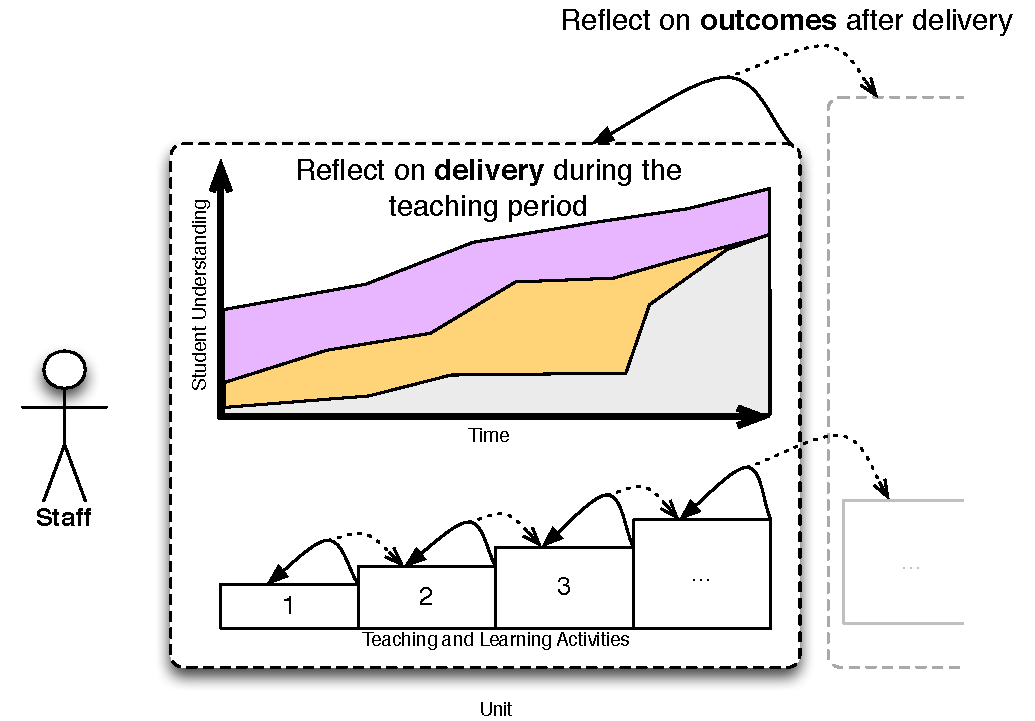
\includegraphics[width=\textwidth]{StaffReflection}
	\caption{Staff relect on delivery during the teaching period, and on the outcomes students achieved after the teaching period.}
	\label{fig:staff_reflection}
\end{figure} 

Reflection underpins all of the principles presented. Students engage in reflection as a tool to help them construct their knowledge, and the formative feedback activities enable student and staff reflections. Staff reflect on teaching and learning activities, their alignment to learning outcomes, and the depth and breadth of coverage. Reflections enable educators to realistically manage expectations of students, the support offered, and to help balance trust with mechanisms to avoid inappropriate behaviour. Even the very nature and composition of these principles have been the focus of ongoing reflective practice.

To ensure ongoing improvements for both students and staff, the model incorporates reflective practice across all aspects. Students engage in reflection throughout the learning process, using their reflections to direct formative feedback and consolidate knowledge. Teaching staff reflect on delivery, progress, and outcomes to improve the teaching and learning environment to better meet student needs.

% subsection embed_reflective_practice_in_all_aspects (end)


\subsection{Be agile and willing to change} % (fold)
\label{ssub:be_agile_and_willing_to_change}

For reflective practice to actively enhance teaching educators must embrace change, focusing on aspects that will deliver the most value for students for the effort required. Similarly, as software developers this emphasis on delivering value by ``\emph{focusing on the things that matter most}'' is reminiscent of the agile software development principles \cite{Martin:2003}. The agile software development community aimed to move away from heavyweight, documentation driven, software development processes toward a more \emph{agile} approach focused on outcomes. \citet{Beck:2001} documented the Agile Manifesto; the key priorities from a wide range of agile software development processes. The Agile Manifesto states the value of: 

\begin{itemize}[noitemsep,nolistsep]
	\item \textbf{individuals and interactions} \emph{over} processes and tools,
	\item \textbf{working software} \emph{over} comprehensive documentation,
	\item \textbf{customer collaboration} \emph{over} contract negotiation, and
	\item \textbf{responding to change} \emph{over} following a plan.
\end{itemize}

In many ways the evolution of software development process from the traditionally heavyweight processes to lightweight agile processes can be likened to a shift from a predominant Theory X environment to one which is predominantly Theory Y. The focus on documentation and rigid control over the development process is being relaxed, and developers are being trusted and expected to deliver value. 

If we are to affect change in education from a mark-driven Theory X environment, to a student-centred Theory Y environment, then the agile software development principles provide useful guidance to inform our model. To realise all of the principles presented in this chapter it is necessary to adopt similar priorities in our teaching, valuing things that help students construct their knowledge over other less valuable activities.

To help manage change effectively we view the education environment as consisting of an a) overall strategy, b) teaching and learning resources, and c) teaching and learning activities, as shown in \fref{fig:strategy}. 

\begin{figure}[htbp]
	\centering
	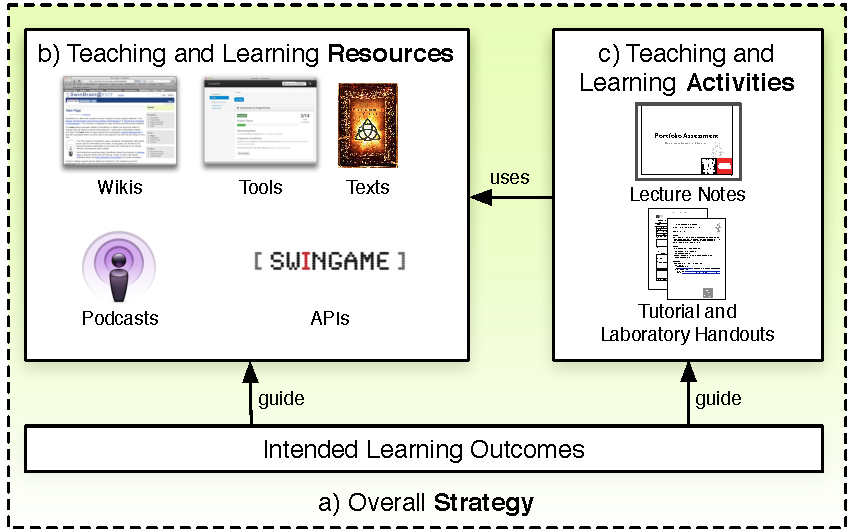
\includegraphics[width=0.85\textwidth]{StrategyResourcesActivities}
	\caption{Relationship between a) overall strategy, b) resources and c) activities used to manage change effectively.}
	\label{fig:strategy}
\end{figure}

The strategy for delivering unit content informs the choice of assessment approach, approach to selecting unit content, and the development of the intended learning outcomes. The central role of the intended learning outcomes means that the overall strategy should not change unless significant issues are identified in the approach overall. Teaching and learning \emph{resources} can then be separated from the teaching and learning \emph{activities}. In this way we can create reusable resources that are independent of the activities that are used in, meaning that activities can be adjusted more freely to better help direct student efforts. An overview of this approach is summarised in the following list, and each of these points are expanded upon in \cref{cha:approach} and \cref{cha:example_impl}.

%
% JG - I am not sure this is "details"...
%
% Do you flesh this out in a later chapter - if so could indicate this -or even forward ref
% and put there???
%
% It raises a lot of "how" questions which might be better deferred to with the answers later?
%


\begin{itemize}[noitemsep,nolistsep]
	\item Develop an \emph{overall strategy} for delivering the unit content. Then:
	\begin{itemize}[noitemsep,nolistsep]
		\item Determine appropriate content, by focusing on important aspects and using principles related to \emph{what} we aim to teach.
		\item Derive intended learning outcomes, using appropriate verbs for the intended levels of the SOLO taxonomy.
		\item Focus teaching and learning resources and activities on engaging students actively with the concepts related to the intended learning outcomes.
		\item Avoid changing overall strategy, unless there are significant issues.
		\item Select an appropriate assessment approach.
	\end{itemize}

	\item Create teaching and learning \emph{resources}.
	\begin{itemize}[noitemsep,nolistsep]
		\item Deliver material following the direction from the overall strategy.
		\item Make resources generic and self contained.
		\item See resources as supporting teaching and learning activities with additional details.
		\item Invest in initial development for long term value; actively reuse and enhance over time.
		% \item Improve integration with delivery material as resources prove to be effective.
	\end{itemize}

	\item Design teaching and learning \emph{activities}.
	\begin{itemize}[noitemsep,nolistsep]
		\item Use these to focus student activity.
		\item Actively review each semester, and rework based on reflection.
	\end{itemize}
\end{itemize} 

% subsection be_agile_and_willing_to_change (end)


% \subsection{Related work on general education principles} % (fold)
% \label{ssub:related_work_on_education_principles}

% %
% % JG - I am not sure about this section in terms of fit & content...
% %
% % Maybe could incorporate in the principles sections???
% %
% %


% In discussing how to improve undergraduate education, \citet{Chickering:1987} listed seven principles for good practice in undergraduate education. These are practices that:
% \begin{enumerate}[noitemsep,nolistsep]
% 	\item Encourages contact between students and faculty.
% 	\item Develops reciprocity and cooperation among students
% 	\item Encourages active learning
% 	\item Gives prompt feedback
% 	\item Emphasizes time on task
% 	\item Communicates high expectations
% 	\item Respects diverse talents and ways of learning
% \end{enumerate}

% The following list states how each of the principles from \citet{Chickering:1987} are integrated with the principles underlying this work. 
% \begin{itemize}[noitemsep,nolistsep]
% 	\item The strong emphasis on frequent formative feedback should be used to help encourage contact between students and faculty. (\Pref{itm:formative}, \Pref{itm:support})
% 	\item This same formative process should also be harnessed to encourage sharing and cooperation amongst students. (\Pref{itm:formative},\Pref{itm:support},\Pref{itm:theory_y})
% 	\item The central nature of the students in constructing their knowledge necessitates an approach that encourages active learning. (\Pref{itm:construct},\Pref{itm:theory_y})
% 	\item The formative feedback process needs to ensure that work is returned promptly to students, ensuring they receive the feedback while it is still relevant. (\Pref{itm:formative})
% 	\item Communicating high expectations is included directly in our principles. (\Pref{itm:expectations})
% 	\item Assessment and teaching and learning activities need to be flexible, enabling different styles of learning and to engage with students diverse talents. (\Pref{itm:support})
% \end{itemize}

% For outcomes based education, 

% \citet{Killen:2000} lists the 

% subsection related_work_on_education_principles (end)


\subsection{Summary} % (fold)
\label{ssub:summary_of_principles_on_how_to_teach}

This section presented nine principles to guide decisions that together should produce a student-centred, constructively aligned, learning environment. Each principle is backed by a range of education theories, and, if valid, together the principles should enable the creation of an environment that is demanding but supportive, focused on students building knowledge, agile, constantly improving through reflections, and accepting of various individual strategies and pace of learning.

% The next section details the principles related to \emph{what} we are going to teach.

% subsection summary_of_principles_on_how_to_teach (end)


% section principles_for_how_the_environment_should_operate (end)






\clearpage
\section{Principles to guide what we should teach} % (fold)
\label{sec:principles_to_guide_what_we_should_cover}

Principles specific to teaching introductory programming are presented in the following list. While the general principles helped shape the overall teaching and learning environment, these principles helped shape specifics in the curriculum, activities, and assessment tasks.
\begin{itemize}[noitemsep,nolistsep]
	\item Set the strategy, and structure learning, around a programming paradigm. (\Pref{itm:paradigm})
	\item Focus on programming concepts \emph{over} language syntax. (\Pref{itm:concepts})
	\item Use programming languages as they were designed to be used. (\Pref{itm:authentic})
	% \item Program code is not, by itself, a suitable means of measuring learning outcomes.
\end{itemize}


%
% JG - I suggest summarise the items from the subsections briefly here
%


Each of these principles is expanded upon in the following sections, and linked to associated research.


\subsection{Set the strategy and structure learning around programming a paradigm} % (fold)
\label{ssub:strategy_around_paradigm}

The programming paradigm chosen for introductory programming can have a large impact on the way the unit is taught and, therefore, the unit's intended learning outcomes. To endeavour that the foundations of a unit do not need to change, a programming paradigm, such as the procedural, functional or object oriented paradigm, needs to be chosen.This will then form the core of the overall strategy for the unit.

Which programming paradigm should be taught first is a popular topic in computing education research. The following list indicates the range of approaches from imperative-first to objects-first approaches.
\begin{itemize}[noitemsep,nolistsep]
	\item Imperative programming first such as with \citet{Koffman:1988a}.
	\item \citet{Cooper:2003} suggest a course working with graphics prior to introductory programming to help students with problem solving skills.
	\item \citet{Felleisen:2004} described a approaching to teaching introductory programming using the functional paradigm and the Scheme programming language.
	\item \citet{Howe:2004} presented a components-first approach.
	\item \citet{Bennedsen:2004} argued for the use of a model-first approach using the object oriented programming paradigm.
\end{itemize}

 With the predominant role of objects in industry, a common trend has been to move from imperative-first approaches to objects-first approaches. This approach has ``failed'' according to \citet{Astrachan:2005} and \citet{Reges:2006}. While \citet{Ehlert:2009} reported no significant difference between approaches using objects-first and objects-later, their later work \cite{Ehlert:2010} indicated the objects-later approach had a greater comfort level for students. \citet{Robins:2003} include the imperative-first and objects-first approaches as one of their four themes from the literature on learning and teaching introductory programming. \citet{Lister:2006a} provide an in depth look at the research perspectives on the topic of objects-first, but in general there is no consensus on which approach should be taken.

The design of the introductory programming units developed in this research work there was a need to choose which \emph{x}-first approach will be used. The main decision seemed to be between the imperative-first, objects-first or functional-first approaches. Whichever approach is taken, the choices guide which concepts are covered in the unit and the order in which these can be tackled.

% subsection set_the_strategy_and_structure_learning_around_programming_a_paradigm (end)

\subsection{Focus on programming concepts} % (fold)
\label{sub:focus_on_programming_concepts}

There are various views of programming in the literature. On perspective views programming from a mathematical basis \cite{Denning:1989,Dijkstra:1989,Hoare:1969}, others see it as an exercise in problem solving \cite{Palumbo:1990}, modelling concepts \cite{Bennedsen:2004}, though most textbooks approach the topic through language syntax and features \cite{Robins:2003}. In this work we avoided the standard textbook approach, and instead we focused on programming concepts.

A similar idea was expressed in \citet{Goldman:2004} as a \emph{concept based} approach. The work introduced students to a number of ``big ideas'' related to software development using the JPie interactive programming environment. Our approach differs in that we focus on the ``small ideas'' that programs are build upon. In this way we build depth across these ideas rather than breadth, in line with our general principles.

Topics such as variables, procedures, control flow, etcetera are each approached as a concept. This is similar to the model-based approach of \citet{Bennedsen:2004}, but applied to procedural programming concepts. By focusing on concepts we aim to provide students with reasons why the various programming features should be used, when different abstractions should be used, and help students develop means of understanding these abstract ideas. This concept based approach can be applied to procedural programming concepts, object oriented programming concepts, and other programming paradigms.

Winslow's comparison study of expert and novice programmers \cite{Winslow:1996} indicated that expert programmers tend to ``abstract from a particular language to the general concept''. By focusing on the concepts first we hope to instil similar expert-like ideas in the students. Students are encouraged to create \emph{conceptual programs}, which can then be mapped to code using the programming language syntax rules. Focusing first on the concepts should encourage a depth of understanding, with students going beyond surface learning of the syntax used and thinking conceptually about what they are trying to achieve.

Programming concepts are tightly interrelated, and yet there is a need to provide a sequence of activities that can be introduced to students without overloading them initially. In designing these activities we aimed to ensure that concepts could be introduced to students in such a way as to reduce the amount of ``magic'' to a minimum. Limiting the cases where students had to do something without being able to reason why with the concepts covered so far.

The aim of this is to enable students to explore language features. At each stage in the process students should have sufficient concepts to be able to understand the programs they are asked to create. To extend students further they can be asked to experiment with features, using the concepts covered to create programs they are interested in. Ideally this would enhance student motivation, and ensure they spend sufficient time on the task.

The focus on programming concepts means there is a need to: %also in supporting chapter
\begin{itemize}[noitemsep,nolistsep]
	\item Introduce programming concepts incrementally;
	\item Provide students with time to put concepts into practice;
	\item See syntax as a means to an end, not an end in itself;
	\item Avoid using language features before concepts that can explain their use; and
	\item Map concepts to code using programming language grammars.
\end{itemize} 

% section principles_to_guide_what_we_should_cover (end)

\subsection{Use programming languages as they were designed to be used} % (fold)
\label{ssub:use_programming_languages_as_they_were_designed_to_be_used}

While we agree with the ``back to basics'' approach of \citet{Reges:2006}, we want to emphasise using programming languages in the way they were designed to be used. Our emphasis on programming concepts has deliberately relegated language to a secondary role, and one that can be changed by learning new syntax rules. Given this, changing between languages is less problematic, and therefore we should not use a language for its industry relevance. Rather, language choice should be based on the programming concepts it supports, its available across computing platforms, and the level of support it offers novices.

Programming language choice for introductory programming is as popular in the Computing Education Research literature as the choice of programming paradigm. The following list covers a select number of well-cited papers on which programming language to use in teaching introductory programming, ordered by year it shows the shift from procedural languages to object oriented languages.

%
% JG - I suggest rethink the use of this long list approach
%



\begin{itemize}[noitemsep,nolistsep]
	\item \citet{Koffman:1988} argued for Modula-2 over Pascal, PL/1 and Ada, 
	\item \citet{Mody:1991} argued against C, and C++ for its lack of coherence, simplicity, understandability and implementability. 

	\item \citet{Roberts:1993} discusses Stanford's shift from Pascal to C, addressing common issues with C by providing libraries to encapsulate complex features, emphasising procedural and modular abstractions, and focusing on the discipline of software engineering.

	\item \citet{Brilliant:1996} discussed programming paradigm and language selection for introductory programming. They concluded that there was no clear advantage to starting with either procedural programming, object-oriented programming, or functional programming paradigms. In terms of language they discussed moving from Pascal to Ada, C, C++, or Scheme.

	\item \citet{Boszormenyi:1998} argued for Modula-3 over Java, discussing features that are useful to be taught in introductory programming yet missing from Java.

	\item \citet{Howell:2003} claimed that through structured labs, comprehensive grade sheets, in-class grading and frequent feedback any programming language could be used.

	\item \citet{Gupta:2004} suggested that a first language should strike a balance between being easy to grasp and supporting advanced concepts needed for later units.

	\item \citet{Kelleher:2005} provided a detailed examination of a wide range of programming languages used for teaching introductory programming. Their work discussed various efforts to help make programming more accessible for novices, including systems that range in support from look at the way programs are expressed, how programs are structured, understanding of program execution, to systems that embed learning support. While the work reported on a range of systems it does not provide any recommendations on which language to use.

	\item \citet{Bishop:2006} presented the pros and cons, from their experiences, in using the C\# programming language, and provided some recommendations for those looking at using the language.

	\item \citet{Mannila:2006} argued for the use of Python due to its simplicity, with examples comparing Python to Java.

	\item \citet{Mannila:2006a} provided a set of criteria for comparing language features for introductory programming. The study then compared several languages, with Eiffel, Java and Python achieving the highest scores.

	\item \citet{Pendergast:2006} provided a reflection on teaching introductory programming with Java over a number of years, highlighting some of the issues encountered and mechanisms to avoid these.

	\item \citet{Maloney:2010} described the Scratch programming environment, a visual programming language designed primarily for students aged between 8 and 16.

	\item \citet{Anik:2011} used the Analytic Network Process methodology to help guide the decision of which language should be used first. The relative weightings given to the various aspects resulted in Java being ranked above the other languages.
\end{itemize}

Interestingly, underlying many of these papers is the idea that switching language is difficult. For example, \citet{Brilliant:1996} indicated that teaching multiple languages increases the overhead necessary to cover language details and peculiarities. By having a focus on programming concepts over language syntax this work aimed to tackle this problem from a different angle. In our previous teaching we noticed that students tended to focus on or ``cling'' to syntax. Shifting language was a major effort as it was syntax they had learnt. Students felt they were ``Java programmers'' or ``C/C++ programmers''; they did not see that they were learning something far more important, they were not learning a specific language, they were learning to program. 

This focus also becomes evident when you examine the title of many introductory programming units. Introductory programming unit titles like ``Introduction to Programming with C'' and ``Software Development in Java'' give the impression that the language is important, raising its role from supportive to central in the unit.

%
% JG - again, perhaps "was" -> "is guided by" - I assume OTHERS could chose diff langs but still fulfil the principles??
% 
% 
% 


Choosing a language for the \emph{concept-based} approach to introductory programming was guided by the following principles:
\begin{itemize}[nolistsep,noitemsep]
	\item \textbf{Focus on programming concepts} \emph{over} language syntax.
	%Remember we are not teaching a language, we are teaching students to program.
	\item \textbf{Teach students to learn the language} \emph{over} teaching the language explicitly.
	%Do not teach the language explicitly, teach students to learn languages themselves.
	\item \textbf{Value languages that support the concepts to be learnt} \emph{over} the languages that are the current industry trend.
	%Choose a language, or languages, that support the concepts that need to be covered.
	\item \textbf{Use languages that support multiple operating systems} \emph{over} those tied tightly to a single platform. 
	%Ensure support for multiple operating systems, enabling students to use their preferred platform.
	\item \textbf{See multiple languages as an important part of the learning} \emph{over} focusing on a single language.
	%See multiple languages as an important part of the learning, not an unnecessary overhead.
	\begin{itemize}
		\item Use multiple languages to encourage students to focus on concepts over programming language syntax.
		\item Expose students to language differences enabling them to see different strengths and weaknesses. 
		\item Encourage students to see that they are learning to program, not learning one programming language.
		\item Foster the attitude that language is a choice, students should not feel constrained to one language and should be open to possibilities other languages offer.
	\end{itemize}
\end{itemize}

As with the Agile Manifesto, we agree that there is value in the items on the right, but we value the items on the left more.

One aspect that is different from other work is the importance of the use of the language in industry. If the concept based approach is successful students will be able to quickly develop skills in industry relevant languages in later units. The first units can focus on using languages that best meet educational requirements, while later units can cover language specific details and peculiarities briefly knowing students have an understanding of underlying concepts and the ability to learning new languages themselves. 

% \cite{Koffman:1988,Roberts:1993,Brilliant:1996}
% Arguments against Pascal 
% \begin{enumerate}
% 	\item Missing language features such as open arrays, function pointers, and string manipulation.
% 	\item Not widely used beyond introductory programming.
% 	\item Lack of data abstraction and information hiding.
% \end{enumerate}


% subsection use_programming_languages_as_they_were_designed_to_be_used_ (end)


\subsection{Summary} % (fold)
\label{ssub:summary_of_principles_for_what_to_teach}

This section proposed the use of a \emph{concept-based} approach to teaching introductory programming. This approach focuses on teaching programming concepts directly, with use of the programming language grammars to help students map concepts to code. The aim of this approach is to help students focus on the concepts, while providing them with tools they can use to learn any relevant programming language. The expected outcome of this approach is that programming language choice is much less important than which programming paradigm choice. 

% subsection summary_of_principles_for_what_to_teach (end)

\clearpage
\section{Summary of Guiding Principles} % (fold)
\label{sec:summary_of_guiding_principles}

This chapter outlined twelve principles related to both \emph{how} and \emph{what} we aim to teach in our constructively aligned introductory programming.
\begin{itemize}[noitemsep,nolistsep]
	\item Nine principles describe \emph{how} the teaching and learning environment should operate:
	\begin{enumerate}[noitemsep,nolistsep]
		\item \label{itm:construct} Recognise that students construct knowledge in response to activity.
		\item \label{itm:align} Align activities and assessment to intended learning outcomes.
		\item \label{itm:formative} Assess learning outcomes, not learning pace or product outcomes.
		\item \label{itm:focus} Focus on important aspects, while providing access to necessary details.
		\item \label{itm:expectations} Communicate high expectations.
		\item \label{itm:support} Actively support student efforts.
		\item \label{itm:theory_y} Trust and empower students to manage their own learning.
		\item \label{itm:agile} Be agile and willing to change in response to measurable indicators.
		\item \label{itm:reflect} Embed reflective practice in all aspects.
	\end{enumerate}
	\item Three principles help guide \emph{what} we aim to teach:
	\begin{enumerate}[start=10,noitemsep,nolistsep]
		\item \label{itm:paradigm} Set the strategy and structure learning around a programming paradigm.
		\item \label{itm:concepts} Focus on programming concepts, not language syntax.
		\item \label{itm:authentic} Use programming languages as they were designed to be used.
		% \item Program code is not, by itself, a suitable means of measuring learning outcomes.
	\end{enumerate}
\end{itemize}

\cref{cha:approach} will outline a model for constructively aligned introductory programming units. The model presented was created through the application of these principles, and the model's ability to embody these principles is discussed.

% section summary_of_guiding_principles (end)

% chapter guiding_principles (end)
%!TEX root = Constructive Alignment for Introductory Programming.tex

\chapter{A Model for Constructive Alignment of Introductory Programming} % (fold)
\label{cha:approach}

\graphicspath{{Figures/CAApproach/}}

\cref{cha:guiding_principles} outlined twelve principles, nine for guiding \emph{how} to create a student-centred learning environment, and three for guiding decisions on \emph{what} should be taught in introductory programming. This chapter proposes a model for applying constructive alignment for teaching introductory programming that is in agreement with the twelve principles.

\sref{sec:overall_strategy} describes an application of the principles in defining the overall strategy for teaching introductory programming, outlining the assessment approach used and the approach taken to deliver this material in a student centred manner. This section argues for the user of portfolio assessment, and provides some guidelines for designing and delivering lecture and tutorial classes. Following this, the general model for constructive alignment is presented in \sref{sec:model}, which describes the overall model, the processes within it, and means for addressing plagiarism. The chapter concludes with a brief summary in \sref{sec:ca_summary}.

\section{Overall Strategy} % (fold)
\label{sec:overall_strategy}

One of the overarching principles from \cref{cha:guiding_principles} is the requirement to be agile and willing to change (\pref{itm:agile}). In discussing this principle, \sref{ssub:be_agile_and_willing_to_change} outlined that teaching and learning resources need to be guided by an overall strategy. The overall strategy informs, and is shaped by, the assessment approach, approach to material delivery, and the approach to the selection of unit content. This section describes the application of the principles from \cref{cha:guiding_principles} to the selection of an assessment approach and approach to material delivery. The discussion of approach to selecting content, and specific intended learning outcomes that follow, are presented in \cref{cha:example_impl}.

\subsection{Assessment Approach} % (fold)
\label{sub:assessment_approach}

Assessment plays an important role in defining what students learn. \citet{Rowntree:1977} indicated the central role of assessment procedures in understanding any education system. This is supported by \citet{Ramsden:2003}, who stated that ``from our students' point of view, assessment always defines the actual curriculum'', and further supported by \citet{Biggs:2007} who indicated that ``students learn what they \emph{think} they will be tested on.'' In presenting their conditions for effective assessment, \citet{Gibbs:2004} discussed the dominant influence of assessment in defining what students focus on, indicating that students are able to distinguish between what assessment requires them to pay attention to, and what is likely to result in effective learning. So the selection of an assessment approach will have a significant impact on the overall strategy for both students and staff. 

Consider a traditional introductory programming, taught using a number of assignments and a final examination. This approach, while commonly used, is not in keeping with several of our guiding principles, as outlined in the following list. 

\begin{enumerate}[noitemsep,nolistsep]
	\item This approach to assessment is teacher-centred, and does not easily incorporate aspects from constructive learning theory, as discussed in \cref{cha:background}.  As a result, some adjustments are required in order to address \pref{itm:construct}.
	\item The teacher-centred nature of the assessment also excludes students from the alignment process, \pref{itm:align}, with staff performing the alignment of assessment tasks with intended learning outcomes resulting in additional opportunities for misalignment, as discussed in \cref{cha:background}. 
	\item Similarly, the use of summative assessment during the semester goes against \pref{itm:formative} with its goal of assessing outcomes, and using frequent formative feedback to aid student learning.
	\item The use of assignments marks to motivate students is also contrary to \pref{itm:theory_y}, with marks being used for motivation in either a hard or soft form of Theory X strategy.
	\item Marked assignments also indicate a finality, with marks being lost or gained when the assignment is assessed. These results are typically final, and therefore provide no incentive for student to reflect on their approach to learning, and to ensure they have more fully understood concepts before proceeding. Alternate assessment strategies, with a greater emphasis on formative feedback, could better encapsulate the ideals of reflective practice, and thereby better meet \pref{itm:reflect}.
\end{enumerate}

As a result, the principles from \cref{cha:guiding_principles} requires us to consider other forms of assessment.
  
%
% this is commonly done e.g. in German universities - and sometimes exams
%  are delayed to a later YEAR (let alone end of unit)...
%

One strategy to address this would be to abandon coursework assignments, delaying final summative assessment to an examination worth 100\% of the student's grade. While this would address \pref{itm:formative}, such a heavy weight examination is very much a hard Theory X approach, and fails to recognise the value of coursework assignments, which have been strongly argued for as in \citet{Gibbs:2004} which provided several strong arguments for coursework assignments, including the following:
\begin{itemize}[noitemsep,nolistsep]
	\item Units that include coursework assignments, in addition to an exam, resulted in higher average marks than compared with units that included no coursework assignments \cite{Chansarkar:1987}.
	\item Students prefer coursework assignments over examinations. A position that is also supported by \citet{Kniveton:1996} who stated that students prefer coursework assignments to exams as assignments assessed a better range of their abilities and enabled them to organise their time to a greater extent.
	\item Students attain better results from coursework than examinations. \citet{Gibbs:1997} indicated a strong positive correlation between the proportion of coursework assignments and average marks. Though, \citet{James:2004} indicated that individual students do not consistently perform better, or worse, on any one form of assessment.
	\item Coursework assignments are at least as valid a form of assessment as examinations:
	\begin{itemize}[noitemsep,nolistsep]
	% 
	% Do you have reference to support this statement: 
	% AC: yes :)
		\item Exams are a poor predictor of future performance \cite{Baird:1985,Gibbs:2004}.
		\item Coursework assignments are a better predictor of long term learning than exam results \cite{Conway:1992}. This supports the idea that students adopt surface approaches to preparing for exams \citet{Marton:1976a, Tang:1999}. 
		%
		% Ditto  - reference(s) to support this needed here ->
		%
		\item The quality of learning is deeper in assignment-based units, when compared to exam-based units \cite{Tynjala:1998,Gibbs:2004}.
	\end{itemize}
\end{itemize}

The challenge, therefore, is to define an assessment approach that enables students to construct their knowledge, uses coursework assignments in a formative manner, and enables 100\% of each student's grade to be determined after the end of the teaching period, with a strong alignment to unit intended learning outcomes.

\clearpage
\subsubsection{Portfolio Assessment} % (fold)
\label{sub:portfolio_assessment}

In proposing Constructive Alignment, \citet{Biggs:1996c} advocated strongly for the use of an assessment portfolio, and indicated that the principles of constructive alignment had evolved with the decision to use portfolio assessment. This work was extended in his later work, presented in \cite{Biggs:1997}, which outlined suggestions for implementing portfolio assessment and a generalised model for instruction design. Further advice and details of the generalised model were presented in \citet{Biggs:2007} book on quality learning at university.

Assessment involves three components, all of which are typically under the control of the teacher \cite{Biggs:1997}. These include \emph{setting criteria}, \emph{selecting evidence} and \emph{making a judgement}. With the assessment portfolio the students take control of \emph{at least} the selection of evidence, as illustrated in \fref{fig:select_evidence}. The portfolio is then a collection of work that the student puts forward for assessment against the unit's intended learning outcomes, which helps avoid the teacher-selected \emph{sampling} effect of exams.

\begin{figure}[htbp]
	\centering
	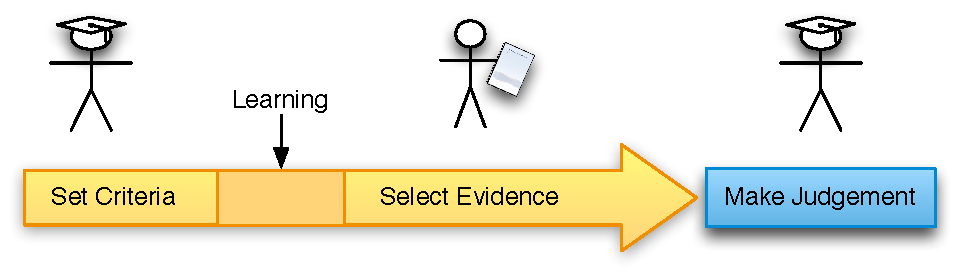
\includegraphics[width=0.8\textwidth]{SelectEvidence}
	\caption{With portfolio assessment the student is responsible for, at least, the selection of evidence in the assessment process.}
	\label{fig:select_evidence}
\end{figure}

%
% Could note that this approach has been used in Architecture and DEsign areas for many years??
% 

\citet{Smith:2001,Smith:2003} identified four different kinds of portfolios evident in the research literature: \emph{dossier}, \emph{reflective}, \emph{training} and \emph{personal development}. These reflect the combination of two identified factors: (a) the purpose of the portfolio as either for selection/promotion or learning, and (b) whether the portfolio is self-directed or mandated. The details of these are described in the following list, and shown in \fref{fig:portfolio_types}.

\begin{description}[noitemsep,nolistsep]
	\item[Dossier] [selection/promotion, mandated] is a portfolio for the purpose of selection or promotion that contains a mandated collection of work to demonstrate achievement. 
	\item[Reflective] portfolios [selection/promotion, self-directed] contain a self selected collection of work that demonstrates growth or accomplishment for the purpose of admission or promotion. The portfolio is accompanied by a self-appraisal, with the justification for the selection of pieces being as important as the evidence itself.
	\item[Training] portfolios [learning, mandated] are a mandated collection of work performed in a learning context. The portfolio has a fixed format, and contains representative work from the student demonstrating acquired skills, knowledge and competencies.
	\item[Personal development] portfolios [learning, self-directed] are a self-selected collection of work, and reflective account of personal growth over an extended period.
\end{description}

\begin{figure}[htbp]
	\centering
	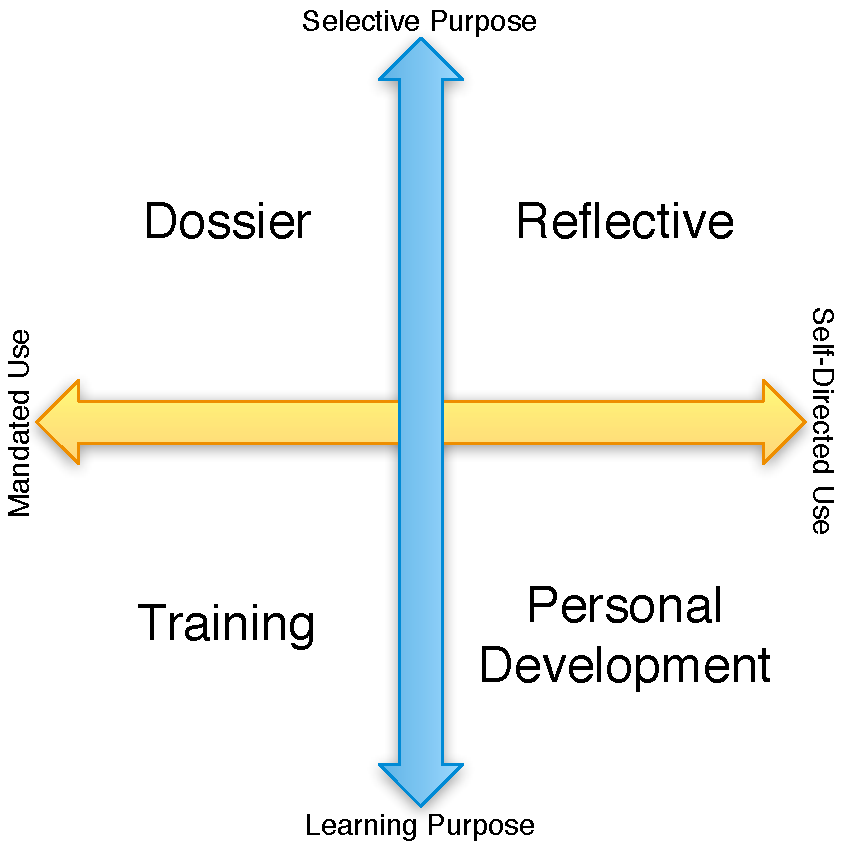
\includegraphics[width=0.50\textwidth]{PortfolioTypes}
	\caption{The four kinds of portfolio based upon purpose and use from \citet{Smith:2001}.}
	\label{fig:portfolio_types}
\end{figure}

Biggs' use of an \emph{assessment portfolio} clearly fits with the \emph{Training} portfolio classification, being a mandated part of the unit assessment for the purpose of evaluating learning outcomes. In the study of a small group of professionals, \citet{Smith:2001} found the training portfolio to be highly rated. Their findings indicated that students found the training portfolio confusing initially, but that once they had understood its function and rational they liked the approach, were easily able to construct their portfolio, and felt it was a fair way to assess their learning.

\citet{Tang:1999} provides further evidence of the value of portfolio assessment. In evaluating how students approach study, they found that students tended to have a narrow, surface approach to studying for tests. These same students were found to adopt wider, more cognitively challenging, approaches when preparing for a portfolio assessment. 

Portfolios have been used to before to assess introductory programming. \cite{Plimmer:2000} reported the successful use of portfolio assessment in an introductory programming unit in which the portfolio contributed between 25\% and 60\% of the students' final grades. Programming portfolios were also discussed by \cite{Jones:2010}, where students submitted a number of portfolio assignments during the semester. These two approaches represent interesting applications of portfolio assessment, but do not use the portfolio as a means of performing a holistic assessment of the students ability to meet the intended learning outcomes, as is proposed in this work.


%
%  Reference if these are quotes?
%  AC: our statement

We argue that when used as a holistic assessment of student performances, portfolio assessment enables a shift from a Theory X ``sage on the stage'' view, to a Theory Y ``guide by the side'' view of education. The traditional approach of setting assignments and exams, in which educators test student ability, becomes inverted with portfolio assessment. Details of the assessment are no longer hidden, as is the case with exams, but is shared with students as the goal they need to achieve. Using portfolio assessment, the emphasis is on the students, and it is their responsibility to demonstrate how they have met a unit's intended learning outcomes. This frees educators to help students and to guide them in the preparation of their evidence. As illustrated in \fref{fig:sage_guide}, we are now working side by side with the students, helping them to achieve the unit's intended learning outcomes. 

\begin{figure}[hb]
	\centering
	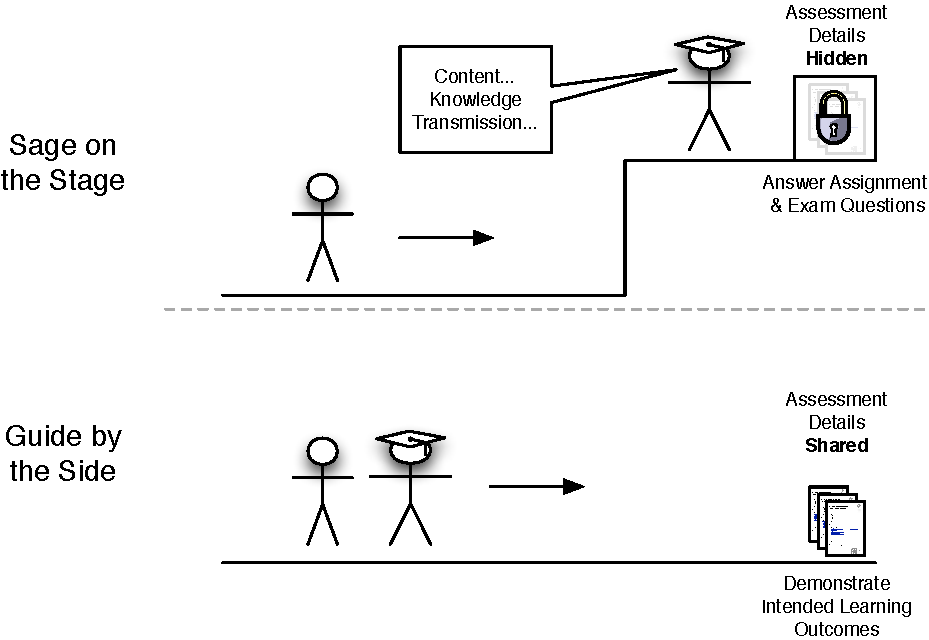
\includegraphics[width=0.90\textwidth]{SageGuide}
	\caption{Portfolio assessment helps enable the view of teaching staff as acting as a ``guide by the side'', rather than a ``sage of the stage''}
	\label{fig:sage_guide}
\end{figure}

%
% This is GOOD!!
%
\clearpage
Portfolio assessment aligns well with all nine ``\emph{how}'' principles listed in \cref{cha:guiding_principles}. 
\begin{itemize}[noitemsep,nolistsep]
	\item The portfolio consists of a collection of work the student feels demonstrates the depth of their knowledge. (\Pref{itm:construct})
	\item Assessment criteria for the portfolio can be aligned with the unit's intended learning outcomes. (\Pref{itm:align})
	\item The portfolio can be used as the sole form of summative assessment, with students being able to take advantage of formative feedback throughout the teaching period. (\Pref{itm:formative})
	\item A clear focus, and use of verbs from the relevant levels of the SOLO taxonomy, will ensure the portfolio requires students to engage appropriate cognitive levels, requiring them to explain, justify and reflect in cases where a depth of understanding is required. (\Pref{itm:focus})
	\item By communicating high expectations, students will strive to create high quality evidence for their portfolios. (\Pref{itm:expectations})
	\item Students are able to develop evidence for their portfolio from day one; everything they do could be of value. This will require active support from teaching staff. (\Pref{itm:support})
	\item Without marks for motivation, an entirely portfolio assessed unit empowers students in the learning process, and they must be trusted that they are able to effectively manage their own learning. (\Pref{itm:theory_y})
	\item Portfolio assessment, with frequent formative feedback, is very much akin to agile software development processes. In addition, student portfolios provide a wealth of evidence for educators to guide change. (\Pref{itm:agile})
	\item Incorporating a reflective component in the portfolio encourages students to engage in reflective practice. (\Pref{itm:reflect})
\end{itemize}

Given its role in the formation of constructive alignment, and its clear alignment with the principles from \cref{cha:guiding_principles}, the approach to constructive alignment for introductory programming presented in this chapter uses portfolio assessment.

%
% Question - maybe need to answer here, later in this chapter or in discussion chapter:
%
% MUST such an approach use portfolio???  i.e. could adopting the principles
% be applied to project or mixed-mode assessment???
% AC: discussion - we tried several variations ... and we feel it does need to be like this
% 

% subsection portfolio_assessment (end)
% subsection assessment_approach (end)

\clearpage
\subsection{Delivery Approach} % (fold)
\label{sub:delivery_approach}

The second aspect of the overall strategy is to define an approach for selecting unit content, with \pref{itm:paradigm} indicating that the overall strategy needs to be defined around a programming paradigm. Rather than focusing on the specific question of which programming paradigm, objects-first or objects-later, was chosen in this work, this section will demonstrate how the principles from \cref{cha:guiding_principles} guide the design and delivery of teaching and learning activities. These guidelines apply equally to both approaches, and a range of other teaching and learning contexts. The specifics of the chosen paradigm for the example implementations is presented in \sref{sec:paradigm_choice} of \cref{cha:example_impl}.

A range of teaching and learning activities are appropriate for helping students develop an understanding of introductory programming. In the following sections we illustrate how the principles from \cref{cha:guiding_principles} can be used to focus lecture away from knowledge transmission, and provide structured learning in laboratory sessions.

\subsubsection{Focused Lecture Slides} % (fold)
\label{ssub:lecture_slides}

\pref{itm:concepts} and \pref{itm:authentic} proposed a concept-based approach to teaching introductory programming content. These principles, along with \pref{itm:focus}, guided the choice to use the ``Beyond Bullet Points'' style of presentation for lectures \cite{Atkinson:2007}. This approach draws upon the work of Richard Mayer (see \citet{Mayer:2005}), and structures presentations using a storyboard that guides the audience toward a stated ``solution''. Using this structure helps to enable a shift in focus, from presentations as providing information to presentations as providing cognitive guidance, where the aim of the presentation is to guide the audience to build appropriate knowledge. An example of the storyboard template, outlining a presentation on arrays, is shown in \fref{fig:bbp}. This story guided the audience to the solution ``Use arrays to store multiple values in a single variable.''

\begin{figure}[htbp]
	\centering
	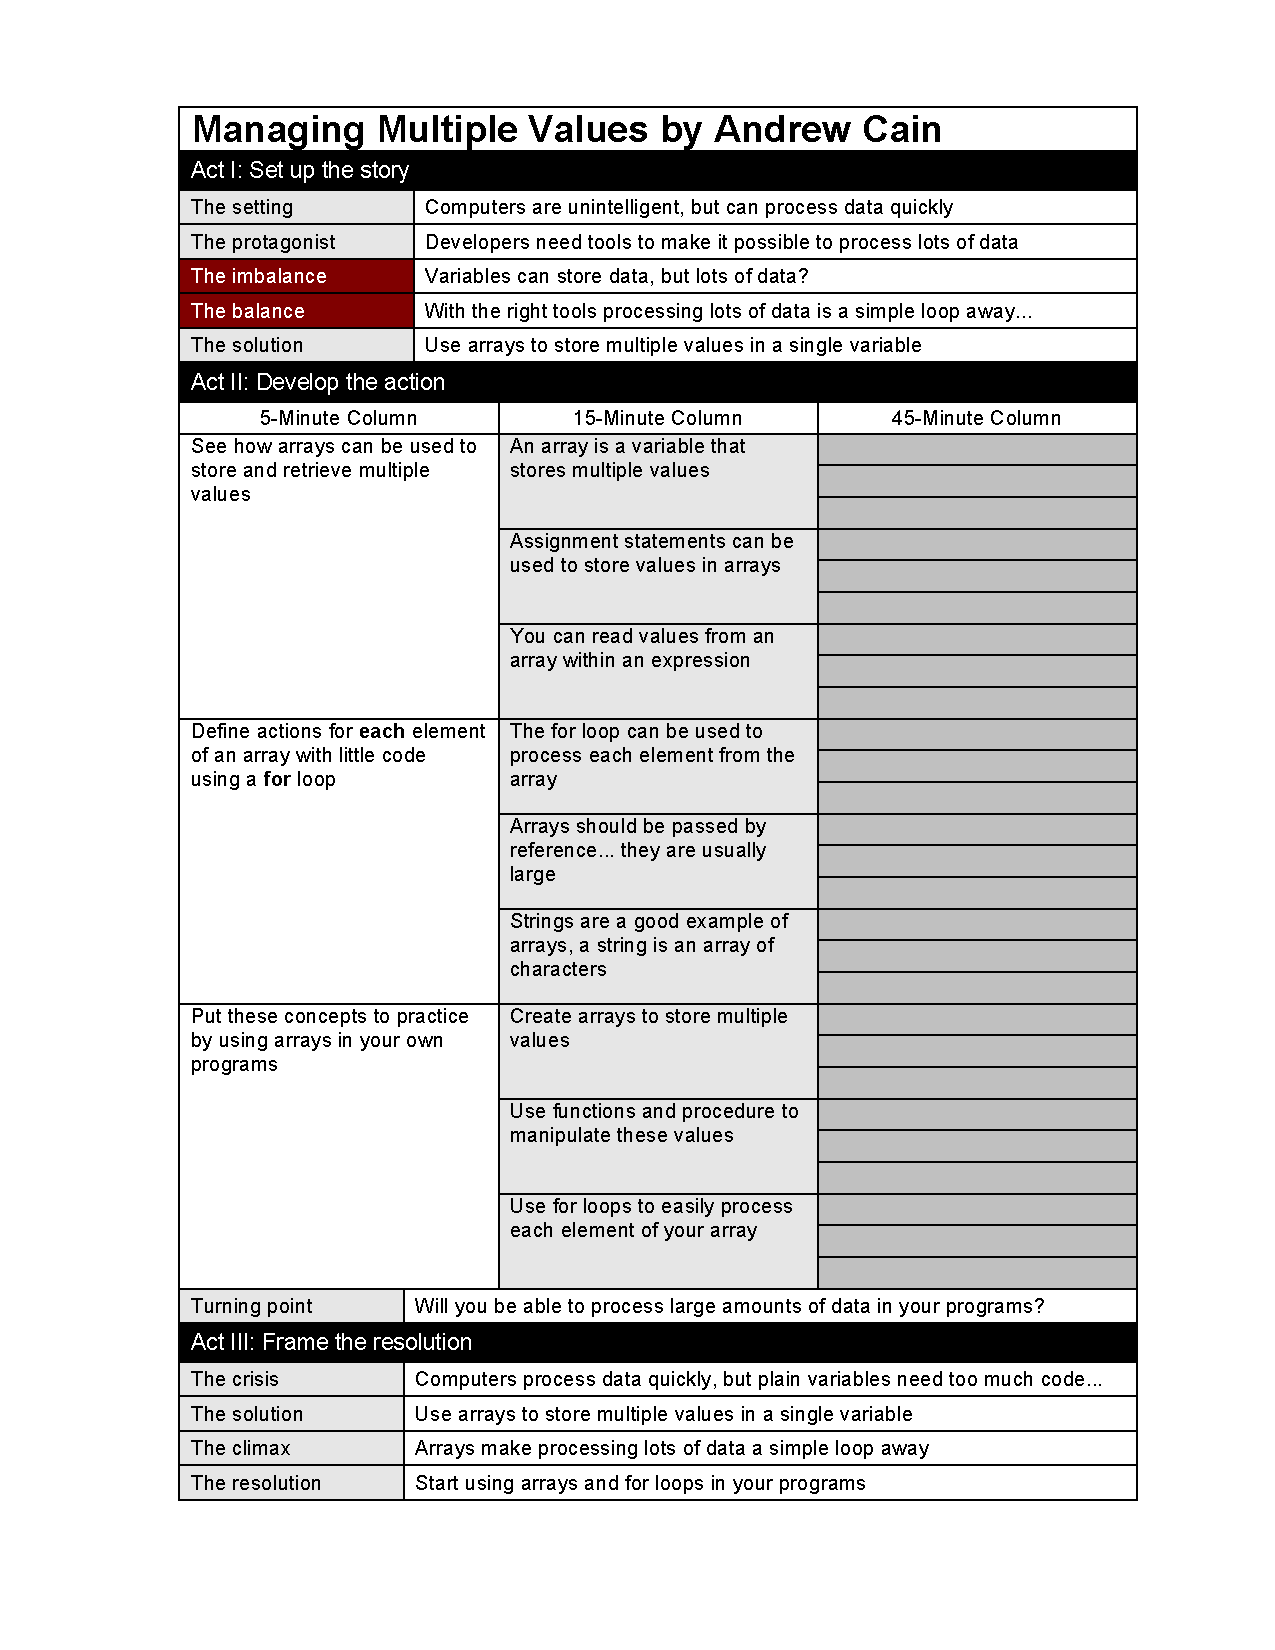
\includegraphics[width=\textwidth]{bbp}
	\caption{Example usage of the storyboard template, developed by \citet{Atkinson:2007} and available from \url{http://beyondbulletpoints.com}, that outlines the stages in a Beyond Bullet Points presentation.}
	\label{fig:bbp}
\end{figure}

The first five slides, termed Act 1, that set up the ``story'', telling the audience why they are there and centring them as the main character in the story. This helps motivate discussion, and focused teaching staff on clearly communicating the motivation behind the topic. The first five slides contain the following details:
\begin{enumerate}[label=Slide \arabic*:,labelwidth=*,align=left,noitemsep,nolistsep]
	\item \textbf{The setting}, sets the \emph{context}, positing the story at a relevant place within the content of the unit.
	\item \textbf{The protagonist} indicates the story is about the students, they are the focus not the teaching staff.
	\item Indicates \textbf{the imbalance}, stating a current problem, challenge or opportunity that motivates the need to find a solution.
	\item Juxtaposing the imbalance, \textbf{the balance} presents the goal, the situation in which the problem or challenge has been addressed, or the opportunity has been realised.
	\item Presents our \textbf{solution}, indicating how students (the protagonist) can get from the current \emph{imbalance} to the desired \emph{balance}.
\end{enumerate}

Slides contain a full sentence, written in an active voice. Ideally the slide text is accompanied by iconic visuals that set a theme or metaphor for the presentation. The time and resources necessary to prepare slides in this manner is, however, contrary to \pref{itm:agile}, being agile and willing to change these teaching and learning activities. If significant effort is spent developing slides in this way it is likely to increase resistance to change if adjustments to the topics message are desired. Instead, we suggest a minimalist approach with slides clearly showing the sentence text and using images to help communicate concepts central to the topic, as can be seen in the example slides shown in \fref{fig:lecture}.

For a fifteen minute presentation, the body of the presentation contained three main points, supported by three sub-points. Each addressed a ``why'' or ``how'' point, and supported the main solution. Once again these required a single short sentence in an active voice. The composition of these slides usually drew upon visuals created as part of the teaching and learning resources for the unit.

The last five slides conclude the presentation, reminding students of the overall solution and the new balance it brings about. These slides contain the following details:
\begin{enumerate}[noitemsep,nolistsep]
	\item The first slide in the conclusion was the \emph{turning point}. This is a question that asks a question of the students, indicating the presentation has turned to the conclusion. In effect it asks them if the concepts presented have shown them how to address the imbalance from the introduction.
	\item Next the \emph{crisis} slide restates the balance and imbalance, reminding the students of where the presentation started and where it was aiming to go.
	\item This then leads nicely to a restating of the \emph{solution}. This is an exact duplicate of the solution from the introduction, but now the student have been though the ``story'' and it should have more meaning.
	\item The \emph{climax} brings all of the pieces of the story together in summary and give the teaching staff a final opportunity to motivate students to study the topic further themselves.
	\item The final slide is the \emph{resolution}, and indicates the end of the presentation.
\end{enumerate}

Many of these guidelines from the Beyond Bullet Points approach were applied in the development of the lecture slides for the units discussed in \cref{cha:example_impl}. This included the general structure of the storyboard, though in some cases the three points were stretched to four but not beyond. The body of the presentations did include some information on ``what'' can be used, rather than purely focusing on ``how'' and ``why''. The use of active sentences, and visual communication, free from lists of bullet points, were also applied.

Focusing lecture slides in this manner helps to address the following principles from \cref{cha:guiding_principles}:

\begin{itemize}[noitemsep,nolistsep]
	\item Presentations aim to provide cognitive guidance, supporting students construction of knowledge. (\Pref{itm:construct})
 	\item Completing the story board requires a focus on the most important aspects for each topic. Where this focus is appropriately targeted, this also helps support alignment with intended learning outcomes. (\Pref{itm:align} and \Pref{itm:focus})
 	\item Shifting details from presentation to other resources requires a trust in students willingness to learn, supporting the need for a Theory Y attitude to motivation. (\Pref{itm:theory_y})
 	\item Using visuals for communicating core concepts, and minimalist themes for scaffolding slides, helps ensure presentations can be changed to respond to student needs. (\Pref{itm:agile})
 	\item The presentation style encourages a focus on concepts as little (if any) syntax would be used in the slides themselves. Instead, slides focus on visual representations to communicate programming concepts, leaving lower level details to be communicated via other means, as is discussed in \cref{cha:supporting}. (\Pref{itm:concepts})
 \end{itemize} 

\begin{figure}[htbp]
	\centering
	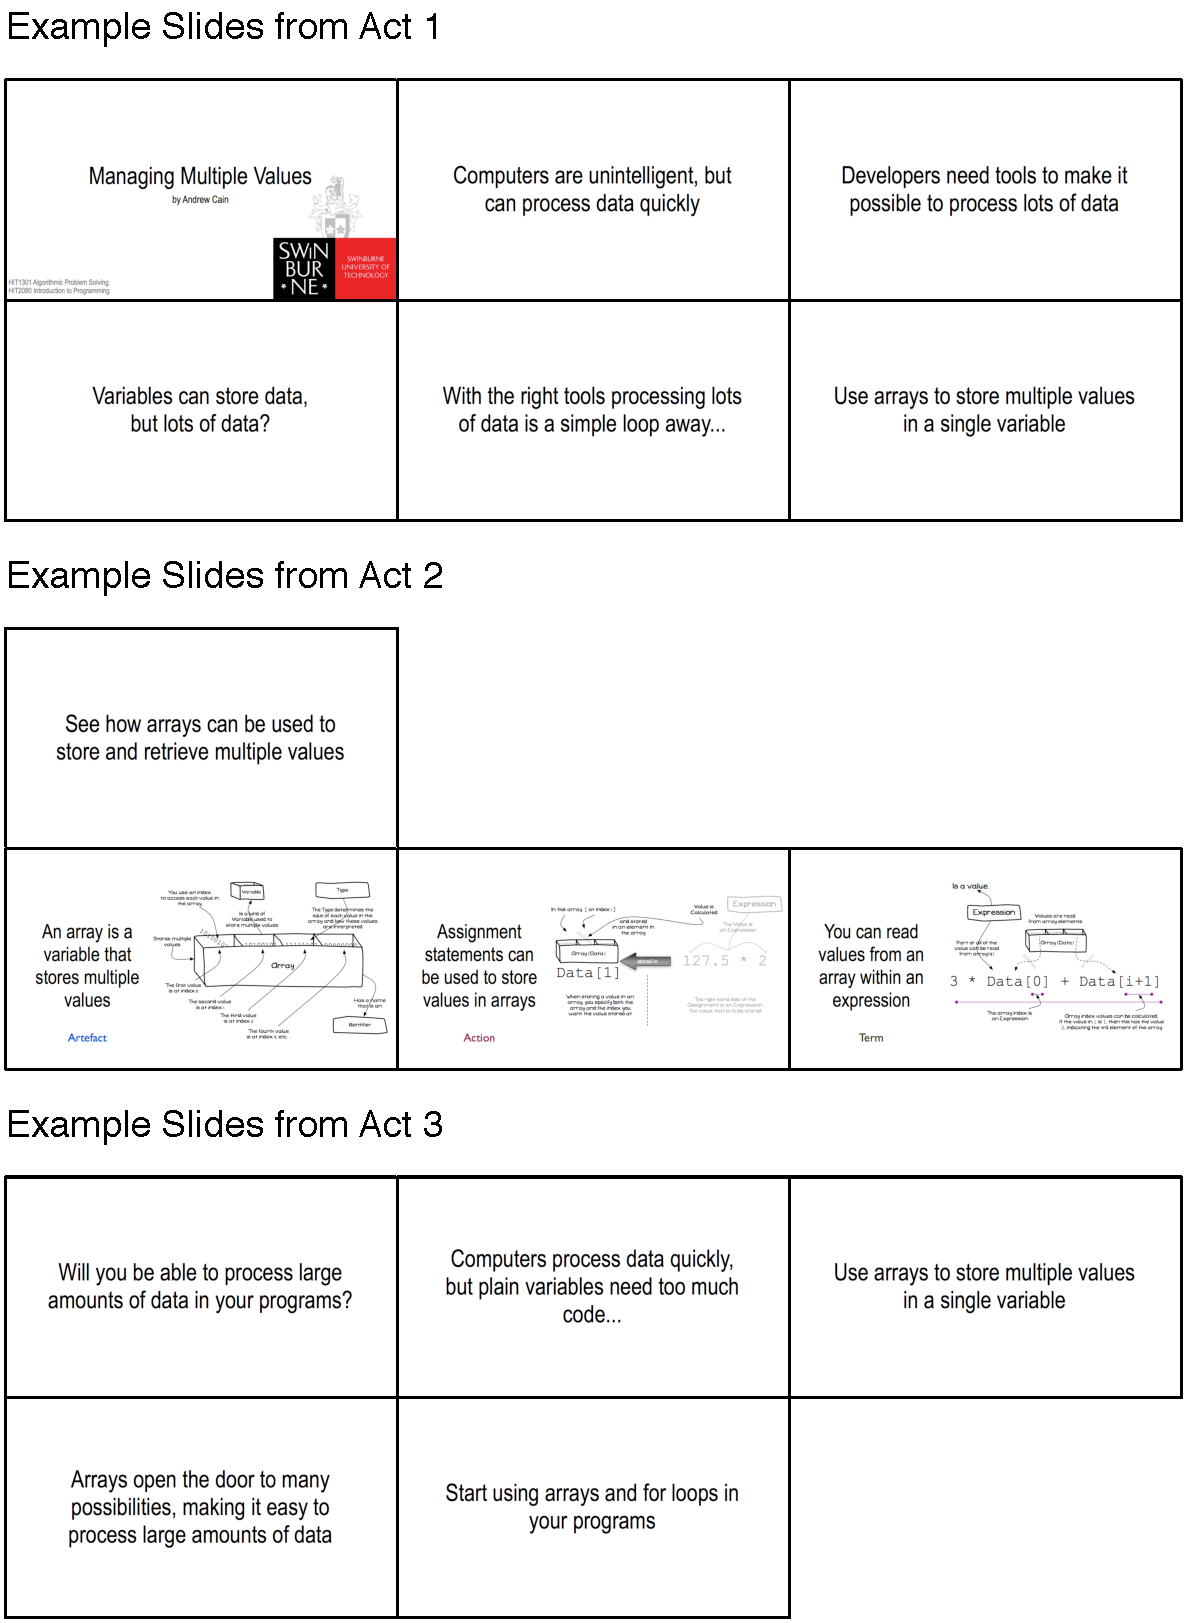
\includegraphics[width=\textwidth]{Lecture}
	\caption{Sample slides from the lecture created from the template shown in \fref{fig:bbp}. Act 1 and 3 use minimalist sentences, with visual representations of programming concepts being used to communicate the important concepts.}
	\label{fig:lecture}
\end{figure}

% subsubsection lectures (end)

\clearpage
\subsubsection{Interactive Lecture Demonstrations} % (fold)
\label{ssub:interactive_lecture_demonstrations}

Delivering one short, fifteen minute, presentation for each week's topic leaves a significant portion of a two hour lecture for other purposes. This time can be used to demonstrate the application of the concepts, providing students with a first experience of how these concepts can be used to create working programs. Similar approaches have been found to be an effective means of engaging students by \citet{Gaspar:2007} and \citet{Rubin:2013}.

The interactive sessions involve writing programs from scratch, guiding students through the whole software development process. This involves questioning students about what we should do, and which concepts we needed to apply. Program's are developed together with the students, enabling discussion as they evolve. This enables a focus on the thought processes behind program creation, taking students through the decisions that need to be made in crafting the design of the program being creating.

One important strategy we applied in these interactive coding sessions was for staff to become selectively forgetful, typically forgetting the syntax related to the current concept, for example. In this way, staff had to make use of the resources available to the students to \emph{find} the necessary details. For example, when focusing on how to declare variables this could be achieved by saying ``We want to create a variable here, but I can not remember the syntax. Where could I look to find the syntax for this?'' This triggers a discussion, and enables staff to demonstrate how to locate the associated resources, and lookup the relevant sections. Switching back to the code would be another point to ``forget'' the syntax, ``So what do I type first?''. The aim of this is to demonstrate to the students how these resources could be used to learn the language's syntax. In essence, providing an example of how to solve problems.

Depending on the topic, lectures typically follow one of two formats. Either the presentation was delivered in its entirety and was followed by the interactive session, or the interactive session was interwoven with the presentation itself. These two strategies can be applied at different times throughout the teaching period, depending on the topic. 

Topics in the first part of a unit are likely to have the interactive sessions interwoven with presentations. At this stage each of the concepts was totally new to the students. Presentations focused entirely on concepts is likely to make the topic very abstract. By interweaving live coding demonstration with presentations we aim to address student apprehension about how concepts are realised in practice.

Later topics, which reinforce earlier concepts, are likely to benefit from progressing more quickly through the slides and using a longer interactive demonstration. This would have the benefit of allowing a wider range of concepts to be demonstrated in a single session.

The use of interactive lecture demonstrations helps to address the following principles from \cref{cha:guiding_principles}:

\begin{itemize}[noitemsep,nolistsep]
	\item These sessions help provide students with a demonstration of applying unit concepts, aiding them in the construction of their own knowledge. (\Pref{itm:construct})
	\item In introductory programming, many of the intended learning outcomes relate to applying programming concepts to the development of small programs. These demonstrations are, therefore, directly aligned with activities we expect students to be able to demonstrate by the end of the unit.  (\Pref{itm:align})
	\item Guiding students through the use of supporting resources helps keep the focus on the most important concepts, while also helping students learn how to use available resources. (\Pref{itm:focus}, \Pref{itm:support} and \Pref{itm:concepts}).
	\item Demonstrations also provide an opportunity to illustrate good programming practice, and to show students examples of programs they are expected to be able to create. (\Pref{itm:expectations})
	\item Incorporating student input into the live demonstrations helps to motivate students, and requires a willingness to adapt to student requirements and needs. (\Pref{itm:theory_y} and \Pref{itm:agile})
\end{itemize}


% subsubsection interactive_lecture_demonstrations (end)

\clearpage
\subsubsection{Laboratory Sessions} % (fold)
\label{ssub:laboratory_sessions}

Laboratory sessions provide an opportunity for students to try applying the concepts covered in the lecture classes themselves. To help structure these sessions we organised these tasks into three groups: 

\begin{description}[noitemsep,nolistsep]
	\item [Laboratory tasks] were designed to be a guided exercise that was to be completed in class, providing detailed instructions on how to approach the problems presented.
	\item [Core tasks] had to be completed and submitted for feedback, helping students to develop pieces they can include in their portfolios.
	\item [Extension tasks] provided students with optional exercises they could use to extend themselves, requiring greater levels of independence and a better understanding of the concepts.
\end{description}

Tutors guide students through each week's laboratory tasks. These tasks were designed to give students their first hands-on experience with each week's concepts. Laboratory notes provided detailed step-by-step instructions to enable students to work through these on their own if they wanted, or need, to. At the end of the laboratory exercises students should be sufficiently prepared to undertake the core tasks.

Students then apply their understanding of each weeks concepts to complete the core tasks. It is important that these tasks ask the students to perform actions related to the unit's intended learning outcomes, as these tasks will help them create evidence they can include in their portfolios. For example, this could include tasks such as creating one, or more, small programs, or performing code reading exercises that ask students to hand execute programs and explain the program's behaviour, or identify issues in the presented code. 

Core tasks also form an integrated part of the formative feedback process. Once these tasks are completed students submit this work for feedback. Staff can then assess the work, and provide guidance on identified issues, and highlight possible misconceptions. If the work has issues, it can then be returned to the student with instructions on what needs to be corrected. Students can then work to address these issues, and associated misconceptions, and resubmit the work at a later stage. Where the task has been performed to a sufficient standard it can be signed off as complete, indicating that the student appears to have understood the associated concepts.

Extension tasks provide students with extra activities they can perform each week to demonstrate a deeper understanding of the associated concepts. These tasks are typically loosely defined, requiring students to explore the concepts in a more independent manner. A range of challenging tasks can be provided to support different student interests, and to provide students with ideas for activities that are likely to help them create pieces that will demonstrate valuable learning in their portfolios.

Laboratory sessions are highly student-centred, so organising these sessions in this way helps to address many of the principles from \cref{cha:guiding_principles}.  

\begin{itemize}[noitemsep,nolistsep]
	\item Activities help students develop their knowledge of the concepts being covered. (\Pref{itm:construct}) 
	\item Staff help ensure that these tasks relate to the unit's intended learning outcomes, ensuring students will be able to demonstrate how they have met these outcomes when they submit their portfolios. (\Pref{itm:align})
	\item Core tasks are used to provide students with formative feedback during the semester. (\Pref{itm:formative})
	\item Students are able to focus on the most important aspect for them at their current stage of development. Laboratory tasks focus on getting students started, core tasks focus on problems that demonstrate passable knowledge, while extension tasks can support the demonstration of more advanced levels of understanding. (\Pref{itm:focus})
	\item The formative process, with changes to core tasks being required before they are signed off, helps to clearly communicate the high standard expected of students. This is further supported by the list of extension tasks provided each week. These communicate the extra tasks the students \emph{should} be completing to demonstrate a deeper understanding of the concepts. (\Pref{itm:expectations})
	\item The different laboratory task levels each provide support for students at different stages of capability, while options in the extension tasks also help to support a range of student interests. (\Pref{itm:support})
	\item Using this approach students take a greater responsibility for their own learning. (\Pref{itm:theory_y})
\end{itemize}

% subsubsection laboratory_sessions (end)
% subsection content_approach (end)

\clearpage
\subsection{Summary} % (fold)
\label{sub:summary}

The overall strategy is defined by two approaches: the assessment approach, and the approach to content selection. Decisions related to these two approach were guided by the principles from \cref{cha:guiding_principles}, and resulted in the selection of a \textbf{portfolio assessment} approach to units that are taught using a range of student-centred teaching and learning activities. \fref{fig:overall_strategy} shows an updated version of \fref{fig:strategy}, showing the selected approaches discussed in this section. The next section describes the model for constructive alignment that developed from this overall strategy.

\begin{figure}[hb]
	\centering
	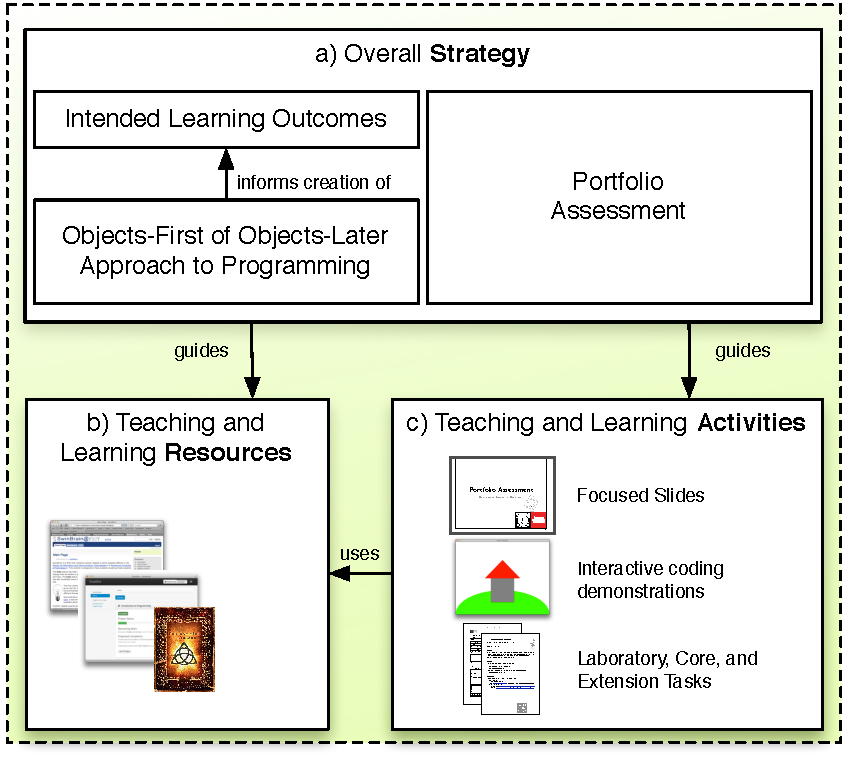
\includegraphics[width=0.8\textwidth]{OverallStrategy}
	\caption{An updated version of \fref{fig:strategy} showing the selected assessment approach, and the interactive teaching and learning activities.}
	\label{fig:overall_strategy}
\end{figure}

% subsection summary (end)
% section overall_strategy (end)
\clearpage
\section{Constructively Alignment with Portfolio Assessment} % (fold)
\label{sec:model}



\subsection{Model Overview} % (fold)
\label{sub:model_overview}

Having decided upon an overall strategy, the next stage of our research was to determine how Biggs' model of constructive alignment~\cite{Biggs:1996c}, and the details on using portfolio assessment suggested by \citet{Biggs:1997}, could be used to guide the creation of an introductory programming unit. This involved the examination of the practical advice from \citet{Biggs:2007}, which further elaborates on Biggs' model of constructive alignment and portfolio assessment. Using this together with the principles from \cref{cha:guiding_principles}, a model of constructive alignment for introductory programming was defined. The resulting model was documented in \citet{Cain:2012a}, and captured staff and student processes and the artefacts generated and exchanged throughout the learning process, as illustrated in \fref{fig:process_overview}.

\begin{figure}[htbp]
	\centering
	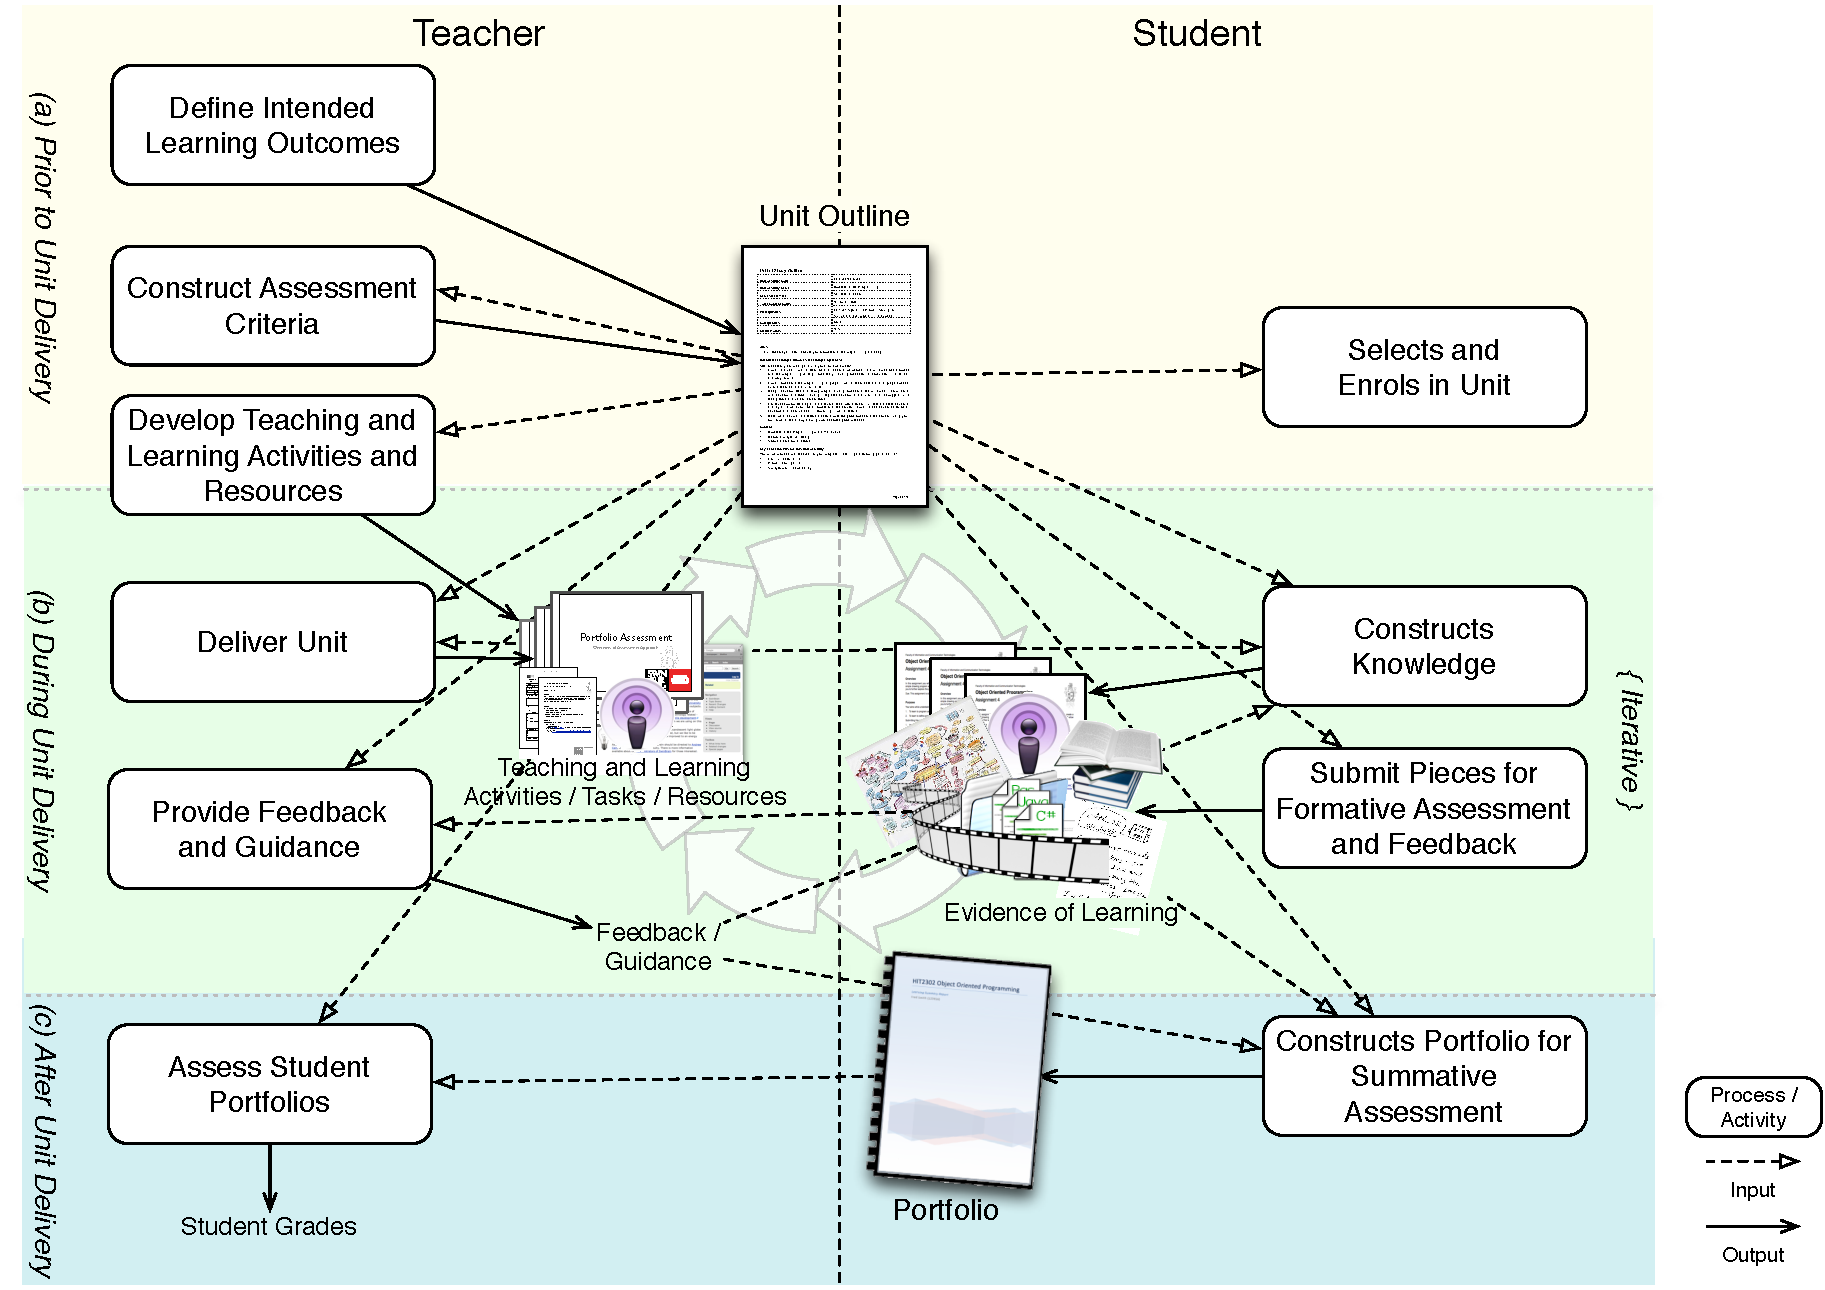
\includegraphics[width=\textwidth]{ProcessOverview}
	\caption{An overview of teacher and students roles (columns), and iterative delivery, in the constructive alignment model developed for the introductory programming units.}
	\label{fig:process_overview}
\end{figure}

Processes within the model are performed either by \emph{students} or \emph{teaching staff}. These processes are distributed across three stages of unit development and delivery: being either \emph{prior} to the start of the teaching period, \emph{during} the teaching period, or \emph{after} the teaching period. \fref{fig:process_overview} illustrates this with separate columns for teaching and student processes, and rows for the stages in which these processes occur.

Prior to the start of the teaching period (a) the teaching staff \emph{define intended learning outcomes} and \emph{construct assessment criteria}. Together these aspects form a critical component of unit, defining what students will be able to achieve after successfully completing the unit, and how well they must perform in order to achieve different grade outcomes. Both the intended learning outcomes and assessment criteria are documented in the Unit Outline, a document that is a common practice in university environments. The Unit Outline forms the central focus for subsequent processes, and informs and guides staff in the \emph{development of teaching and learning activities}. Unit outlines may also be used by students in evaluating units to select in their course of study.

The developed teaching and learning activities and their associated resources are then used during the teaching period (b) by staff to \emph{deliver the unit}. Students follow the guidance of teaching staff, and ideally these activities aid students as they \emph{construct knowledge}. The work that students produce can then be \emph{submitted for formative feedback}, which provides an opportunity for teaching staff to \emph{provide feedback and guidance}. The process of students undertaking activities, constructing knowledge, and receiving formative feedback is designed to be an ongoing iterative process throughout the teaching period.

After the conclusion of the teaching period (c) students prepare their work for summative assessment through the \emph{construction and submission of their portfolios}. These portfolios are then \emph{assessed by} the teaching staff against the intended learning outcomes and assessment criteria prepared prior to the unit's delivery.

Each of these processes is described in more detail in the following section.

% subsection model_overview (end)

\subsection{Processes within the Model} % (fold)
\label{sub:processes_within_the_model}

\subsubsection{Defining Intended Learning Outcomes} % (fold)
\label{sub:defining_intended_learning_outcomes}

Intended learning outcomes are central to the concept of constructive alignment as a statement of what students will be able to achieve at the end of the unit. Aligned curriculum in constructive alignment indicates that teaching and learning activities and assessment must \emph{align} to these intended learning outcomes. The findings in \cref{cha:background} indicate that alignment is typically performed by staff who indicate how teaching and learning activities and assessment tasks are aligned. Alignment is a matter external from the actual teaching itself. There is little involvement of the student in this process.

With portfolio assessment the alignment becomes intrinsically entwined with unit delivery and assessment. The teaching staff relinquish control of this aspect and the outcomes themselves take on their true purpose: as a statement of what students will be able to achieve at the end of the unit. All other aspects of the unit must now align to this purpose. Teaching and learning activities must prepare students to demonstrate that they have achieve these outcomes. Assessment aims to verify the extent to which students have reached these outcomes.

One way to conceptualise the central role of the intended learning outcomes is to picture this situation as a very long examination. The intended learning outcomes are the questions, the things students need to demonstrate they can do by the end of the ``exam''. The intended learning outcomes have become the assessment, a direct realisation of the fact that ``assessment always drives the curriculum'' \cite{Ramsden:2003}.  In this arrangement there is little opportunity for misalignment between the unit objectives and assessment, but a greater importance on the exact nature of the intended learning outcomes. This critical role of the intended learning outcomes means that they are instrumental in the success of the unit. 

For the introductory programming units it was important to design the intended learning outcomes so that, as a group, they cover the required programming competencies as well as the associated conceptual knowledge. The intended learning outcomes play a central role in driving the processes of both students and teaching staff. As a result, it is important they are expressed clearly and simply so as to be understood by all involved.

Development of unit outcomes has a variety of input sources. \citet{Thota:2010} propose inputs related to pedagogic theory (constructivism and phenomenography) as well as student factors such as approach to learning, learning styles, and prior knowledge. \citet{Armarego:2009} highlights the needs for inputs from industry, such as the Computer Science and Software Engineering Curriculum from professional standards bodies and associated Bodies of Knowledge \citet{Abran:2001}. For curriculum recommendations from professional standards bodies see \citet{Lethbridge:2006}, \citet{Cassel:2008}, and \citet{CSC2013}.

In defining the intended learning outcomes for an introductory programming unit using constructive alignment with portfolio assessment we suggest drawing upon these sources, as well as the guiding principles from \cref{cha:guiding_principles}, overall strategy, resourcing factors, and accreditation requirements as shown in \fref{fig:defining_ilos}. Resourcing factors provide additional constraints on what intended learning outcomes can include. Factors such as staffing, availability of texts, required tools, and others all need to be considered to ensure that students will be able to engage in activities associated with demonstrating the expected outcomes. Accreditation standards, such as the Australian Qualifications Framework \cite{AQF:2013}, require intended learning outcomes to demonstrate certain levels of achievement in order for degree programmes to gain recognition and funding. As these units will form an important part of programme objectives, these requirements must also be considered. 

\citet{Biggs:2007} provided a number of recommendations for the development of intended learning outcomes. They indicated that it was appropriate for a unit to have between four and six intended learning outcomes, expressed at suitably high cognitive levels. Adopting this approach enables the clear focus on what is important for the unit, and encourages depth over breadth, \pref{itm:focus} from \cref{cha:guiding_principles}. A small number of intended learning outcomes keep the focus clear for students.

% removed SOLO details from here...

As discussed in \cref{cha:background}, the SOLO Taxonomy proposed by \citet{Biggs:1982} provides a framework for ensuring intended learning outcomes aim for suitably high cognitive levels. Each of the identified cognitive levels has an associated list of verbs likely to elicit that level of activity. \tref{tbl:solo_verbs} lists selected verbs associated with the various levels of the SOLO taxonomy. These verbs can be used when defining the unit's intended learning outcomes. Biggs suggests that intended learning outcomes for university level units should aim for at least the multistructural level, with many units aiming for understanding at the relational level. In a review of science curricula in Danish universities, \citet{Brabrand:2009} argued that the SOLO taxonomy provided a good tool for specifying competency with a range of areas showing progressing depth in terms of SOLO verbs from undergraduate to graduate education.

\begin{figure}[p]
	\centering
	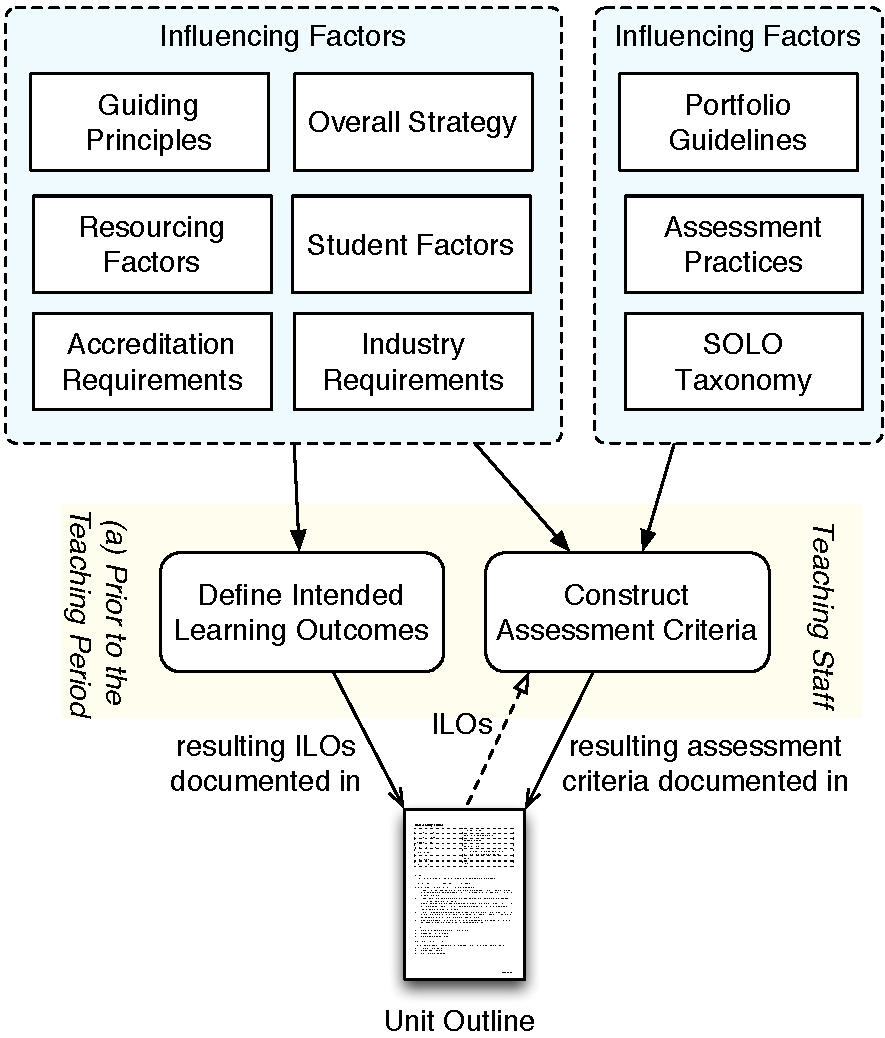
\includegraphics[width=0.55\textwidth]{DefiningILOs}
	\caption{Factors that influence the defining of a unit's intended learning outcomes, and the construction of assessment criteria. These activities are undertaken by teaching staff prior to the start of the teaching period, see (a) from \fref{fig:process_overview}. }
	\label{fig:defining_ilos}
\end{figure}

\begin{table}[p]
	\renewcommand{\arraystretch}{1.6}
	\centering

	\caption{Selected list of verb related to the levels of the SOLO Taxonomy suitable for defining intended learning outcomes, adapted from \citet{Biggs:2007}.}
 	\label{tbl:solo_verbs}
 	\footnotesize
    \begin{tabular}{lp{10cm}}
    SOLO Level        & Verbs likely to elicit indicated cognitive level \\
    \hline
    \textbf{Unistructural}     & memorize, identify, recognise, count, define, draw, find, label, match, name, quote, recall, recite, order, tell, write, imitate\\
    \textbf{Multistructural}   & classify, describe, list, report, discuss, illustrate, select, narrate, compute, sequence, outline, separate\\
    \textbf{Relational}        & apply, integrate, analyse, explain, predict, conclude, summarise, review, argue, transfer, plan, characterise, compare, contrast, differentiate, organise, debate, make a case, construct, review and rewrite, examine, translate, paraphrase, explain causes \\
    \textbf{Extended Abstract} & theorise, hypothesise, generalise, invent, originate, make original case\\
    \end{tabular}
\end{table}

We developed the following guidelines that can be used to inform the formation of the intended learning outcomes for portfolio assessed programming units.

%
% Can these "principles" be linked back to the Ch 3 ones??
% 
%
% I wonder about the use of "principle" in the context of both chapters?
% I wonder if the following (and in the following sections this chapter) could
% be renamed as something else e.g. guidelines?
% AC: renamed to guidelines
%
% Do you need/want to number these e.g.LO-1, LO-2 for "Learning Outcome guidelines"
% to refer to from Ch5 ??? 
%

\begin{itemize}[noitemsep,nolistsep]
  \item Express outcomes using verbs at an appropriate level of understanding with reference to the SOLO taxonomy.
  \item Cover both the required \emph{conceptual knowledge}, and \emph{programming competencies}.
  \item Use \emph{simple terms} (where possible) to communicate outcomes, thereby helping to ensure they can be understood by all students undertaking the unit.
  \item The number of outcomes should be \emph{minimal}, ideally between four and six. This is to help ensure that each outcome covers a meaningful body of knowledge to a sufficient depth.
  \item Outcomes need to be \emph{general} to facilitate assessment of diverse portfolios, and \emph{sufficient} to ensure that differing degrees of proficiency and understanding can be assessed.
  \item There needs to be \emph{flexibility} to enable students to choose a range of means when addressing outcomes.
\end{itemize}

Developing intended learning outcomes in this way helps to address the following principles from \cref{cha:guiding_principles}:
\begin{itemize}[noitemsep,nolistsep]
	\item Stated outcomes become the goal students work toward throughout the teaching period. Ensuring these are expressed using appropriate verbs from the SOLO taxonomy ensures they are likely to engage appropriate cognitive levels. (\Pref{itm:construct} and \Pref{itm:align})
	% \item (\Pref{itm:formative})
	\item Keeping the list of objectives short help ensure they are focused on the concepts related to the unit. (\Pref{itm:focus} and \Pref{itm:concepts})
	\item Using verbs from the relational level of the SOLO taxonomy helps communicate staff expectations. (\Pref{itm:expectations})
	\item Ensuring flexibility and clarity helps support a wider range of student interests and capabilities. (\Pref{itm:support})
	% \item (\Pref{itm:theory_y})
	% \item (\Pref{itm:agile})
	% \item (\Pref{itm:reflect})
	% \item (\Pref{itm:paradigm})
	% \item (\Pref{itm:authentic})
\end{itemize}





% subsection processes_within_the_model (end)
\subsubsection{Constructing Assessment Criteria} % (fold)
\label{sub:constructing_assessment_criteria}

Assessment criteria are developed alongside the definition of intended learning outcomes. The intended learning outcomes state what students need to demonstrate by the end of the unit, but these outcomes can be achieved to different standards. It is the role of the assessment criteria to state the required level of achievement students must demonstrate in order to be awarded various grade outcomes. This means that at the end of the teaching period students' portfolios can be assessed against the developed assessment criteria, but also that the assessment criteria can be used to guide the teaching and learning activities during delivery. Providing assessment criteria in the unit outline creates a simplified learning contract \cite{Stephenson:1993}, in which students know ``up front'' what is required to achieve the different grades. 

\pref{itm:formative} indicates that assessment should judge outcomes. To provide this holistic judgement the final summative assessment is \emph{criterion-referenced}, as suggested by \citet{Biggs:1997}. The criteria must, therefore, provide a means for teaching staff to assess submitted portfolios while also providing students with guidance they can use during the delivery and in the construction of their portfolios. Ensuring that the assessment criteria are stated clearly also helps ease students transition to this new form of assessment \cite{Smith:2001}.

There is some contention regarding the specification of assessment criteria for assessing portfolios. For example, some consider that by overly specifying criteria students are limited in what can be included (see \citet{Driessen:2005} and \citet{Tigelaar:2007}). However, \citet{Smith:2001} indicated that clearly communicating portfolio requirements helped ease students transition to this new, possibly unfamiliar, assessment approach. This is further supported by \citet{Allan:1996}, who argued that clear communication of intended learning outcomes and assessment criteria enabled students to focus on developing knowledge required to succeed in a unit, and by \citet{Thorpe:2000} who noted that students found it easier to reflect on their learning if they were able to apply criteria defined by teaching staff.

The assessment criteria development process takes input from the intended learning outcomes, along with guidelines for portfolio assessment \cite{Biggs:2007} and levels of achievement from the SOLO taxonomy \cite{Biggs:1982} as shown in \fref{fig:defining_ilos}. The resulting criteria are placed alongside the intended learning outcomes in the unit outline.

In order to facilitate assessment, and to guide student activity, the assessment criteria need to indicate clearly distinct requirements for each grade outcome. In the university where this work was carried out there are five grade categories: Fail, Pass, Credit, Distinction and High Distinction. The assessment criteria indicate what students need to demonstrate to achieve each grade. 

The following list presents the assessment criteria developed in this work. The criteria are cumulative, with each level beyond pass requiring all previous requirements to be satisfied in addition to some deeper level of understanding being demonstrated. Pass requires that each intended learning outcome is met to a minimally acceptable standard, which will depend on the verb used in their description. Credit then requires an overall picture of the unit, with students starting to see how the various aspects of the unit come together as a whole. This is then required to achieve the Distinction grade, in which students must show they can apply unit concepts to the creation of a piece of work of their own invention. This does not need to be new or ``ground breaking'' work, just something the student created on their own that shows all of the intended learning outcomes in play. High Distinction then goes beyond this by asking students to engage is a small research project, encouraging them to work toward an extended abstract\footnote{Extended abstract requires a level of understanding where new knowledge can be created.} level of understanding, but not requiring that they achieve this.
\begin{description}[noitemsep,nolistsep]
	\item[Fail] is a result of anything less than Pass level.
	\item[Pass] demonstrates \emph{minimally acceptable} level of achievement. Students have been able to complete core tasks from the teaching and learning activities, and pass any hurdle\footnote{Hurdle requirements are anything that must be ``passed'' to pass the unit, but do not contribute marks toward the final grade.} requirements.
	\item[Credit] demonstrates all Pass requirements and shows a \emph{good} depth of understanding across all intended learning outcomes, but does not go beyond presented work. Demonstrates at least a multistructural level of understanding of the unit overall.
	\item[Distinction] demonstrates Credit level requirements and the ability to \emph{apply} unit concepts to the creation of work of the students own invention. This demonstrates at least a relational level of understanding of the unit overall.
	\item[High Distinction] demonstrates all Distinction level requirements and the ability to \emph{research} a topic related to the unit. This still requires only a relational level of understanding, but provides opportunities and encouragement for students to explore beyond the current knowledge and work toward that extended abstract level of understanding.
\end{description}

\clearpage 

The following guidelines were used to inform the definition and communication of the assessment criteria:

%
% Can these "principles" be linked back to the Ch 3 ones??
% 

\begin{itemize}[noitemsep,nolistsep]
  \item Communicate assessment criteria using \emph{simple terms} (as suggested for the outcomes).
  \item Require sufficient progress to be demonstrated for all intended learning outcomes. At least a multistructural level of understanding should be obtained for passing students.
  \item Higher grades should require:
  \begin{itemize}[noitemsep,nolistsep]
  	\item evidence of \emph{deeper learning}, while specifically avoiding an excessive volume of work.
  	\item integrated understanding across related intended learning outcomes, as well as within each intended learning outcome.
  \end{itemize}
  \item Aim to develop \emph{clearly distinct} assessment criteria for each grade outcome, facilitating timely assessment and providing clear requirements for students.  
  \item Clearly \emph{map assessment criteria} to grade outcomes, ensuring students and staff have a shared understanding of how a portfolio relates to final grades.
\end{itemize}

Constructing the assessment criteria using these guidelines helps to address the following principles from \cref{cha:guiding_principles}:

\begin{itemize}[noitemsep,nolistsep]
	\item Requiring progressively higher levels of understanding for each grade classification help promote deep learning, and indicates staff expectations in terms of required levels of demonstration. (\Pref{itm:construct} and \Pref{itm:expectations})
	\item Assessment criteria align to unit outcomes, with higher grades requiring students to demonstrate an understanding of the relationships between the intended learning outcomes and their associated concepts. (\Pref{itm:align} and \Pref{itm:concepts})
	\item Grades are awarded using criterion referenced assessment, assessing students' learning outcomes. (\Pref{itm:formative})
	\item Specific criteria help focus students on the most important aspects, with higher grades requiring demonstration of deeper learning. (\Pref{itm:focus})
	\item The use of simple terms help support a wide range of student language capabilities. (\Pref{itm:support})
	\item Students can take responsibility for their learning, being able to aspire to achieve a given grade, and being able to apply their own imagination and interests in applying concepts to achieve higher grades. (\Pref{itm:theory_y})
	\item Evidence from student submissions provide a source of evidence for change, and can be reflected upon at the end of each teaching period to inform future changes. (\Pref{itm:agile} and \Pref{itm:reflect})
	% \item (\Pref{itm:paradigm})
	% \item (\Pref{itm:authentic})
\end{itemize}



% section a_constructively_aligned_model_for_introductory_programming (end)

\clearpage
\subsubsection{Develop Teaching and Learning Activities and Resources} % (fold)
\label{ssub:develop_teaching_and_learning_activities_and_resources}

Having defined the intended learning outcome, and assessment criteria, teaching staff develop, or select, appropriate teaching and learning activities and resources. \fref{fig:develop_tlar} illustrates the role of this process in the overall unit delivery. The process uses inputs from the Unit Outline, and generates both teaching and learning activities and resources.

\begin{figure}[htbp]
	\centering
	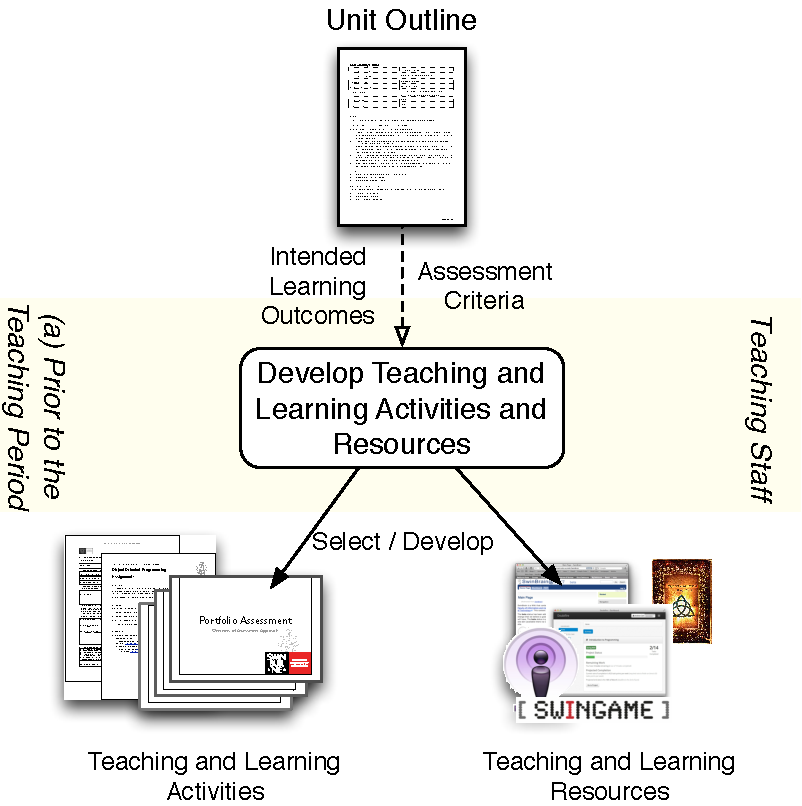
\includegraphics[width=0.6\textwidth]{DevelopTLAR}
	\caption{Development of teaching and learning activities and resources uses details from the unit outline to create/select appropriate resources and activities to ensure students engage appropriate activities during the teaching period.}
	\label{fig:develop_tlar}
\end{figure}

The teaching and learning activities aim to elicit appropriate behaviour from students, ensuring that they engage in the cognitive processes representative of the desired level of achievement for each intended learning outcome. Output generated from this process includes lecture slides and tutorial/laboratory handouts. In relation to the overall strategy, these activities are likely to change frequently as teaching staff become better able to direct student efforts. In keeping with our agile principles (\pref{itm:agile}) the effort spent on developing these teaching and learning activities should be minimised.

In contrast, teaching and learning resources provide students with detailed information they will require to successfully complete the teaching and learning activities. If designed appropriately, these resources should have a longer lasting value, and can change less frequently than the teaching and learning activities. Central to this approach is the idea of focusing (\pref{itm:focus}) each aspect of the teaching and learning environment to best benefit the construction of student knowledge (\pref{itm:construct}). Teaching and learning resources provide details, and extra attention and effort are required in their development, with the benefit of being able to be used in a range of contexts. Examples of resources include textual and visual illustrations, video podcasts showing example usage, online tools, and supportive software. Some of these resources can then be used in the creation of the lecture slides, but the lectures focus on providing cognitive guidance, directing students through the most important aspects with the details to be discovered later when students make use of the provided resources.

%
%Can these "principles" be linked back to the Ch 3 ones??
% 

The following guidelines were used to inform this process:

\begin{itemize}[noitemsep,nolistsep]
	\item Teaching and learning \textbf{activities} should:
	\begin{itemize}[noitemsep,nolistsep]
	 	\item Actively engage the students.
	 	\item Align with the unit's intended learning outcomes.
	 	\item Focus on providing guidance:
	 	\begin{itemize}[noitemsep,nolistsep]
		 	\item Lectures should inform, motivate and inspire students. Providing students with the key ingredients needed to get started with the tutorial/laboratory tasks.
		 	\item Tutorial/Laboratory tasks should direct students to perform activities that engage appropriate cognitive levels, helping them create artefacts that can be included in their portfolios.
	 	\end{itemize}
	 \end{itemize} 

	\item Teaching and learning \textbf{resources} should:
	\begin{itemize}[noitemsep,nolistsep]
		\item Provide the details students require to perform the tasks from the teaching and learning activities.
		\item Be created with a focus on re-usability.
		\item Support a range of different learning styles.
	\end{itemize}
\end{itemize}

Material developed using these guidelines address the following principles from \cref{cha:guiding_principles}:

\begin{itemize}[noitemsep,nolistsep]
	\item Aligning activities to intended learning outcomes ensures students develop appropriate knowledge related to the units concepts. (\Pref{itm:construct}, \Pref{itm:align}, and \Pref{itm:concepts})
	% \item (\Pref{itm:formative})
	\item Focusing these activities on appropriate cognitive levels helps direct student attention, and communicate staff expectations. (\Pref{itm:focus} and \Pref{itm:expectations})
	% \item (\Pref{itm:support})
	% \item (\Pref{itm:theory_y})
	\item Separating activities from resources helps enable activities to change. (\Pref{itm:agile})
	% \item (\Pref{itm:reflect})
	% \item (\Pref{itm:paradigm})
	% \item (\Pref{itm:authentic})
\end{itemize}

See \sref{sub:delivery_approach} for some example activities developed using these guidelines.


% subsubsection develop_teaching_and_learning_activities_and_resources (end)

\subsubsection{Iteratively Deliver Unit and Provide Feedback} % (fold)
\label{ssub:deliver_unit}

Constructive learning theories emphasise the active role of the learner in constructing knowledge. Our guiding principles are centred on this notion and adopt Biggs' pragmatic view of constructivism. The iterative, students centred, delivery process aims to embody Biggs' quote ``It's what the student does that counts.'' \cite{Biggs:1996c}, a statement that can be traced back to Tyler's quote, ``It is what he does that he learns, not what the teacher does'' \cite{Tyler:1969}.

Existing work on constructive approaches to teaching introductory programming provide some advice on designing and delivering student-centred teaching and learning activities. \citet{BenAri:1998,BenAri:2001} discussed the need for students to construct appropriate models of the computer. \citet{VanGorp:2001} described collaborative and constructive environments with the use of code walk-throughs, writing code, debugging and other activities. \citet{Thramboulidis:2003} presented a design-first approach to object oriented programming that focused on engaging students with object oriented design processes. \citet{Wulf:2005} reported strategies such as moving content from lectures to online video presentations. Similarly, the work of \citet{Thota:2010} also presented constructive approaches to teaching introductory programming that focused on group work, and the active role of the student.

\begin{figure}[p]
	\centering
	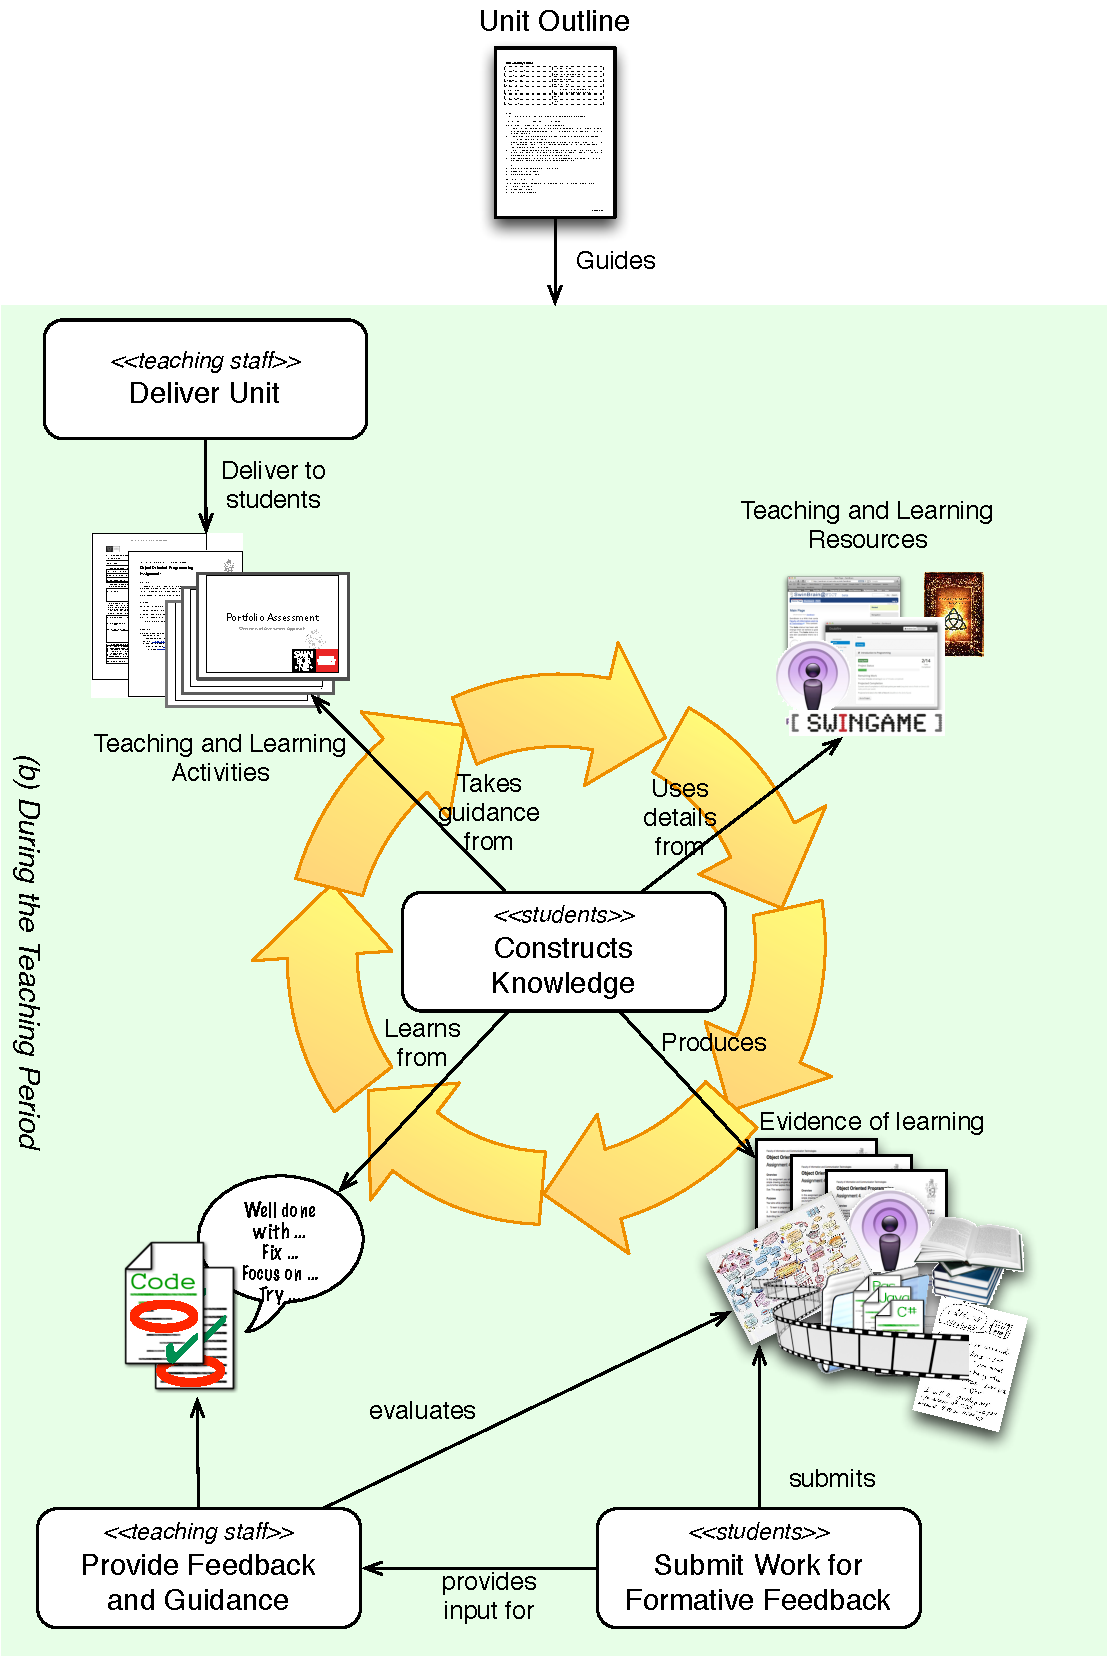
\includegraphics[width=0.8\textwidth]{DeliverUnit}
	\caption{Iterative nature of the unit delivery process}
	\label{fig:deliver_unit}
\end{figure}

\fref{fig:deliver_unit} illustrates the iterative delivery process at the heart of the model presented. The process centres on the students construction of knowledge, which draws up the teaching and learning activities and resources. This active process of learning generates pieces of work that the student submits for formative feedback. The teaching staff evaluate the evidence presented, trying to identify issues with the students current mental models, and provide formative feedback to the student. This feedback helps inform the student of their progress, and provides them with tasks they can act up thereby ensuring we close the loop.

All of these processes occur on a weekly basis, with rapid iteration ensuring feedback is timely and gives students the best chance of addressing misconceptions before the end of the teaching period. Each week, students will:

\begin{enumerate}[noitemsep,nolistsep]
	\item Attend lectures which guide them in relation to key aspects and motivations.
	\item Undertake set tasks from tutorial handouts, while drawing upon teaching and learning resources for required details.
	\item Produce work and submit for feedback.
	\item Receive feedback aimed to help them improve, and a list of changes required to meet the expected standard.
\end{enumerate}

For any one topic, this iterative process may take a couple of iterations before the student is successful in getting the work signed off. \fref{fig:construct_knowledge} is an illustration shown to students to indicate the iterative nature of the submission process. The highly connected nature of the topics in introductory programming means that it is critical students understand earlier topics before they move on. Work that is submitted is not considered complete by teaching staff until it demonstrates certain levels of understanding. While this is not the case, students need to correct and resubmit the work.

\begin{figure}[p]
	\centering
	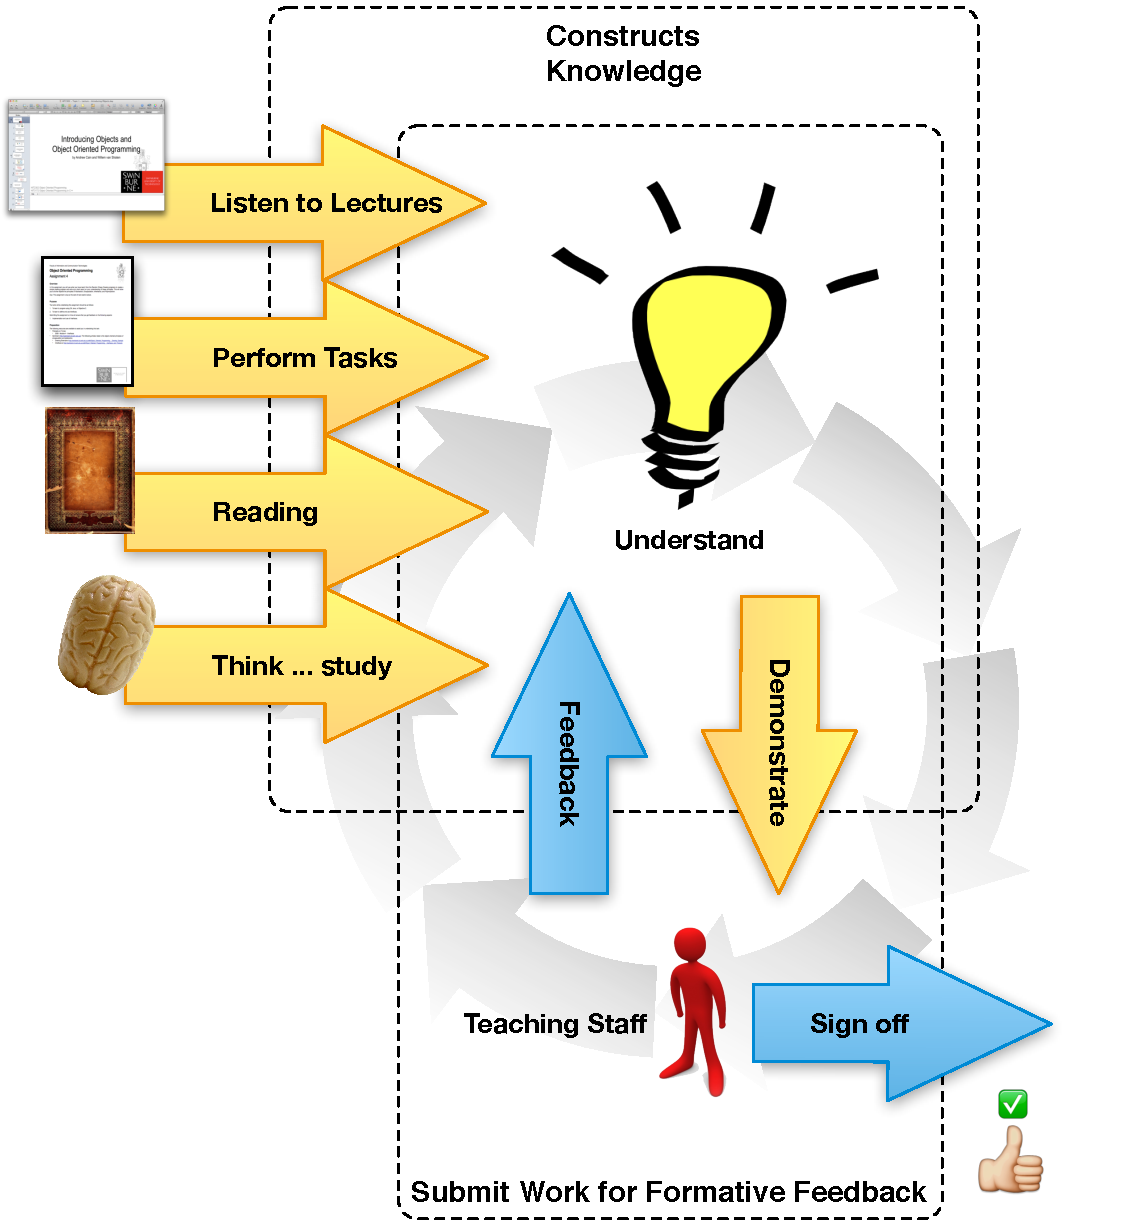
\includegraphics[width=0.9\textwidth]{ConstructKnowledge}
	\caption{Iterative process students undertake to get work signed off.}
	\label{fig:construct_knowledge}
\end{figure}

Requiring students to resubmit work ensures that no topic is half done. This focus on quality, and depth of understanding, helps communicate the high standards expected of students, \pref{itm:expectations}. Students are expected to submit some work for assessment each week. To enable fast turn around, this work is required in hard copy at the start of each week's lecture. This work is then evaluated by the teaching staff \emph{before} that week's tutorial classes (in practice 1 to 2 days). In the tutorial classes the work is returned to students, and the teaching staff briefly discuss progress with each student and the aspects of their work they can improve upon. This dialogue focuses on the student's individual understanding, and their demonstration thereof.

The following guidelines were developed and used to inform the planning and delivery of teaching and learning activities:

%
% Can these "principles" be linked back to the Ch 3 ones??
% 

\begin{itemize}[noitemsep,nolistsep]
  \item Provide opportunities through activity design to actively engage students -- \emph{it is what the student does that counts}.  
  \item Relate all activities to the objectives, providing students with opportunities to create evidence for their portfolio.
  \item Use ungraded formative feedback to aid knowledge construction, with preference for small, frequent guidance.
\end{itemize}

Adopting these guidelines in the delivery of a unit will help address the following principles from \cref{cha:guiding_principles}:

\begin{itemize}[noitemsep,nolistsep]
	\item Frequent formative feedback aids students' construction of knowledge, and helps ensure learning aligns with unit outcomes and concepts. (\Pref{itm:construct}, \Pref{itm:align}, \Pref{itm:formative} and \Pref{itm:concepts})
	\item Feedback can focus on the most important aspects, ensuring it is relevant to each student and their current level of understanding. (\Pref{itm:focus} and \Pref{itm:agile})
	\item Requiring work to be completed to a good standard helps reinforce staff expectations, and supports students by encouraging reflection and deep approaches to learning. (\Pref{itm:expectations}, \Pref{itm:support}, and \Pref{itm:reflect})
	\item Using formative feedback, without the marks associated with summative assessment, requires a Theory Y attitude to student motivation. (\Pref{itm:theory_y})
	% \item (\Pref{itm:paradigm})
	% \item (\Pref{itm:concepts})
	% \item (\Pref{itm:authentic})
\end{itemize}

% subsubsection deliver_unit (end)

\subsubsection{Construction, Submission, and Assessment of Portfolios} % (fold)
\label{ssub:construction_submission_and_assessment_of_portfolios}

The final phase of the process is the development and submission of portfolios by students, and assessment by staff. This process uses the intended learning outcomes and assessment criteria from the Unit Outline to determine what needs to be demonstrated and assessed. \fref{fig:portfolio_processes} illustrates the processes for portfolio construction by students, and assessment by staff. Students construct their portfolios from work completed during the teaching period. This work can incorporate feedback received, enabling students to showing off their best work and providing them with encouragement to act upon the feedback. \fref{fig:portfolio_pieces} shows an illustration used to explain the portfolio construction process to students. 

In preparing the portfolio, students must demonstrate that they have met all of the unit's intended learning outcomes. This alignment is documented by students in a \emph{Learning Summary Report}. The Learning Summary Report starts with a self assessment, in which the student indicates which grade they are \emph{applying} for with this portfolio. In the following sections students provide justification for why they should be awarded this grade. Students are required to list the pieces of work they have includes, and then explain how these pieces demonstrate that the student has attained all intended learning outcomes. The report ends with a reflection in which the student is encouraged to reflect upon the significance of what they have learnt, as well as on the process of learning itself. This learning summary report is then combined with the other pieces of work, printed, bound and submitted for assessment.

\begin{figure}[p]
	\centering
	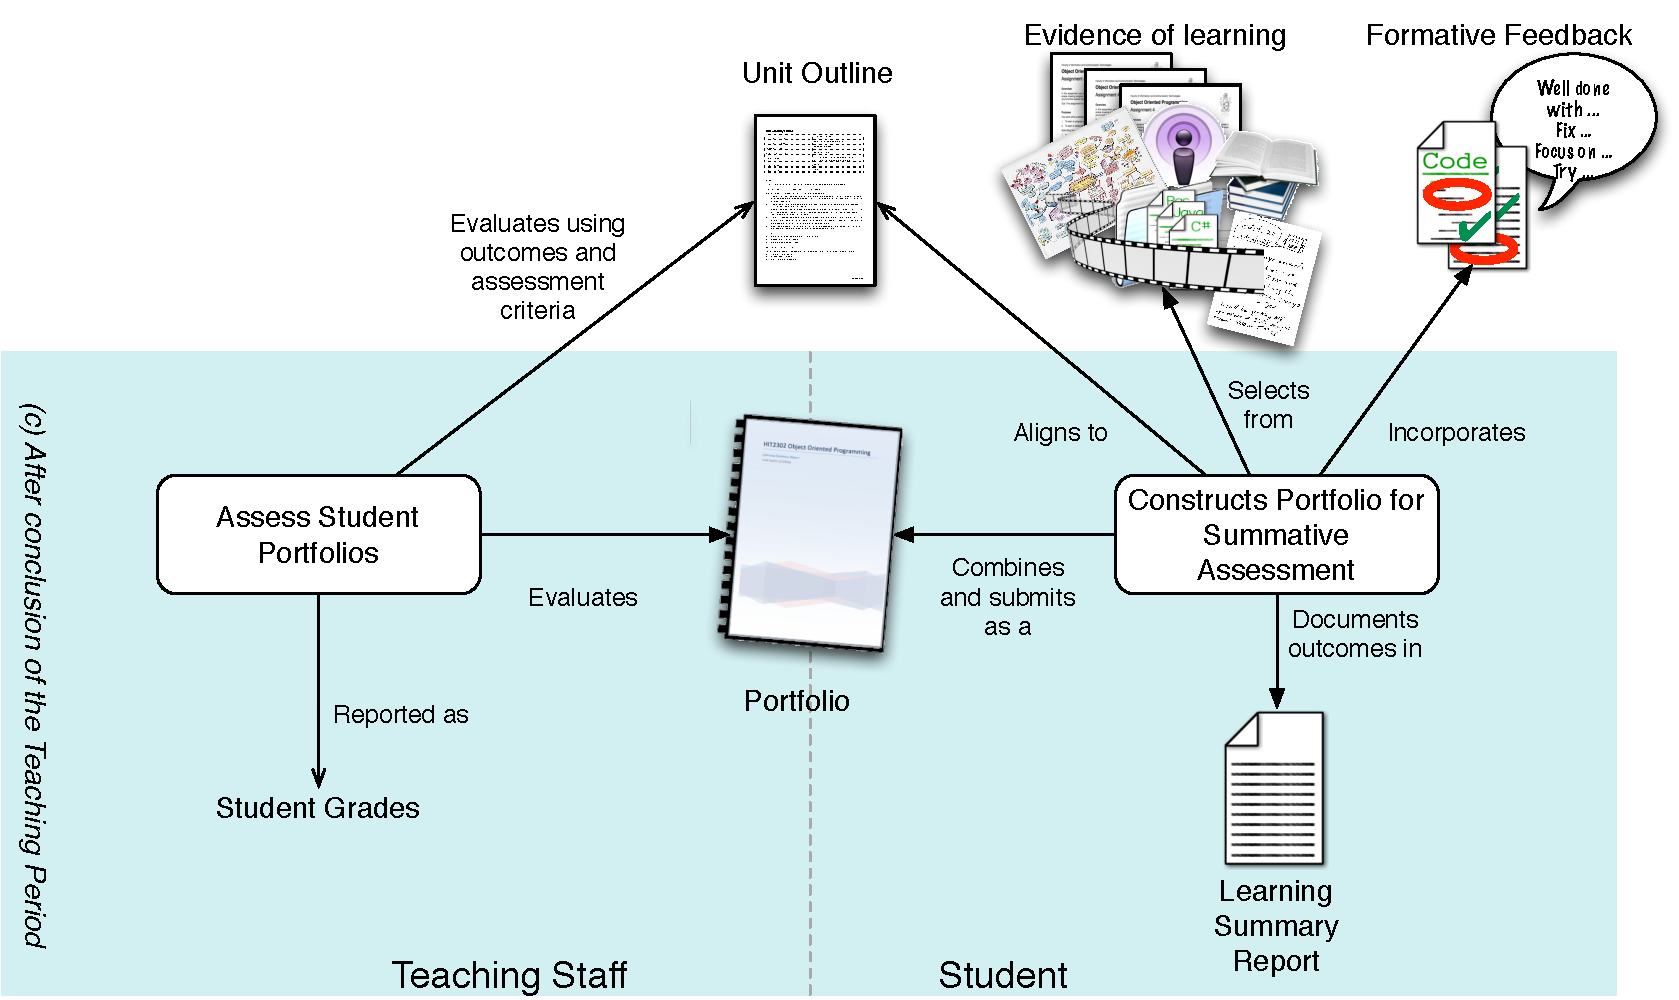
\includegraphics[width=\textwidth]{PortfolioConstructionAssessment}
	\caption{Processes of constructing, submitting, and assessment portfolios.}
	\label{fig:portfolio_processes}
\end{figure}

\begin{figure}[p]
	\centering
	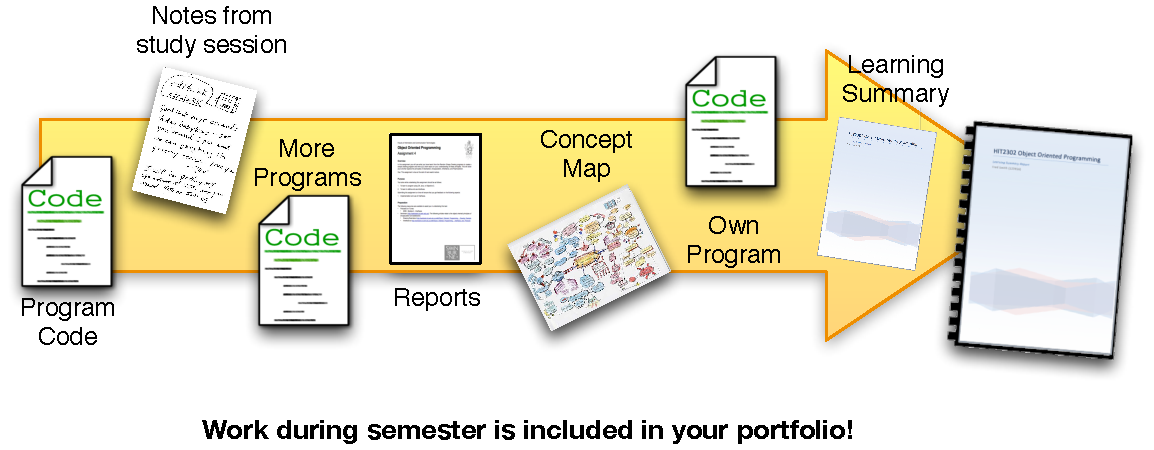
\includegraphics[width=0.9\textwidth]{PortfolioPieces}
	\caption{Illustration shown to students to highlight the process of constructing their portfolio during the teaching period}
	\label{fig:portfolio_pieces}
\end{figure}

The submission process differs based upon the grade students are aiming for in their portfolios. Students aiming for a Pass or Credit grade submit their portfolio by a set date in the examination period. These portfolios contain primarily work set out in the teaching and learning activities (``core'' tasks), and will have been checked already by teaching staff throughout the teaching period as part of the formative feedback process. Students aiming for Distinction or High Distinction are required to present their portfolio at an interview. In this interview students outline their custom work, and discuss how this relates to the unit's intended learning outcomes. The interviews are conducted in an open, relaxed, and friendly manner, and students are encouraged to elaborate on what they have achieved.

\clearpage
Based on our experience we suggest the following guidelines be used to inform the creation and assessment of portfolios:

%
% Can these "principles" be linked back to the Ch 3 ones??
% 

\begin{itemize}[noitemsep,nolistsep]
  \item Encourage unique, diverse, concise, and strongly aligned evidence.
  \item Motivate students to include evidence of learning from formative experience.
  \item Accurately and consistently follow the terms of the assessment criteria, as this is the \emph{contract} the students work towards.
  \item Require students to reflect on their learning, and the evidence in their final portfolio, with respect to the intended learning outcomes of the unit and the assessment criteria.
  \item Use an interview, or hurdle test(s), to check for minimal pass criteria in an invigilated manner. Where tests are used they need only distinguish between Pass and Fail, and do not need to address higher grades. 
\end{itemize}

Applying these guidelines to the creation and assessment of portfolios helps address the following principles from \cref{cha:guiding_principles}:

\begin{itemize}[noitemsep,nolistsep]
	\item Students are actively encouraged to include pieces that demonstrate their learning.  (\Pref{itm:construct})
	\item Pieces included in the portfolio must align with the unit's intended learning outcomes. (\Pref{itm:align})
	\item Feedback from the formative feedback process can be acted upon by students, with improved versions of earlier work being included as pieces in their final portfolios. (\Pref{itm:formative})
	% \item (\Pref{itm:focus})
	\item In writing the Learning Summary Report, students need to address the assessment criteria that capture staff expectations for each grade outcome. (\Pref{itm:expectations} and \Pref{itm:theory_y})
	% \item (\Pref{itm:agile})
	\item Students are encouraged to reflect on their learning experience, and to document these reflections in the Learning Summary Report. (\Pref{itm:reflect})
	% \item (\Pref{itm:paradigm})
	% \item (\Pref{itm:concepts})
	% \item (\Pref{itm:authentic})
\end{itemize}


% subsubsection construction_submission_and_assessment_of_portfolios (end)

\clearpage
\subsection{Addressing Plagiarism} % (fold)
\label{sub:addressing_plagiarism}

While embodying a predominantly Theory Y atmosphere (\pref{itm:theory_y}), this model aims to minimise plagiarism through a number of factors.
\begin{itemize}[noitemsep,nolistsep]
	\item Formative assessment does not punish students for misunderstandings. Rather, it actively encourages student to highlight their issues so that we can provide valuable feedback. 
	\item Weekly interactions between students and teaching staff provide an opportunity to verify understanding of the submitted work. For work to be signed off by the teaching staff, students need to be able to discuss the work with their tutors in class.
	\item A number of hurdle tests were included in the teaching and learning activities, the last of which had to be passed under examination conditions.
	\item Higher grades required an interview in which students elaborated on their work. This required the discussion of specific details that would be hard to fabricate.
\end{itemize}

All of these aspects are primarily included for other purposes, with the exception of the hurdle tests which are provided primarily as a means of validation for students having met minimum requirements. Unlike standard examinations, these tests aim only to assess \emph{core} aspects of the unit that all students should be able to perform without issues. \fref{fig:tests} shows an illustration used to describe the tests to the students.

\begin{figure}[htbp]
	\centering
	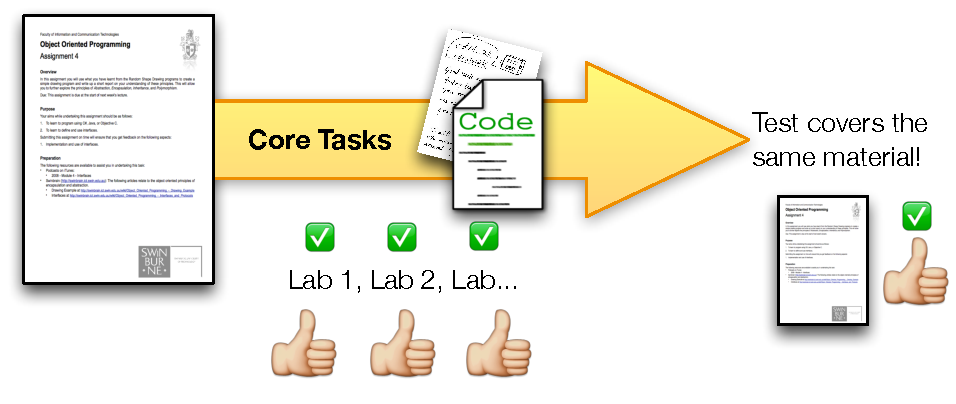
\includegraphics[width=\textwidth]{Tests}
	\caption{Tests cover aspects already presented in the tests, helping verify students completed the work themselves.}
	\label{fig:tests}
\end{figure}

As the tests only assess core competencies, the tests are marked to an exacting standard. Students can be awarded one of three grades: pass, fix or redo. 
\begin{itemize}[noitemsep,nolistsep]
	\item The \emph{pass} grade requires the large majority of the test to be correct. Small issues like minor syntax errors, or other small mistakes can be overlooked, but as a majority the work must demonstrate good mastery of the topics covered. 
	\item \emph{Fix} grades indicate some larger issues are present, but nothing critical and the work still demonstrates a sufficient mastery of the content.
	\item Where the test indicates larger issues that represent critical misunderstandings for the student, their test is marked as \emph{redo} and they must resit the test to be eligible to pass the unit. When no additional test opportunities are available this grade would indicate a \emph{Fail} result for the unit.
\end{itemize}
With both pass and fix grades, students are expected to correct all issues in their test and include the corrected versions in their portfolios. 

It is important to note that the \emph{redo} grade is awarded where critical misunderstandings are demonstrated. This is not equivalent to getting less than 50\%, or some other arbitrary percentage, of available marks. The work is assessed qualitatively, with teaching staff making expert judgements about the level of understanding being demonstrated. The response to even a single question could demonstrate critical misunderstandings, though typically this knowledge would be tested across a number of questions.

Students must include the tests in their portfolios, and the last test has to be passed in examination conditions. All tests also perform a formative role, with students needing to correct any issues themselves and resubmit the work, with the test only being signed off when students have been able to address it to the required standard.

Through a combination of weekly formative feedback, hurdle tests and interviews for higher grades, the model addresses issues of plagiarism without unduly emphasising a punitive approach. This is in keeping with \pref{itm:theory_y} from \cref{cha:guiding_principles}.

% subsection addressing_plagiarism (end)

\section{Summary} % (fold)
\label{sec:ca_summary}


%
% Overall very good - as noted, need to better link the "principles" in Ch4 to Ch3 ones?
% And perhaps rename /number these as  "guidelines"  that can refer back to in Ch 5???
%

This chapter has outlined an overall strategy for teaching introductory programming with portfolio assessment based on an objects-later approach. Using the principles from \cref{cha:guiding_principles}, a model for the development of constructively aligned units was presented. \cref{cha:example_impl} continues this work by demonstrating the application of this model in the creation and delivery of two introductory programming units.

% section summary (end)

% chapter approaching_constructive_alignment_with_portfolio_assessment (end)
%!TEX root = Constructive Alignment for Introductory Programming.tex

\chapter{Constructively Aligned Introductory Programming Curriculum} % (fold)
\label{cha:example_impl}

\graphicspath{{Figures/CAIntroProg/}}

\cref{cha:approach} proposed an approach to delivering constructively aligned introductory programming unit based upon the principles from \cref{cha:guiding_principles}. The proposed apporach makes uses portfolio assessment, with an objects-later apporach that divides the programming content across two introductory programming units. This chapter provides an example implementation of this approach, demonstrating how the principles from \cref{cha:guiding_principles} and the approach from \cref{cha:approach} can be realised in a programming curriculum.

Sections of this chapter relate to the two introductory programming units: introductory programming, and object oriented programming. For each of these units the subsections are ordered to follow the processes from \cref{cha:approach}. First we outline the design of the intended learning outcomes, and the construction of the assessment criteria. This is followed by examples of the various teaching and learning activities and resources developed in implementing this curriculum.  


\section{Introductory Programming} % (fold)
\label{sec:introductory_programming}

\subsection{Aims for Introductory Programming} % (fold)
\label{ssub:intro:aims}

The aim of Introductory Programming is to introduce students to programming and software development fundamentals. While focusing on developing depth in this area, the wholistic nature of the portfolio assessment approach means that programming is placed in the context of software development in general. As a result, this unit will touch on a number of areas.


% subsubsection aims (end)

\subsection{Defining Intended Learning Outcomes} % (fold)
\label{sec:intro:intended_learning_outcomes}

\subsubsection{Influencing Factors} % (fold)
\label{ssub:influencing_factors}

\begin{figure}[htbp]
	\centering
	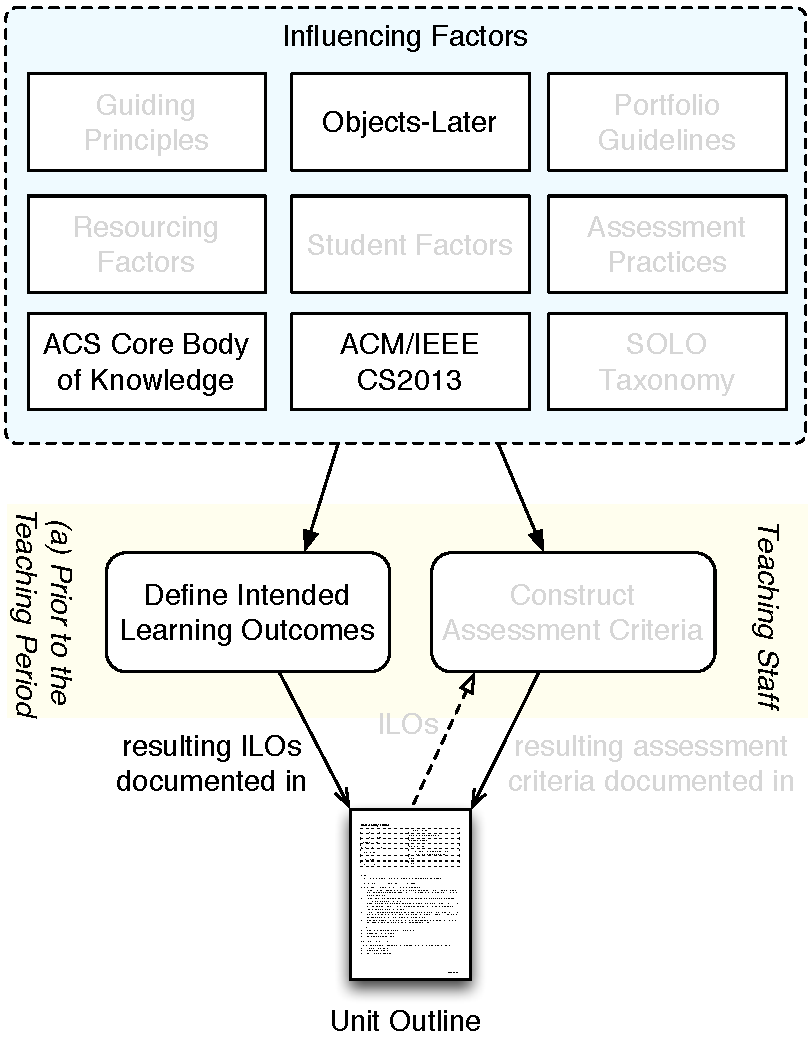
\includegraphics[width=0.7\textwidth]{ILOFactors}
	\caption{Factors that influence the defining of a unit's intended learning outcomes, and the construction of assessment criteria. \fref{fig:defining_ilos}}
	\label{fig:defining_ilos_intro}
\end{figure}

The Association for Computing Machinery and IEEE Computer Society 2013 Computer Science Curriculum \cite{CSC2013} outlines a number of areas to be covered in a Computer Science curriculum. In terms of this model curriculum, the Introductory Programming Unit presented here touched upon a range of areas, as shown in the following list. The primary focus was on the Software Development Fundamentals, but also integrated a number of other areas.

\begin{itemize}[noitemsep,nolistsep]
	\item AL/Algorithmic Strategies: students were introduced to divide-and-conquer, and the idea of recursive backtracking.
	\item AL/Fundamental Data Structures and Algorithms: all students programmed simple numeric algorithms, sequential search, and basic sorting.
	\item CN/Processing: fundamental programming concepts were covered in depth, including algorithms,  implementing algorithms in code, and processes in the software development lifecycle.
	\item DS/Basic Logic: students used truth tables to learn to evaluate boolean expressions.
	\item GV/Fundamental Concepts: applications of computer graphics, double buffering and animation were covered to make programming more interactive.
	\item GV/Geometric Modelling: Optional tasks allowed students to explore procedurally generated models (fractals).
	\item HCI/Programming Interactive Systems: students developed code to manage events and user interactions.
	\item PL/Basic Type Systems: students explored the use of a range of basic types, along with the definition of custom enumerated and record types.
	\item PL/Language Translation and Execution: students are introduced to the topics of compilers and interpreters, as well as run-time layout of memory (call-stack, heap, static data), and manual memory management.
	\item SDF/Algorithms and Design: students were introduced to the concept of algorithms, problem solving using divide-and-conquer, abstraction and program decomposition.
	\item SDF/Fundamental Programming Concepts: students used programming language syntax, develop programs that contained statements, expressions, use variables, simple input and output operations, with conditional control flow, included functions, various parameter passing techniques, and were introduced to the concept of recursion.
	\item SDF/Fundamental Data Structures: programs students implemented made use of arrays, record structures, strings and basic string processing, and students implemented a simple linked list.
	\item SDF/Development Methods: program comprehension was central to the unit, with basic details of program correctness being introduced. Students were also required to use basic refactoring techniques to restructure code, and program tracing was covered as a debugging technique.
	\item SE/Software Processes: students used an iterative software development process model, and were introduced to the phases of the software development lifecycle. 
	\item SE/Software Design: students were introduced to the principles of the structured design paradigm, and used these principles in the design and development of the programs they created.
	\item SE/Software Construction: coding standards, and defensive coding practices were introduced to students.
	\item SP/Professional Ethics: students develop skills in professional practice including self assessment, reflective practice, computer fluency, and general approach to life-long learning.
	\item SP/Professional Communication: to demonstrate their understanding students were required to read, understand and communicate technical material using clear language and visual mediums.
\end{itemize}

The Australian Computer Society (ACS) documented the ICT profession and associated body of knowledge \cite{Gregor:2008}, which indicated graduates should develop both skills and knowledge as part of their undergraduate education. The knowledge area is divided into three aspects: a core body of knowledge, role specific knowledge and complementary knowledge. The introductory programming unit develops student's skills and knowledge.

The skills component of the ACS document drew upon the skills documented in the Skills Framework for the Information Age (SFIA). In terms of the SFIA \cite{SFIA:2011} the Introductory Programming unit aimed to contribute to the development of programming and software development skills to a Level 2, \emph{assist}, standard. This indicates that students need to demonstrate the ability to design, code, test, correct, and document simple programs, and indicates that students are able to assist with the development of larger software solutions.

The ACS divides the core body of knowledge into six areas: problem solving, professional knowledge, technology building, technology resources, service management and outcomes management.

% subsubsection influencing_factors (end)

\subsubsection{Intended Learning Outcomes} % (fold)
\label{ssub:intended_learning_outcomes}

% subsubsection intended_learning_outcomes (end)

Introductory Programming used a procedures-first approach, and focused on the structured programming principles of organising code using \emph{sequence}, \emph{selection} and \emph{repetition}. Students learnt to use functional and modular decomposition to break problems down, and implement solutions using functions and procedures. Data was managed using arrays and custom data types. Pointers and memory management were introduced. Various forms of parameter passing were covered, including pass-by-value and pass-by-reference. Weaved through this was an iterative development process, a focus on writing clear and legible code, and other good programming practices. In addition to writing code, students learnt to read code for the debugging purposes, and to demonstrate their ability to interpret other peoples code. All of this is captured in the intended learning outcomes for Introductory Programming:
\begin{enumerate}[noitemsep,nolistsep]
	\item Apply code reading and debugging techniques to analyse, interpret, and describe the purpose of program code, and locate within this code errors in syntax, logic, and/or good practice.
	\item Describe the principles of structured programming, relate these to the syntactical elements of the programming language used, and the way programs are developed using this language.
	\item Construct small programs, using the programming languages covered that include the use of arrays, functions and procedures, parameter passing with call by value and call by reference, custom data types, and pointers.
	\item Use modular and functional decomposition to break problems down functionally, represent the resulting structures diagrammatically, and implement the structure in code as functions and procedures.
\end{enumerate}

% section introductory_programming (end)






\subsection{Object Oriented Programming} % (fold)
\label{sub:object_oriented_programming}

% subsection object_oriented_programming (end)

Object Oriented Programming takes students who have completed Introductory Programming and introduces them to the object oriented programming paradigm. Students will learn about the core principles of object oriented programming, and how these can be used to create object oriented programs. They will develop programs using integrated development environments, including  unit testing tools. Students will be introduced to visual ways of communicating object oriented designs using the Unified Modelling Language \cite{Fowler:2004}, including both class diagrams and sequence diagrams. Design patterns and heuristics will be used to provide students with a means of evaluating the quality of their designs. As with Introductory Programming students will use a iterative development process. The intended learning outcomes for Object Oriented Programming are:
\begin{enumerate}
	\item Explain the principles of the object oriented programming paradigm specifically including abstraction, encapsulation, inheritance and polymorphism, and explain how these principles are used to create object oriented programs.
	\item Design, develop, test, and debug object oriented programs, using an integrated development environment.
	\item Select and use appropriate collection classes, from the language's class library, to manage collections of multiple objects.
	\item Construct appropriate diagrams and textual descriptions to communicate the static structure and dynamic behaviour of an object oriented solution.
	\item Apply accepted good practices related to the construction of object oriented programs.
\end{enumerate}
% subsection intended_learning_outcomes (end)


Pascal \cite{Becker:2002}



% section concepts_in_introductory_programming (end)

\section{A Simplified Taxonomy to Frame Programming Concepts} % (fold)
\label{sec:a_simplified_taxonomy_to_frame_programming_concepts}

% section a_simplified_taxonomy_to_frame_programming_concepts (end)

\section{Introductory Programming, Procedures First} % (fold)
\label{sec:introductory_programming_procedures_first}

% section introductory_programming_procedures_first (end)

\section{Using Multiple Languages to Focus on Concepts} % (fold)
\label{sec:using_multiple_languages_to_focus_on_concepts}

% section using_multiple_languages_to_focus_on_concepts (end)

% chapter constructively_aligned_introductory_programming_curriculum (end)
%!TEX root = Constructive Alignment for Introductory Programming.tex

\chapter{Supporting the Curriculum with Tools and Technologies} % (fold)
\label{cha:supporting}

\graphicspath{{Figures/Supporting/}}

\section{Visualising Progress to Support Formative Feedback} % (fold)
\label{sec:doubtfire}

\subsection{Background} % (fold)
\label{sub:doubtfire_background}

Formative feedback, \pref{itm:formative}, plays an important role in shaping the teaching and learning environment for the units implemented using the model presented in \cref{cha:approach}. This change helps support the focus on students active construction of their own knowledge, \pref{itm:construct}, but provides an additional challenge as students no longer have marks to guide their behaviour. To help address this challenge, an online task tracking system, named ``Doubtfire'', was developed. 

Doubtfire allowed each student to track their progress against the weekly assessment tasks using a ``burn down chart'' as shown in \fref{fig:example_chart}, a technique adapted from the Scrum agile software development process \cite{Schwaber:2002}. The charts show the cumulative amount of work remaining week by week, which decreases as work is complete, or burns down over time.

\begin{figure}[thb]
  \centering
  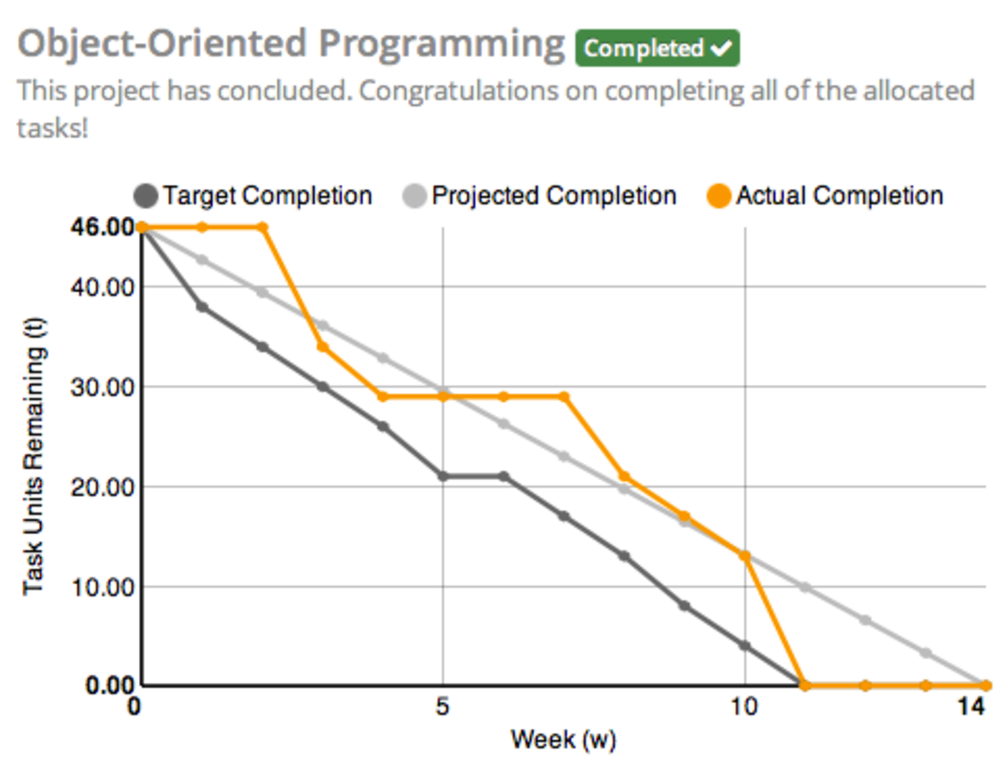
\includegraphics[width=0.9\textwidth]{ExampleChart}
  \caption{An example burn down chart showing progress against weekly tasks.}
  \label{fig:example_chart}
\end{figure}


Agile software development methods \cite{Beck:2001} embrace change \cite{Beck:2000} by allowing for adaptive, periodic adjustment of activities. The basis for this adaptation in Scrum is \emph{empirical} information; a consistent measure of the work remaining (``backlog''), and a measure of the rate work is being completed by the team (``velocity'').

The purpose of a Scrum ``burn down chart'' is to allow stakeholders to consider, in an empirical manner, the velocity of the team with respect to the current backlog. This chart acts as a ``information radiator'' \cite{Cockburn:2002} for the team, providing details on either release or ``Sprint'' iteration schedules. Since quality of work should not be compromised, the requirements (backlog) of work can be adjusted in order to meet the required schedule and cost~\cite{Sutherland:2007}.

In adapting burn down charts as a tool for supporting students engagement with formative assessment tasks, the assessment tasks become the ``backlog''. Students are then able to see the number of tasks remaining, and use their current ``velocity'' to determine if their progress is sufficient to complete the unit on time.

% subsection background (end)

\subsection{Requirements} % (fold)
\label{sub:doubtfire_requirements}

The central requirement for the Doubtfire tool was to provide students with visual feedback on their progress using burn down charts. The burn down charts provide students with a visual representation of the tasks they need to complete over the teaching period, and show the number of tasks, their scheduled due date, and estimated task effort. Students should be able to use the tool to assess their progress throughout the teaching period, and to determine whether they need to increase their rate of progress (velocity) and, if so, commit more time to the unit or take greater advantage of resources available to them. 

It was also seen that the scrum-style marking of tasks as completed could be extended to allow students to indicate if they were working on, or having trouble with, particular tasks. This requirement aimed to increase student engagement with the tool, and improve likelihood that they would make active use of it throughout the teaching period.

To account for task heterogeneity, staff needed to be able to set a specific \emph{weight} for each task. This weight represents the estimated effort students needed to expend to satisfactorily complete the task. Rather than specifying task weight in terms of hours, this was done in a more abstract unit. One popular approach with agile software development projects is to assign tasks ``\emph{t-shirt size}'' weights \cite{Peixoto:2010}. Using this approach tasks have their weight set to a common t-shirt size: \emph{extra small}, \emph{small}, \emph{medium}, \emph{large}, \emph{extra large} etcetera. The t-shirt sizes are then allocated weights, with each increment in size doubling the associated weight: extra small had a weight of one, small a weight of two, medium four, etcetera.

Task weights needed to be incorporated into the burn down chart, with each chart showing the cumulative number of \emph{task-points} remaining. Using task-points in the burn down charts enables the chart to visually show weeks where more, or less, effort is likely to be required.

Progress also needed to be projected to indicate an expected completion date. This projection can be calculated from the average number of task-points the student completes each week.  For example, if six task-points were completed in one week, based on the velocity, a thirty-six task-point project is expected to be completed in six weeks. Each student's projected completion should be recalculated as tasks and weeks progress. 

As an interactive system, Doubtfire had a number of requirements to ensure that it could be best utilised by all targeted users. The following requirements were identified:
\begin{itemize}[noitemsep,nolistsep]
  \item \textbf{Online}: students needed to be able to easily access the tool both in and out of scheduled class times. It was decided to make Doubtfire an online tool, thereby making it accessible from virtually anywhere. It also simplifies the development progress with only web platforms needing to be supported, and avoids the need for students to install client software.
  \item \textbf{Easy to use}: the tool need to be simple enough to use, so the usability of the tools must provide as small a barrier as possible to student adoption.
  \item \textbf{Mobile friendly}: students should be able to quickly check, and update, their progress from a range of devices. Ensuring that Doubtfire can be easily accessed via a mobile device will encourage students to access the tool even when they are away from their computers. 
  \item \textbf{Aesthetically pleasing user interface}: to encourage adoption of the tool among students, a visually appealing user interface is ideal.
\end{itemize}
Simply, our aim was to create a tool that was simple and appealing for students to use and was easily accessible from a range of devices and locations. Students not should feel that interaction with the tool is work.

In addition to students, Doubtfire also addressed needs of teaching staff. Tutors were responsible for managing classes, and therefore needed to be able to respond to student actions in the tool. Convenors had overall responsibility for the unit, and needed to be able to observe the performance of the student cohort and perform simple administrative actions. All teaching staff benefited from the requirements already listed. Most importantly, the mobile nature allowed tutors to easily check and update students' progress during scheduled classes.

\medskip

In terms of the development and deployment of the tool, a number of software qualities are desirable. These include:
\begin{itemize}[noitemsep,nolistsep]
  \item \textbf{Supports the teaching environment}: the tool plays a supportive role, and should therefore fit inside the teaching environment; it should not be necessary to fit the teaching environment around the tool.
  \item \textbf{Quick to develop and extend}: it should be easy to produce features and adapt the tool to ensure it remains relevant to the students.
  \item \textbf{Controllable}: the schema that defines the way tutors and students interact over tasks must be easy to alter to allow for adaptation if assessment criteria change.
\end{itemize}

% It is valuable to add features that track student behaviour in the tool to:
% \begin{itemize}[noitemsep,nolistsep]
%   \item Determine whether the expected use of the software matches the actual.
%   \item Identify possible issues in the unit curriculum, such as inconsistent assignment weighting.
%   \item Identify possible flaws in the rule system governing student and tutor interaction in the software.
%   \item Exploit the information to insights into general teaching issues.
%   \item Optimise the experience based on how students use the software.
% \end{itemize}
% As this information is constantly generated through use of the tool, it is simply a matter of storing what actions have been performed. This provides unambiguous information that can then be analysed through quantitative methods.

% This section has described the requirements we deemed non-negotiable in the production of an effective progress management tool for the users identified. There are a number of minor requirements that were not considered significant enough to describe here. From these requirements were produced a number of features accessible to the convenor, tutor and student user groups, which are discussed in the following section.

% subsection requirements (end)

\subsection{Doubtfire Solution} % (fold)
\label{sub:doubtfire_solution}

\subsubsection{User Roles} % (fold)
\label{sub:user_roles}

The three user groups in Doubtfire were Convenor, Tutor and Student. Each of these groups had access to a different set of features as described in \tref{tab:user_features}. Convenor and Tutor roles were provided to support teaching staff, with the students having a separate role. 

% This is what can do with the tool
\begin{table}[htbp]
  \renewcommand{\arraystretch}{1.6}
  \centering
  \caption{Available features for each user group in Doubtfire}
  \label{tab:user_features}
  \begin{tabular}{c|p{0.9\textwidth}}
    Role & \multicolumn{1}{c}{Features} \\ \hline\hline
    \multirow{5}{*}{\begin{sideways}\parbox{14mm}{Convenor}\end{sideways}}
    & - \textbf{Unit Administration}: including the ability to enrol students and create tasks. \\
    & - \textbf{Monitor Student Progress}: view distribution of students by progress indicators. \\
    & - \textbf{Monitor Task Progress}: view progress distribution for each of the unit's tasks. \\
    & - \textbf{Examine Student Progress}: view the list of tasks and their associated status by student. \\
    & - \textbf{Update Task Status}: mark student work as complete. \\ 
    & \\
    \hline\hline
    \multirow{2}{*}{\begin{sideways}\parbox{10mm}{Tutor}\end{sideways}}
    & - \textbf{Examine Student Progress}: view the list of tasks and their associated status by student. \\
    & - \textbf{Update Task Status}: mark student work as complete. \\ 
    & \\
    \hline\hline
    \multirow{3}{*}{\begin{sideways}\parbox{11mm}{Student}\end{sideways}}
    & - \textbf{Update Task Status}: mark student work as complete. \\ 
    & - \textbf{Monitor Progress}: view progress on task completion using a burn down chart showing Target, Actual and Projected completion. \\
    & \\
  \end{tabular}
\end{table}

Unit convenors are responsible for the overall delivery and management of the unit. To support this role, Doubtfire provided these users with the tools to set up unit tasks and enrol students. A dashboard provided Convenors with an overview of student progress, and enabled quick access to views of student progress by task, and to individual students via their scheduled class. \fref{fig:dashboard} shows an example overview of students progress for a single unit from the Convenor Dashboard. While, \fref{fig:task_chart_view} shows an example chart that visualises the distribution of student status for each task. In addition to these tasks, Convenors also had the ability to perform the same actions as Tutors.

\begin{figure}[thbp]
  \centering
  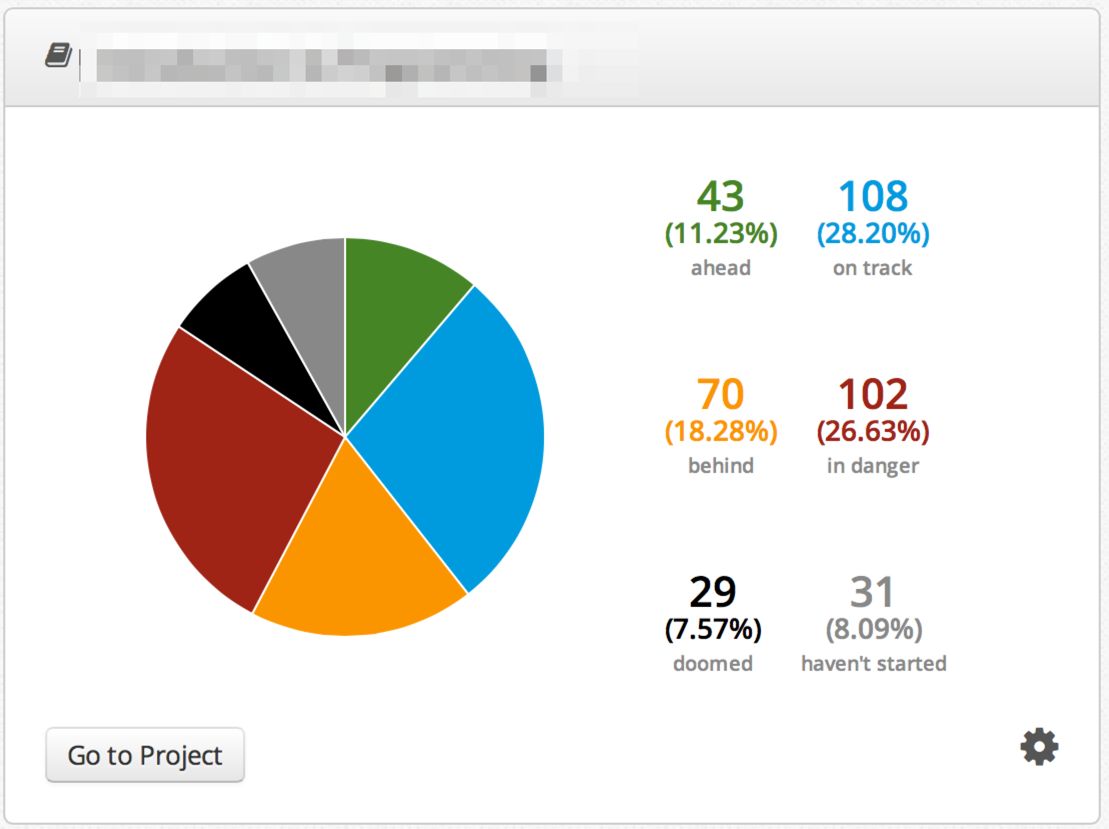
\includegraphics[width=0.8\textwidth]{Dashboard}%
  \caption{Overview of progress by unit from the Convenor Dashboard.}%
  \label{fig:dashboard}%
\end{figure}

\begin{figure}[thbp]
  \centering
  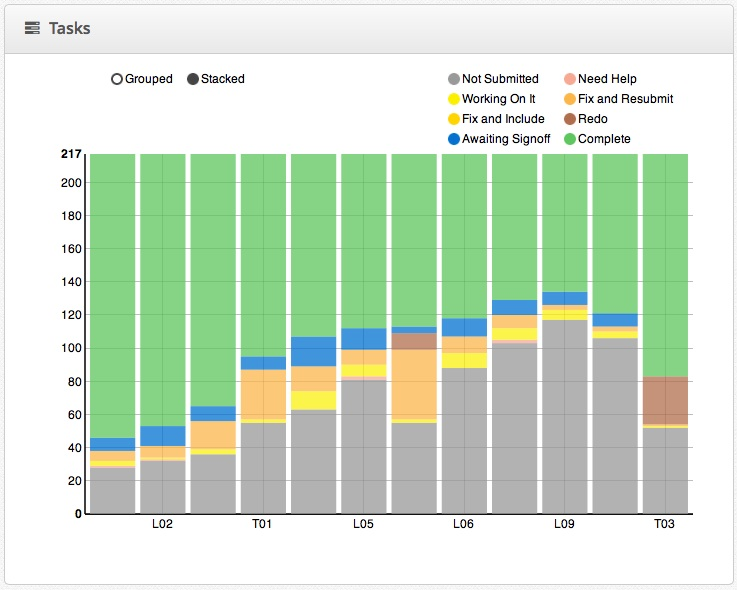
\includegraphics[width=0.8\textwidth]{TaskChart}%
  \caption{Convenor view showing distribution of student status by task}%
  \label{fig:task_chart_view}%
\end{figure}

Tutors are responsible for conducting the tutorial classes, and providing formative feedback for the students in these classes. To support this role, Doubtfire provided tutors with a class list view showing student progress. From the class list, tutors could drill down to view individual students and their burn down charts, and provided a convenient means of updating task status. 

\fref{fig:tutor_view} shows an example of the class list used by Tutors. The class list shows the students in the tutors class, their names and id numbers have been obscured in \fref{fig:tutor_view}, with each task being represented by a coloured rectangle indicating the current status of the task for that student. Tutors are able to update the status of a student's tasks directly from the class list.

\begin{figure*}[thbp]
  \centering
  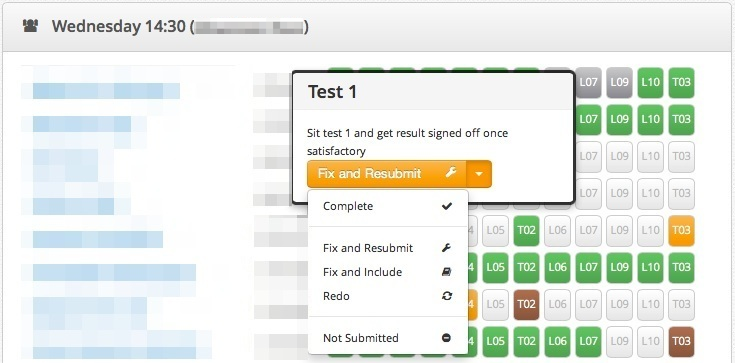
\includegraphics[width=0.8\textwidth]{TutorView}
  \caption{Tutors viewed class groups and could adjust task states}
  \label{fig:tutor_view}
\end{figure*}

\fref{fig:home_page} shows an example of the dashboard provided to students. Each student was provided with a dashboard showing their progress for the units they were enrolled in. Students could view their burn down chart and task statuses by selecting units from their dashboard. When viewing a unit, students could update the status of their tasks as shown in \fref{fig:task_list}.

\begin{figure*}[thbp]
  \centering
  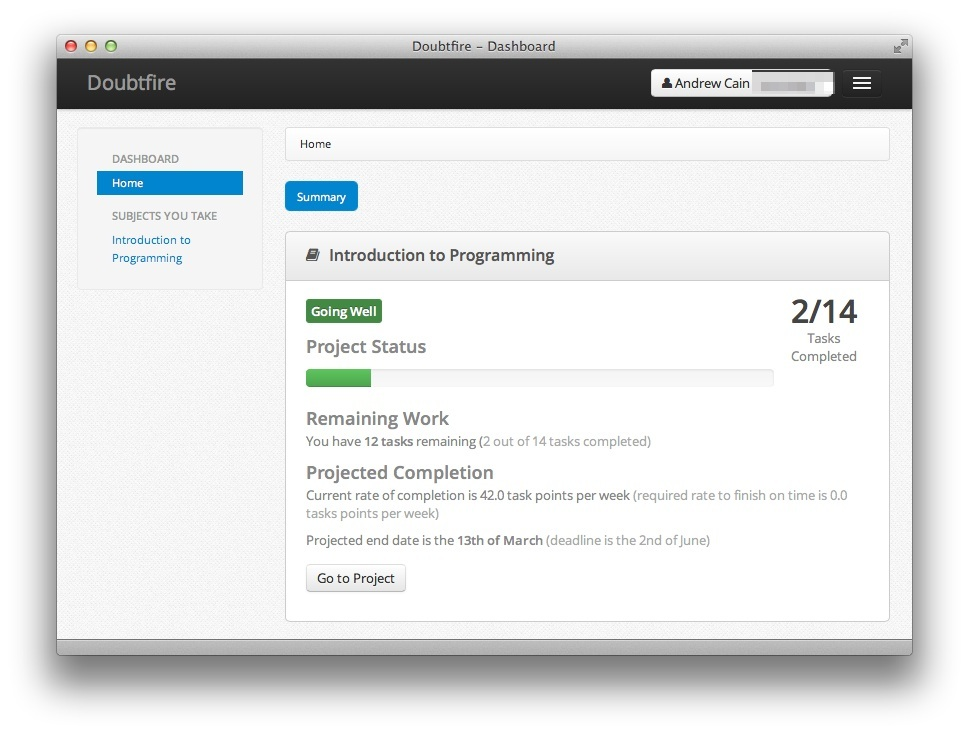
\includegraphics[width=0.8\textwidth]{HomePage}%
  \caption{Student home page in Doubtfire, showing progress on all enrolled projects}%
  \label{fig:home_page}
\end{figure*}

\begin{figure}[thbp]
  \centering
  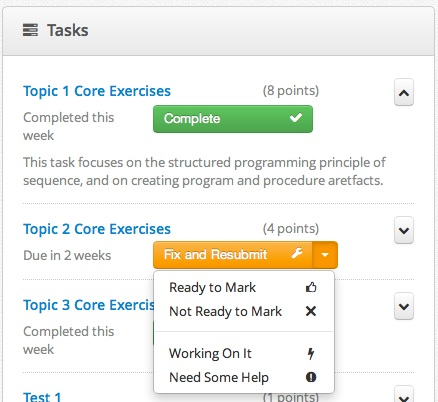
\includegraphics[width=0.6\textwidth]{StudentTasks}
  \caption{The Tasks list enabled students to view and change task status}
  \label{fig:task_list}
\end{figure}

Student progress could be viewed as a burn down chart that consisted of three lines, as shown in \fref{fig:example_chart}. The lines indicated:
\begin{itemize}[noitemsep,nolistsep]
  \item \textbf{Actual Completion}: showed the number of task-points signed off for the student by week.
  \item \textbf{Target Completion}: showed the recommended schedule from the task due dates set by the convenor.
  \item \textbf{Projected Completion}: indicated the current velocity, which was then projected to indicate an expected end date if current velocity was maintained.
\end{itemize}

% subsection user_roles (end)

\subsubsection{Task Processes} % (fold)
\label{sub:task_processes}

Tasks in the Doubtfire system could have one of a number of statuses, with different users being responsible for updating task statuses at various times during unit delivery. The main statuses and the transitions between these is shown in \fref{fig:basic_process_chart} as a UML State Chart. 

\begin{figure}[thbp]
  \centering
  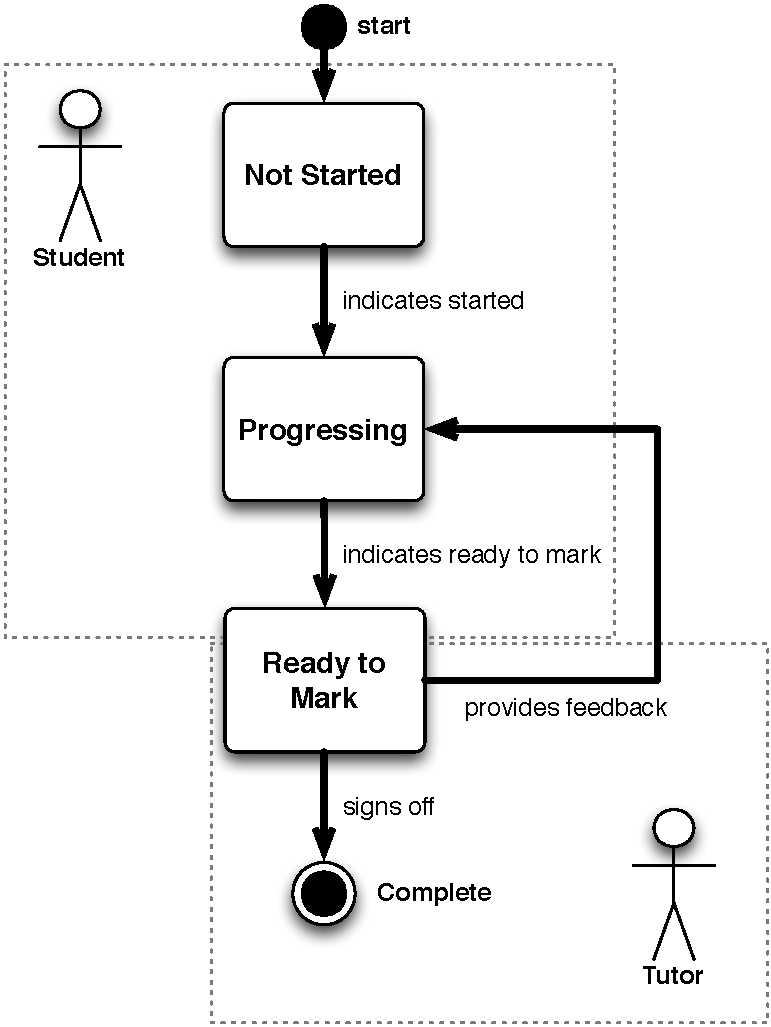
\includegraphics[width=0.7\textwidth]{BasicProcessStateChart}
  \caption{UML state chart showing task states and transitions.}
  \label{fig:basic_process_chart}
\end{figure}

Initially all tasks are set to the \emph{Not Started} status. When students begin work on the task they are encouraged to update its status to \emph{Progressing}, and when it is ready for assessment to the \emph{Ready to Mark} status. Once tutors receive the work, they examine the work and provide the student with formative feedback. After having discussed the task with the student, the tutor updates the status by either returning it to a \emph{Progressing} status if the task needs to be fixed, or signing the task off as \emph{Complete}.

The \emph{Progressing} status was divided into a number of sub-states for the purpose of providing students with finer-grained feedback. 

Students were able to set the status of a task to \emph{Working on It} or \emph{Needs Help} to indicate their current progress on the task to their tutor and to the unit convenor. \emph{Fix} and \emph{Redo} statuses could be used by students to indicate that tasks needed some aspects adjusted (the \emph{Fix} status) or that it should be redone (the \emph{Redo} status). These status, shown in \fref{fig:detailed_states}, were designed to help provide more accurate details of progress for both staff and students. Students indicated how they were progressing with the tasks, and staff could provide feedback on the outcomes students had achieved.

\begin{figure}[thbp]
  \centering
  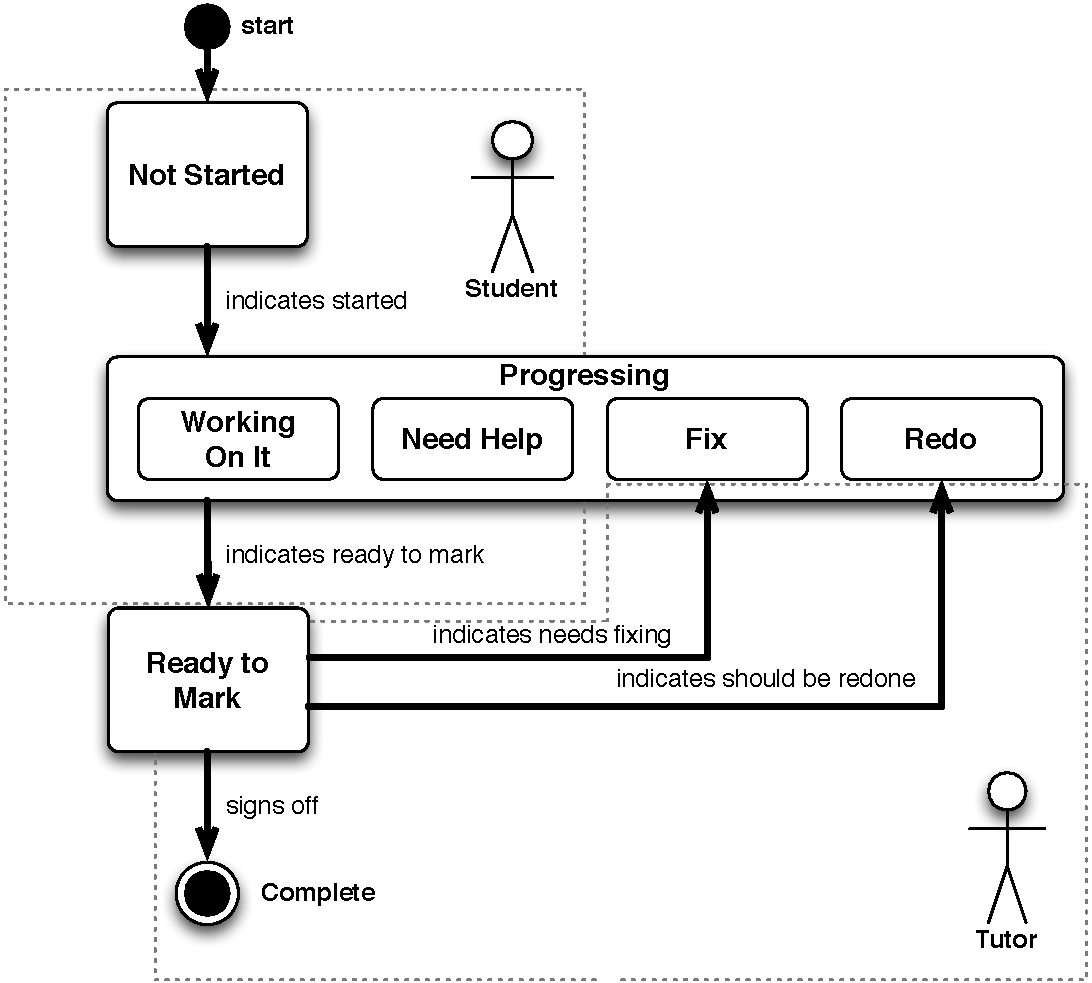
\includegraphics[width=\textwidth]{DetailedStepsInProgress}
  \caption{UML state chart showing the detailed states within the Progressing superstate.}
  \label{fig:detailed_states}
\end{figure}

% subsection doubtfire_solution (end)

\subsection{Use of Doubtfire} % (fold)
\label{sub:use_of_doubtfire}

While \cref{cha:evaluation} provides a more in-depth discussion of the use of Doubtfire, this section will briefly comment on how it was used in the delivery of both the introductory programming and object oriented programming units. In both cases the teaching and learning activities from \cref{cha:example_impl} were used as the tasks to be completed, and teaching staff assigned each a weighting to represent its relative size.

The effectiveness of the tool, for students, depended on their engagement with the unit. The more capable students made active use of Doubtfire, and responded quickly to addressing issues and closing gaps in their knowledge. Students who struggled to complete the weekly tasks generally made poor use of the tool at the start of the teaching period, but engaged actively later in the semester. While some, more disengaged, students avoided use of the system and attempted to establish progress on their own terms. 

For teaching staff, the Doubtfire tool provided useful information on how students were engaging with the formative process. It was easy to see which students were doing well, to identify those who were falling behind, and those who were not engaging with the unit at all. This information was used to prompt students, encouraging those who were doing well and suggesting appropriate resources for those who were falling behind.

\subsection{Summary} % (fold)
\label{sub:doubtfire_summary}

The strong use of formative feedback in the model provides a challenge as students cannot be motivated by marks during the teaching period. This could lead to students allocating insufficient time to complete the unit's tasks, allowing them to fall behind in the unit.

Doubtfire helped to address this concern through the use of burn down charts that visually represented the amount of work students had remaining in the unit. By using this tool staff and students were able to monitor progress throughout the teaching period.

% subsection summary (end)

% section doubtfire_using_burndown_charts_to_support_formative_feedback (end)

\section{Resources to Support Concept Focus} % (fold)
\label{sec:arcana}

\subsection{Background} % (fold)
\label{sub:arcana_background}

Concepts were central to \emph{what} we aimed to teach. \pref{itm:concepts} indicates that we should aim to focus on concepts over language syntax. In addressing this principle the introductory programming unit from \cref{cha:example_impl} had little, if any, coverage of syntax in the lectures, leaving these details instead to teaching and learning resources.

While concepts are important, syntax details need to be available to help students turn these concepts into working code. In order to achieve this two resources were made available: the ``Programming Arcana'' \cite{Cain:2013arcana}, and a range of video podcasts via iTunesU. Each of these resources was designed to support the concept focus and to provide details on the language syntaxes used in the unit. These resources used a range of audible, visual and textual mediums to present the details so as to better support a range of learning approaches.

% subsection background (end)

\subsection{Programming Arcana} % (fold)
\label{sub:programming_arcana}

One of the central ideas of ``Beyond Bullet Points'' is to fully document the notes attached to a presentation's slides \cite{Atkinson:2007}. In effect, the details are moved from the slide itself to the slides' notes, which can then be printed as an informative handout. In our approach this worked against \pref{itm:agile}, and would have resulted in significant effort being expended on the creation of each week's presentation, thereby adding resistance to changing these if they were found to be ineffective.Instead of documenting these notes in the presentations themselves, they were written up in a separate resource: the \emph{Programming Arcana} \cite{Cain:2013arcana}.

Documenting the language details in a separate text also helped to address another issue raised as a result of choosing Pascal as one of the programming languages. Pascal is not currently a popular language with text book writers, and while the Free Pascal Language Reference Guide \cite{FPC:2013lang} provides details of the language it is not designed for beginners.


\subsubsection{Chapter Sequence} % (fold)
\label{ssub:chapter_sequence}

Chapters in the Programming Arcana were designed to align with the main concept topics from the introductory programming unit. This meant that the text needed to embody the concepts-first approach, \pref{itm:concepts} discussed in \cref{cha:guiding_principles}. To best support this, each chapter needed to focus on providing a coherent set of concepts that built upon concepts presented earlier in the text. The following list illustrates how the programming concepts are presented in the Programming Arcana. This is followed by a discussion of how well the text was able to embody the concept first approach.

\begin{enumerate}[noitemsep,nolistsep]
  \item \textbf{Building Programs}: introduced students to the tools they required, and showed them a basic program they could compile to check the tools were working. The concepts in this chapter included: 
  \begin{itemize}[noitemsep,nolistsep]
    \item \textbf{Programs} were introduced as a sequence of instructions that get the computer to perform actions.
    \item \textbf{Machine and Assembly code} provided some context as to why compilers are necessary. Machine code was presented as the computers natural language, and Assembly as a first step toward making this code more human-friendly.
    \item \textbf{Source code and compilers} introduced the ideas of third generation languages, and the need for a compiler to convert this code to machine code.
    \item The \textbf{Terminal} was introduced as a means of running programs, and the steps for using the compiler were presented. This section also introduced the \textbf{BASH} shell, along with commands to navigate through the file system. 
    \item The final concept outlined the code for a \textbf{Hello World} program in C and Pascal, together with the steps needed to compile and run this program. 
  \end{itemize}
  \item \textbf{Program Creation}: described how code could be written to create a \emph{Program}.
  \begin{itemize}[noitemsep,nolistsep]
    \item This introduced the idea that a \textbf{Program} could be created in code, and that it had a name and a list of instructions for the computer to perform.
    \item \textbf{Procedures} were introduced as a named group of instructions that performed a task. These instructions could be run using a \textbf{Procedure Call}.
    \item The idea that procedures could be distributed in a \textbf{Library} was introduced.
    \item Programming language terminology was also introduced, include \textbf{Statements} as the technical term for commands, \textbf{Expressions} for calculated values, \textbf{Types} to describe different kinds of data, and \textbf{Identifiers} as the names for artefacts such as the programs created and the procedures called. 
    \item \textbf{Comments} were also discussed as a means of documenting code.
  \end{itemize}
  \item \textbf{Procedure Declaration}: introduced the idea that you can create your own procedures to encapsulate the steps of a task. 
  \begin{itemize}[noitemsep,nolistsep]
     \item \textbf{Procedure declaration} described how procedures could be created as a sequence of instructions that are run when the procedure is called.
     \item The concept of a \textbf{Program} was extended to indicate that a program's code could include procedure declarations.
   \end{itemize} 
  \item \textbf{Storing and Using Data}: made programs more dynamic with variables and constants to store data, and functions to calculate values.
  \begin{itemize}[noitemsep,nolistsep]
    \item \textbf{Variables} were introduced as a means of storing data that changed within the code, while \textbf{Constants} were introduced as a means of storing data that does not change. 
    \item The \textbf{assignment statement} was introduced as the means of storing a value in the variable, and the concept of an \textbf{expression} was updated to indicate it could read the value from the variable.
    \item Programming terminology related to the location of a variable was introduced, with \textbf{local variables} being declared within a procedure, \textbf{global variables} within the program, and \textbf{parameters} as a means of enabling data to be passed to a procedure.
    \item The different parameter passing options were presented, with \textbf{pass-by-value} indicating that the value of the expression in the procedure call was passed, while with \textbf{pass-by-reference} the parameter needs to be passed a \emph{variable} to which it will refer.
    \item Creating \textbf{Functions} to calculate values was also introduced, along with updating expressions to indicate the use of \textbf{function calls}.
    \item To realise these concepts, the previous \textbf{statement}, \textbf{program} and \textbf{procedure declaration} concepts were updated.
  \end{itemize}
  \item \textbf{Control Flow}: introduced the structured programming principles, along with the control flow mechanisms of selection and repetition.
  \begin{itemize}[noitemsep,nolistsep]
    \item \textbf{Boolean data} was discussed as a means of directing the control flow statements. This included the use of \textbf{comparisons} to calculate boolean values, as well as the \textbf{logical operators} (\emph{and}, \emph{or}, and \emph{not}).
    \item Selection was described in terms of \textbf{branching}, this included the ideas of \textbf{if statements} and \textbf{case statements}.
    \item \textbf{Looping} introduced \textbf{pre-test loops} that repeated code zero or more times, and \textbf{post-test loops} that repeated code one or more times. 
    \item Other control flow statements were covered in the section on \textbf{jumping}. This included \textbf{break} to jump out of a loop, \textbf{continue} to jump to the end of a loop, \textbf{exit/return} to jump out of a function or procedure, and \textbf{goto}.
    \item Finally, the idea of grouping statements in a \textbf{compound statement} was presented, and explained in terms of providing a sequence of statements within the control flow statements.
  \end{itemize}
  \item \textbf{Managing Multiple Values}: presented the use of arrays.
  \begin{itemize}[noitemsep,nolistsep]
    \item \textbf{Arrays} were presented as a means of managing a number of values in a single variable. \textbf{String} was discussed as an example of an array students had already been working with.
    \item The importance of \textbf{pass-by-reference} was reintroduced.
    \item \textbf{For loops} were introduced as a convenient means of looping over the elements of an array. 
    \item The \textbf{Assignment statement} and \textbf{Expression} concepts were updated to indicate how arrays could be used.
  \end{itemize}
  \item \textbf{Custom Data Types}: described how developers can create types to help them organise the data in their programs, much as functions and procedures helped to organise functionality.
  \begin{itemize}[noitemsep,nolistsep]
    \item \textbf{Types} were described again, in more detail to provide context. 
    \item \textbf{Type declaration} was discussed along with \textbf{records/structs}, \textbf{enumerated types} and \textbf{unions}. This required an update to the concept of what a \textbf{Program} can contain.
    \item The \textbf{Assignment statement} and \textbf{Expression} concepts were updated to indicate how the various custom types could be used.
  \end{itemize}
  \item \textbf{Dynamic Memory Allocation}: extended programs beyond the confines of the stack, allowing the allocation of data on the heap.
  \begin{itemize}[noitemsep,nolistsep]
    \item The \textbf{Stack} and \textbf{Heap} were discussed. This highlighted the need for values on the stack to have a known size, requiring another ``space'' for allocating data when its size is not known at compile time.
    \item \textbf{Pointers} were introduced as a means of referring to space allocated on the Heap.
    \item The need for specific actions to \textbf{allocate memory}, and to \textbf{free} that allocation were also presented.
    \item Common \textbf{issues with pointers} were also discussed, indicating why they are likely to occur and how to address these issues. This included \textbf{access violations}, \textbf{memory leaks} and \textbf{accessing released memory}. 
  \end{itemize}
  \item \textbf{Input and Output}: described how to save and load data from file.
  \begin{itemize}[noitemsep,nolistsep]
    \item The concept of \textbf{persisting data} discussed the idea of a process and its memory being freed after the program terminates. This lead to details on saving data from the program's memory onto persistent storage.
    \item \textbf{Files} and text and binary \textbf{file formats} were discussed. 
    \item \textbf{Interacting with Files} described the typical input and output operations you are likely to perform on a file.
    \item \textbf{Other output devices} related the concepts presented to terminal input/output and the idea that the same concepts applied to sending data across a network connection.
  \end{itemize}
\end{enumerate}

In proposing \pref{itm:concepts}, with its focus on programming concepts, \cref{cha:guiding_principles} outlined the requirement that we needed to ``Introduce programming concepts incrementally''. The Programming Arcana provides an example of how the details of the programming language can be presented in such a way as to ensure most topics are presented incrementally, with each topic building upon the previously presented topics. 

There were two cases where concepts could not be suitably explained within the overall context presented in a chapter. Other than these two cases, all other chapters were able to explain all concepts in terms of the presented, or previously presented, concepts.
\begin{itemize}[noitemsep,nolistsep]
  \item In Chapter 1, of the Programming Arcana, a program was given to enable students to compile something before they understood what it represented. However, the main focus of the chapter was the tools being presented and not the program's code. 
  \item Chapters 2 and 3 of the Programming Arcana passed values to procedures before topics related to how data can be stored in a program. The idea that data can be passed to a procedure was covered, but not how that data was received.
\end{itemize}

In general, mapping the concepts to syntax was simpler for the Pascal programming language. The main challenges with the C language\footnote{The C code was compiled with a C++ compiler to add support for function and procedure overloading, and pass-by-reference.} were the standard input and output functions, \texttt{printf} and \texttt{scanf} and associated details such as format strings and pointers, and the need to understand arrays before working with strings. This meant that early topics were reduced to using string literals and limiting variables to working with numeric values. In this way the one example could be mapped to both C and Pascal. 

The use of Pascal in the first part of the unit meant that teaching and learning activities could take advantage of Pascal's more convenient support for strings and terminal input and output. For example, consider a program that asked the user to enter their name and then echoes back a welcome message. In C this requires an understanding of variables, format string syntax, arrays, pointers, and how arrays are automatically passed by references where other types are not. In Pascal the same program only requires an understanding of variables and pass-by-reference.

% \begin{itemize}[noitemsep,nolistsep]
%   \item Introduce programming concepts incrementally;
%   \item Provide students with time to put concepts into practice;
%   \item See syntax as a means to an end, not an end in itself;
%   \item Avoid using language features before concepts that can explain their use; and
%   \item Map concepts to code using programming language grammars.
% \end{itemize} 


% subsubsection chapter_sequence (end)

\clearpage
\subsubsection{Chapter Layout} % (fold)
\label{ssub:chapter_layout}

Each chapter of the Programming Arcana had a similar sequence to its sections. This aimed to promote a consistent approach to studying each of the topics. In keeping with \pref{itm:concepts}, the concepts were presented as the focus of each chapter. % The was followed with examples of how to apply the concepts, and then the language syntax for C and Pascal. Following this a section was dedicated to tracing the execution of the concepts in a conceptual machine, akin to the notional machine discussed by \citet{DuBoulay:1986}. Each chapter then concluded with examples and exercises.

\begin{enumerate}[noitemsep,nolistsep]
  \item \textbf{Concepts}: each chapter started with a list of related concepts.
  \item \textbf{Applying the Concepts}: following the concepts was an example of applying those concepts in an abstract sense, using pseudocode and flowcharts to illustrate how the concepts could be applied.
  \item \textbf{Syntax in C and Pascal}: details of how to code the concepts were first presented in C, with the following section detailing the syntax for Pascal.
  \item \textbf{Understanding the Concepts}: traced the execution of the pseudocode on a conceptual machine, with the aim of showing students how the concepts are realised at run time. 
  \item \textbf{Examples}: listed a number of examples, each presented in pseudocode then in C and Pascal code.
  \item \textbf{Exercises}: a sequence of exercises students could use to develop their understanding of the topic.
\end{enumerate}

Details of the sections related to presenting the concepts follow. This outlines how the Programming Arcana implemented the concept-based approach, and reinforce the focus on concepts over syntax throughout the material presented. 

\clearpage
\paragraph{Concepts:} % (fold)
\label{par:concepts}

Each chapter started with a section that provided details of the concepts being presented. This section started with a brief overview that described how all of the concepts are related. This was followed by subsections that covered the details of each concept, with a textual description, visual concept map, and a series of notes with important details related to the topic. At the end of the concept section an overall concept map was included that visually showed the relationship between the concepts covered. 

\fref{fig:arcana_concepts} shows an example of the concept of branching from chapter 5 of the Programming Arcana. The diagrams were deliberately drawn using irregular shapes to indicate these were a conceptualisation, rather than an exact representation of the associated concepts.

One of the design goals was to fit each concept on a single page. This goal aimed to help support students active construction of their knowledge, \pref{itm:construct}. Aiming to keep each topic to a single page ensured that we focused on the most important details, and where topics expanded over multiple pages the details were examined to ensure we had not included any unnecessary details.

\begin{figure}[h]
  \centering
  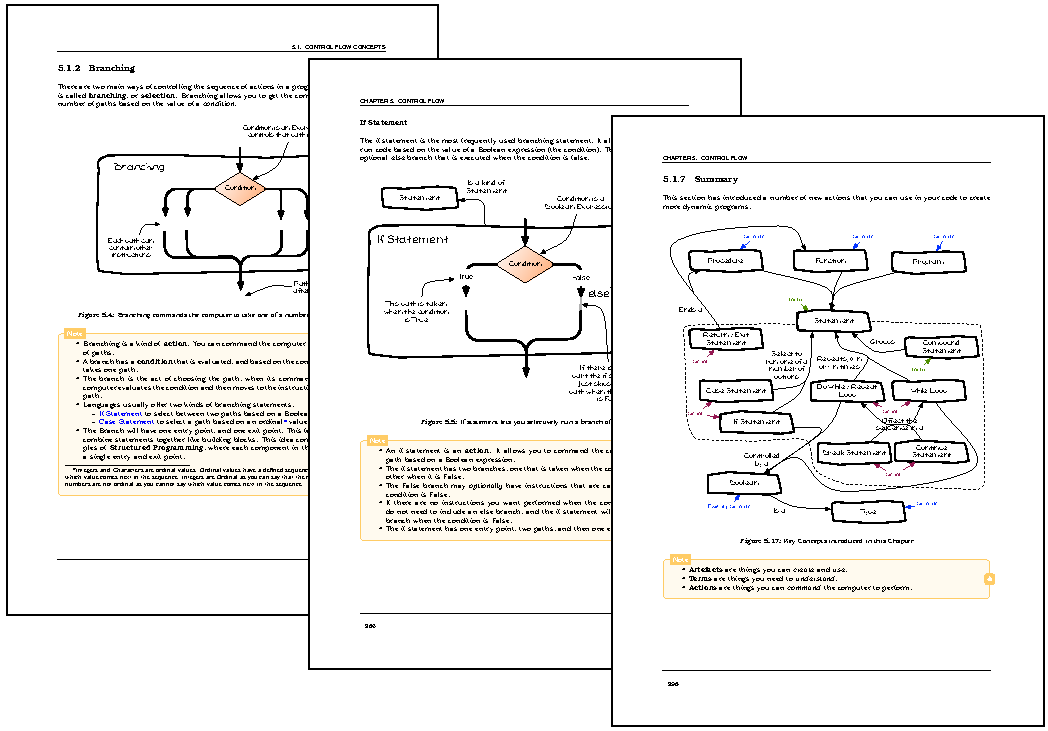
\includegraphics[width=0.7\textwidth]{ArcanaConcepts}
  \caption{Example concept pages from the Programming Arcana.}
  \label{fig:arcana_concepts}
\end{figure}

% paragraph concepts (end)

\clearpage
\paragraph{Applying the Concepts:} % (fold)
\label{par:applying_the_concepts_}

After the concepts were presented, the next section outlined how these concepts could work together to create an example program. This section always started with a specification of a program that was to be created. This was then followed by a discussion of how a the program could be designed using the concepts covered to that point in the text. The description of the design included pseudocode, flow charts, sequence diagrams and structure charts, and the section concluded with a complete design for specified program. \fref{fig:arcana_applying} shows an example of some pages related to applying control flow concepts.

Explanatory text accompanied the design, and highlighted how the concepts covered contributed to the end result. This discussion also presented a way of approaching problems using the concepts to introduce students to the idea of designing their own programs.

\begin{figure}[h]
  \centering
  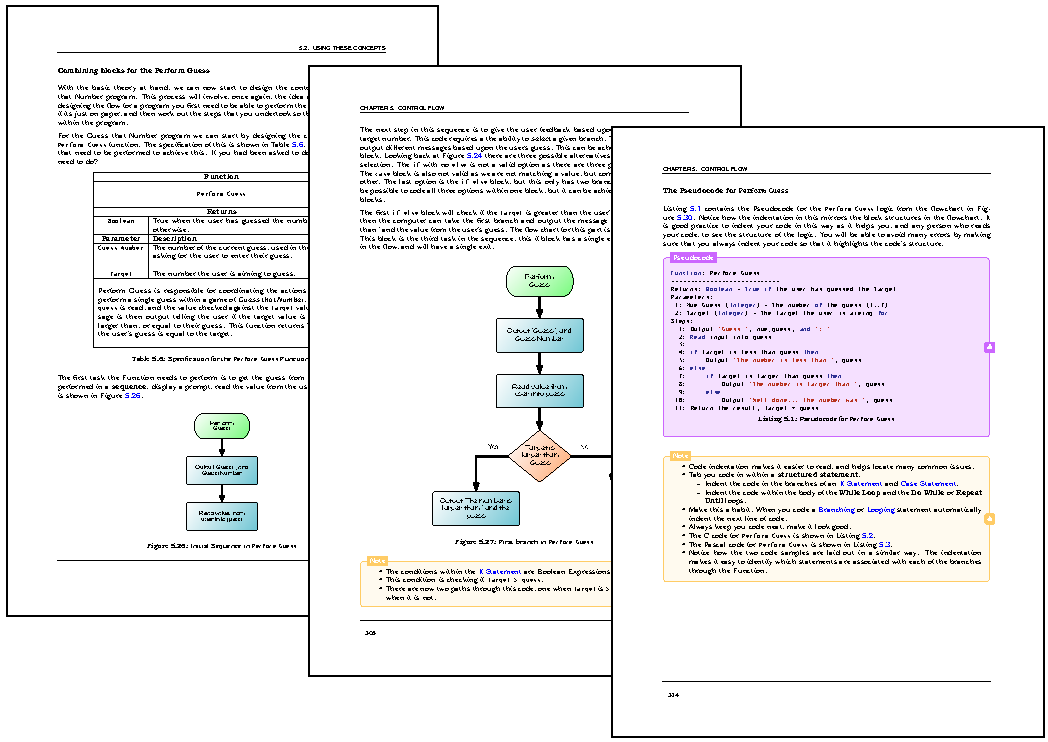
\includegraphics[width=0.7\textwidth]{ArcanaApplying}
  \caption{Example pages related to applying the concepts from the Programming Arcana.}
  \label{fig:arcana_applying}
\end{figure}

% paragraph applying_the_concepts_ (end)

\clearpage
\paragraph{Syntax} % (fold)
\label{par:syntax}

Having covered the concepts, and how they can be used to create a conceptual program, the next two sections dealt with realising these concepts in C and Pascal code. The syntax sections of the Programming Arcana started with an implementation of the program designed in the section on applying the concepts, which was followed by the grammar to implement the various concepts discussed. An example of pages from this section is shown in \fref{fig:arcana_syntax}.

As with the concepts, the aim was to explain each aspect of the syntax in a single page. This page started with a textual description of the syntax, which was followed by a graphical representation of the grammar and then one or two examples of its implementation in code. The grammar and examples presented focused on best representing the concepts, in many cases only presenting a suitable subset of what was possible with the programming language. 

\begin{figure}[h]
  \centering
  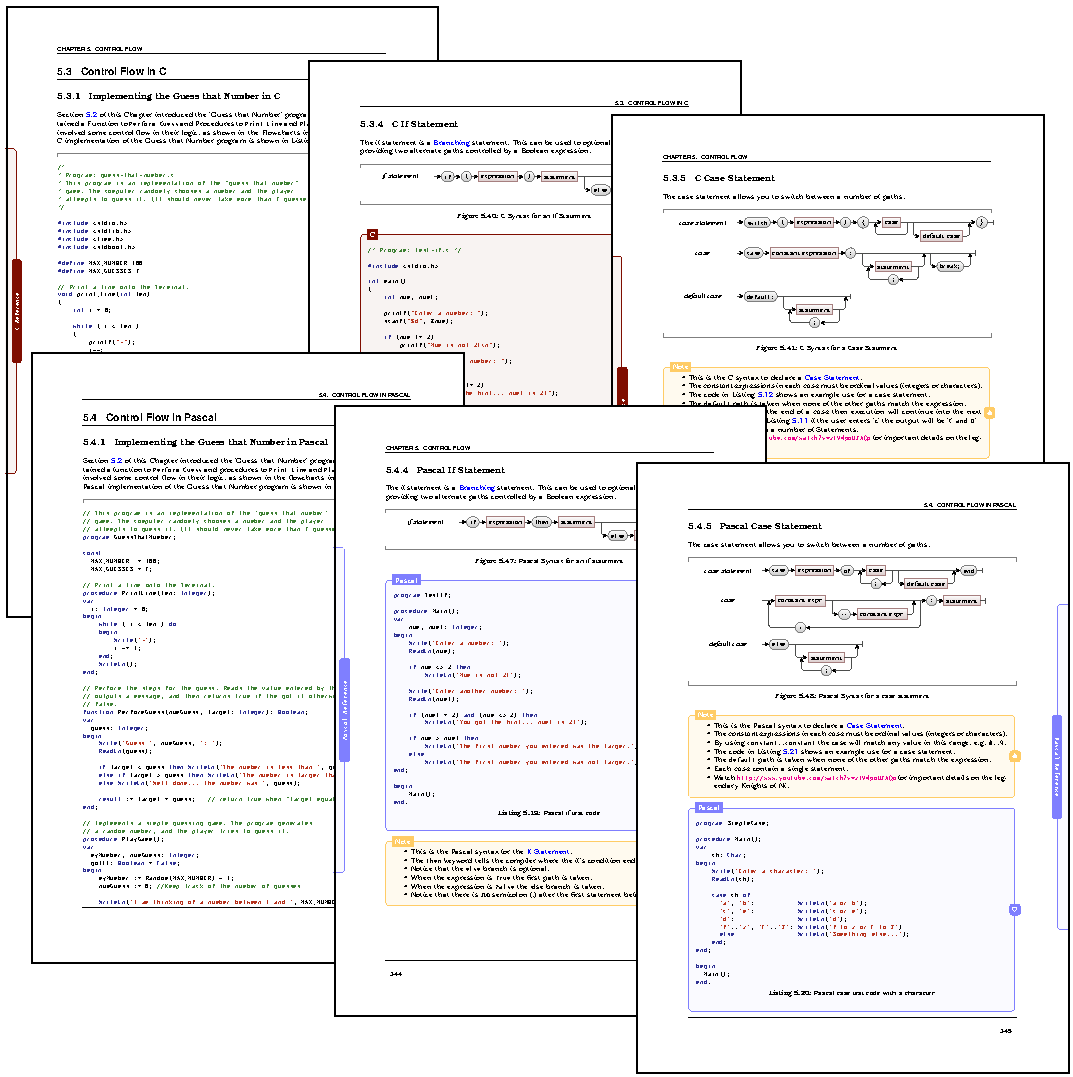
\includegraphics[width=0.7\textwidth]{ArcanaSyntax}
  \caption{Example pages from the Programming Arcana showing C and Pascal syntax and examples.}
  \label{fig:arcana_syntax}
\end{figure}

% paragraph syntax (end)

\clearpage

\paragraph{Understanding the Concepts:} % (fold)
\label{par:understanding_the_concepts_}

% paragraph understanding_the_concepts_ (end)

Programming has been likened to understanding how to control a notional machine \cite{DuBoulay:1986}. The notional machine represents an ideal computer in which the programming constructs being taught are realised. To help students realise the goal of controlling this machine, the next section of each chapter in the Programming Arcana provided a series of illustrations that tried to communicate the state and behaviour of the notional machine being presented. 

\fref{fig:arcana_understanding} shows some examples from the chapter on control flow. The illustration of the notional machine focuses on memory, and the instruction the computer is executing. Each instruction in the code is executed and explained on a single page.

\begin{figure}[h]
  \centering
  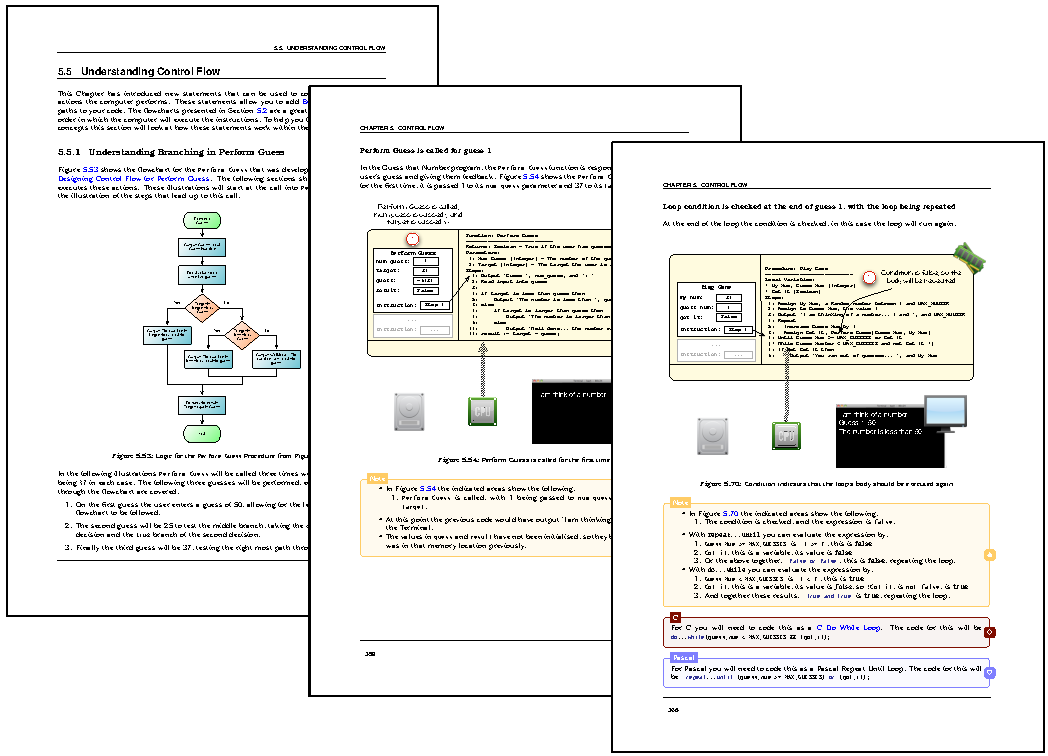
\includegraphics[width=0.8\textwidth]{ArcanaUnderstand}
  \caption{Examples of pages on how the concepts worked at a conceptual level in the machine from the Programming Arcana.}
  \label{fig:arcana_understanding}
\end{figure}

\clearpage

% \begin{figure}[p]
%   \centering
%   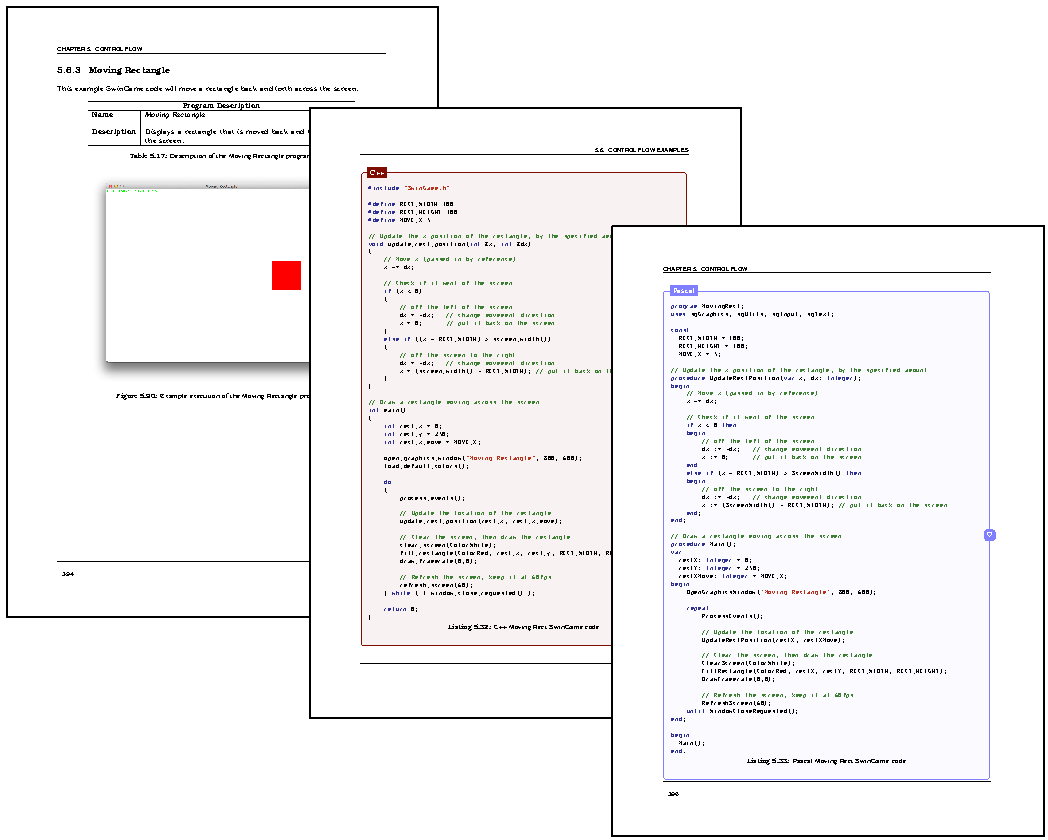
\includegraphics[width=0.8\textwidth]{ArcanaExamples}
%   \caption{Example code from the Programming Arcana.}
%   \label{fig:arcana_examples}
% \end{figure}


% subsubsection chapter_layout (end)


\subsubsection{Generating Railroad Diagrams} % (fold)
\label{ssub:railroad_diagrams}

Another aim in constructing the Programming Arcana was to provide students with descriptions of the programming language grammar. This could be achieved using a textual representation of the programming language grammar with the Backus Naur Form (BNF) \cite{Backus:1959} or the Extended Backus Naur Form (EBNF) \cite{Wirth:1977}. Instead, it was decided to use the ``Railroad diagrams'' described by \citet{Braz:1990}. These provide a more visual means of presenting the grammar, which was intended to be benefit people reading these diagrams for the purpose of writing programs.

To help automate the creation of the ninety syntax diagrams present in the programming arcana, a language translator was developed to convert grammars expressed textually into a graphical railroad diagram that could be included in the text and lecture slides. 

Originally, grammars expressed in BNF used recursion to implement the repetition of elements in the language. In proposing EBNF, \cite{Wirth:1977} included an iteration construct that reduced the heavy use of recursion for expressing simple repetition of elements in the language. To simplify the generation of railroad diagrams, EBNF was extended further to cater for repeated patterns that included a separator. In BNF and EBNF this can be achieved using recursion, whereas in the railroad diagram the separator should be placed on the returning arrow that implemented the loop. The syntax diagram in \fref{syn:paramlist} illustrates these two approaches. 

\syntax{syn:paramlist}{Examples of the declaration of a parameter list with recursion and without.}{paramlist}

To cater for the more flexible representation in the railroad diagrams, an extended version of EBNF was used. This extension added the ability to indicate a separator for repetitions, and to indicate if the repetition occurred at least once. The grammar for this extended version of EBNF is shown in its own form in \fref{lst:eebnf}, and as a railroad diagram in \fref{syn:eebnf}.

\ebnfsection{lst:eebnf}{Extended EBNF grammar in Extended EBNF}{\ebnfcode{syntax/eebnf.ebnf}}

\syntax{syn:eebnf}{Syntax for grammar used in language diagram generation.}{eebnf}

The \texttt{+ | *} after the repetition indicates either that the grammar had to be repeated one or more times (\texttt{+}) or zero or more times (\texttt{*}). The optional group following this indicated the presence of a separator, between each repetition of the grammar in the language. For example, the parameter list from \fref{syn:paramlist} could be coded as ``\texttt{param list = \{parameter\}+(",");}''.

This grammar was used to create all of the railroad diagrams for the Programming Arcana, and enabled syntax to be quickly expressed and documented for both C and Pascal.

% subsubsection railroad_diagrams (end)

\subsubsection{Summary} % (fold)
\label{ssub:arcana_summary}

The Programming Arcana demonstrates how the concept-based approach can be embedded down to the syntax level. The text provided students with details programming concepts, how they apply to code design, the associated syntax, and details on how they worked within the notional machine. A range of learning styles were supported through the presentation of the syntax and concepts using both images and text. 

% subsubsection summary (end)


% subsection programming_arcana (end)

\subsection{Video Podcasts} % (fold)
\label{sub:vodcasts}

% subsection vodcasts (end)

\subsection{Summary} % (fold)
\label{sub:arcana_summary}

% subsection summary (end)

% section itunesu_vodcasts_to_support_ (end)

\section{A Game Library to Support Procedures First} % (fold)
\label{sec:swingame}

SwinGame Documentation Website

Language translation



% section swingame_a_game_library_to_support_procedures_first (end)



% chapter supporting_the_curriculum (end)
%!TEX root = Constructive Alignment for Introductory Programming.tex

\chapter{Evaluation of the Teaching and Learning Context} % (fold)
\label{cha:evaluation}

\graphicspath{{Figures/Evaluation/}}

This chapter presents the results from a number of smaller studies into the effectiveness of the model presented in \cref{cha:approach}. The units analysed match those described in \cref{cha:example_impl}, and made use of the resources discussed in \cref{cha:supporting}. 

\sref{sec:research_design} describes the action research method, and thematic analysis approach, used in this work and outlines how the ethical issues related to analysing student work were addressed. This is followed by \sref{sec:lessons_learnt_from_action_research} that presents a discussion of the evolution of the model, and the associated resources and assessment criteria, across all iterations of the action research process. \sref{sec:issues_identified_in_student_reflections} and \sref{sec:evaluating_progress_using_burndown_charts} provide the results and discussions from the thematic analysis of student portfolios from two teaching periods. \sref{sec:issues_identified_in_student_reflections} discusses issues that students reported in their reflections, while \sref{sec:evaluating_progress_using_burndown_charts} examines student progress as depicted by the burn down charts from their portfolios. 

\section{Research Design} % (fold)
\label{sec:research_design}

\subsection{Action Research} % (fold)
\label{sub:action_research}

Due to the practical nature of this research, its focus on student learning, and the embedded reflective process it was decided to follow a Practical Action Research \cite{Creswell:2008} design based on Mills' \cite{Mills:2010} \emph{dialectic action research spiral}. This model, shown in \fref{fig:mills_spiral}, includes a four step process: (1) identify an area of focus, (2) collect data, (3) analyse and interpret the data, and (4) develop an Action Plan. %The Iterations section documents the \emph{focus}, \emph{plan}, \emph{data}, and \emph{analysis and reflections} per iteration.

\begin{figure}[htbp]
  \centering
  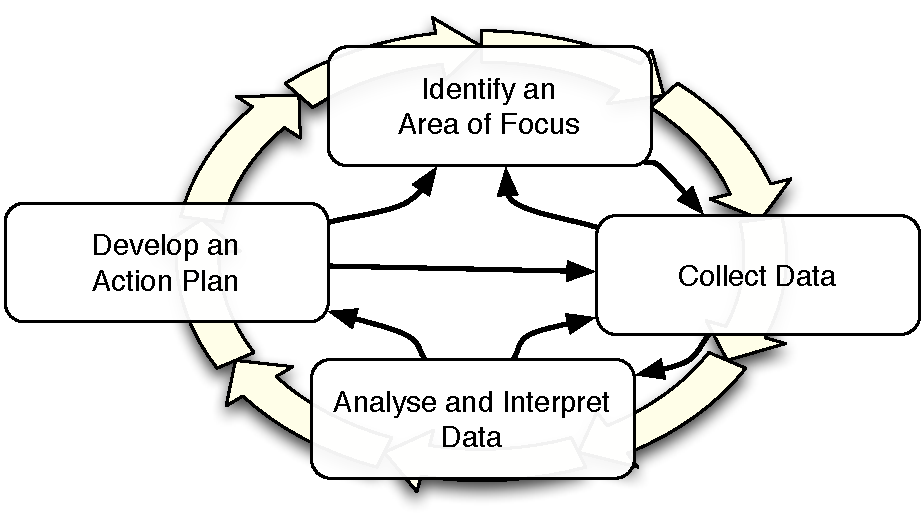
\includegraphics[width=0.7\columnwidth]{MillsSpiral}
  \caption{Mills \cite{Mills:2010} Dialectic Action Research Spiral.}
  \label{fig:mills_spiral}
\end{figure}

Iterations in this action research project aligned to teaching periods that included the delivery of one, or more, of the programming units discussed in \cref{cha:example_impl}. Each iteration included an \emph{action plan} related to implementing the approach from \cref{cha:approach}, which influenced the \emph{focus} for the iteration, the data collected, and the analysis performed.

The overall focus for this research was on the development, application and iterative improvement of the model from \cref{cha:approach}. The iterative nature of the action research process meant that the specific focus in each teaching period addressed relevant aspects of the model, based on its current state and feedback from previous iterations. 

Data collection included analysis of student portfolios, student grades, unit documentation and staff reflections, as illustrated in \fref{fig:research_data}. Each of these is described in the following paragraphs, with the ethical considerations related to using student work being discussed in \sref{sub:addressing_ethical_concerns}.

\begin{figure}[thb]
  \centering
  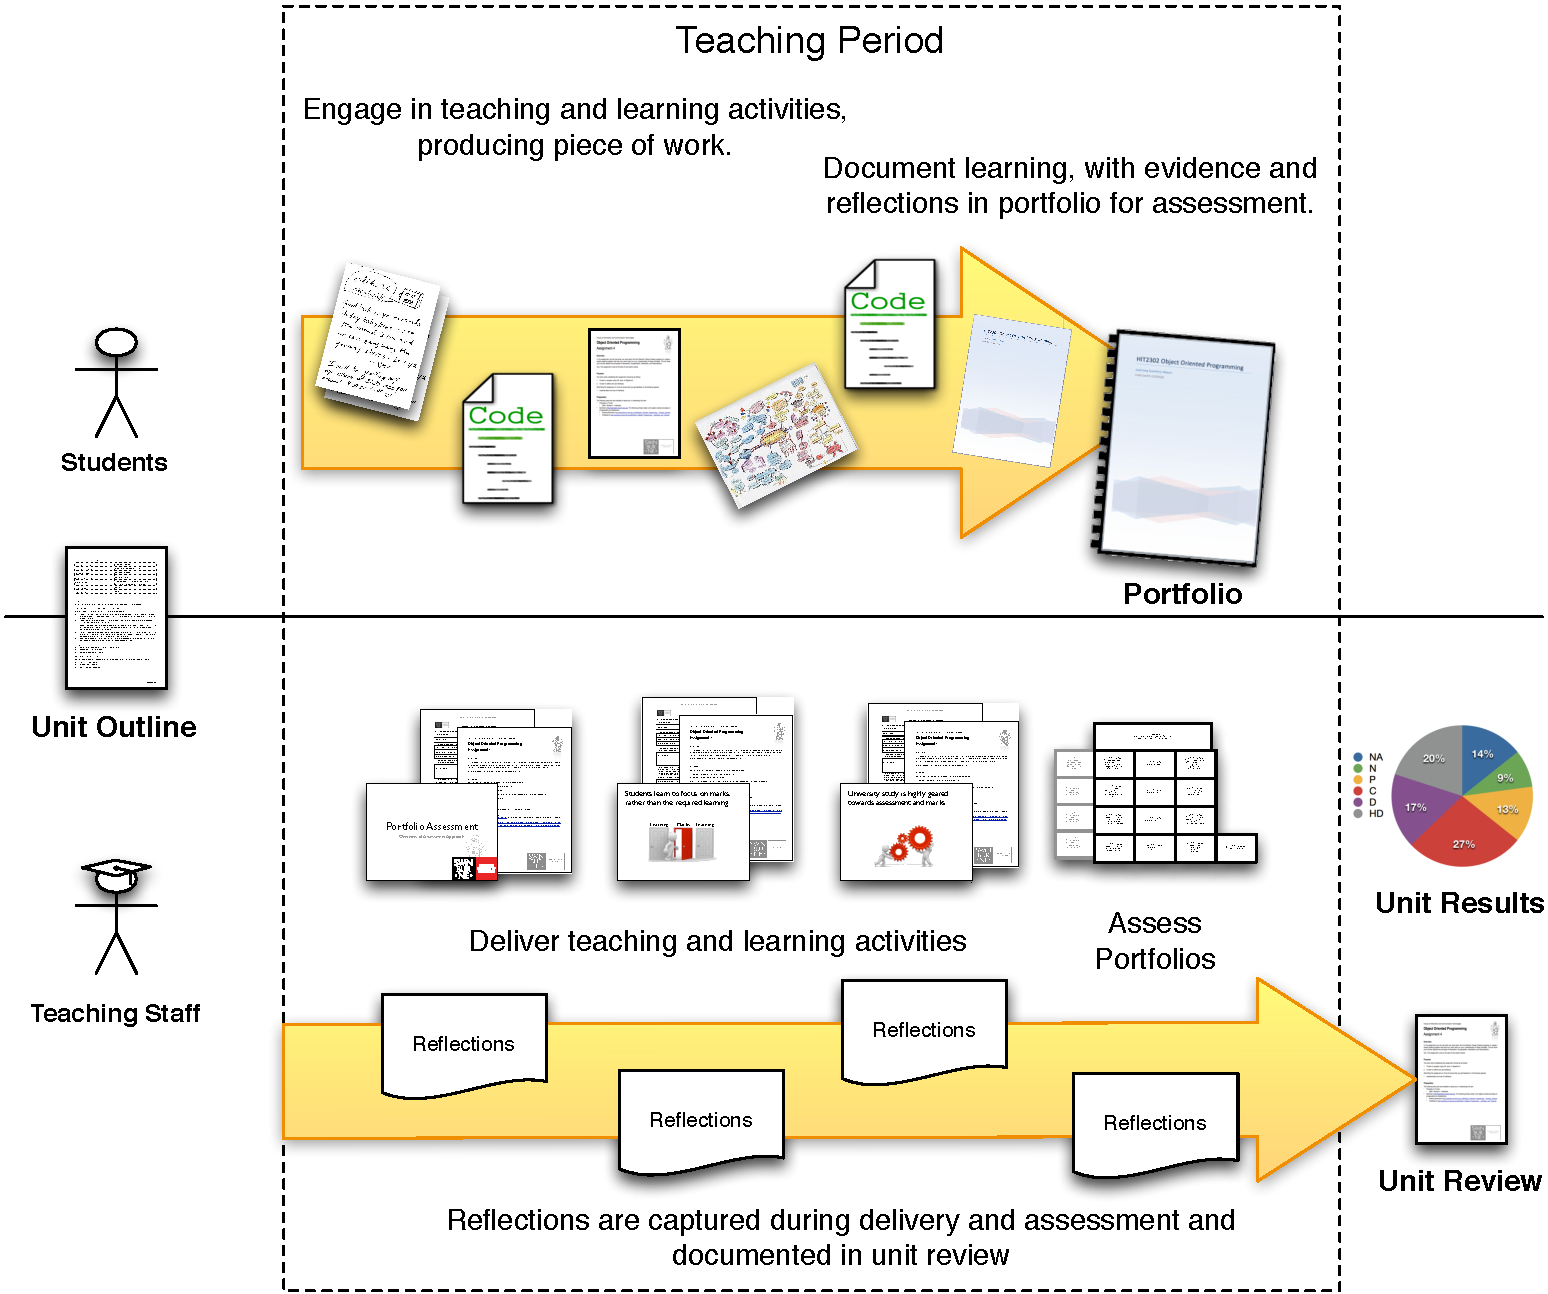
\includegraphics[width=\textwidth]{ResearchData}
  \caption{Illustration of the various documents used in the data collection for this research.}
  \label{fig:research_data}
\end{figure}

Thematic analysis was used to examine reflections in student portfolios, which is discussed further in \sref{sub:thematic_analysis}. As the thematic analysis of student portfolios was time consuming, it was not performed in all iterations. In teaching periods where a thematic analysis of the portfolios was not performed, the student grades and staff reflections provide insights into the composition of student portfolios.

Unit documentation included the Unit Outline and Unit Review documents. The Unit Outline included the intended learning outcomes and assessment criteria used in the given teaching period. This document was provided to students prior to the commencement of the teaching period and was an actively used document by both teaching staff and students. The Unit Review document was created after results were reported, and captured details of student perceptions of the teaching, teaching and learning approach, results, unit management, and any planned changes for future delivery of the unit. These documents were prepared by the Unit Panel, which included input from all teaching staff.

% The learning environment has been found to influence students' approach to learning \cite{Entwistle:1990,Entwistle:1991,Kember:2007}, and perceptions of these environments have been shown to directly, and indirectly, influence learning outcomes \cite{Meyer:1990,Lizzio:2002}. This research attempts to capture this using results from the University's student satisfaction surveys.

Staff reflections indicated the qualities exhibited in the student portfolios for a given semester. Staff reflections were captured both during the semester and after the portfolios were assessed. These reflections were recorded in notes, which in many cases were then summarised in the Unit Review document.

Student grades provide an indication of how well students performed in the given semester. Together with the staff reflections, these results provide insight into the learning outcomes students achieved - insights not available by considering students grades alone.

% subsection action_research (end)

\subsection{Thematic Analysis of Reflections} % (fold)
\label{sub:thematic_analysis}

Reflections in student portfolios provide a wealth of information. To help identify themes and patterns in the portfolios it was decided to perform a thematic analysis using the process outlined by \citet{Braun:2008}. This process involves six phases (with some terminology adapted for clarity):
\begin{enumerate}[noitemsep,nolistsep]
  \item Familiarising yourself with the data
  \item Generating initial themes,
  \item Searching for strong themes
  \item Reviewing themes
  \item Defining and naming themes
  \item Producing the report
\end{enumerate}

In each teaching period where a thematic analysis was performed, familiarity with the data was obtained early in the process with all portfolios being read as part of the unit assessment. At the end of the unit assessment, teaching staff made notes related to general issues, progress, and the overall quality of portfolios. This was part of standard unit delivery procedures, with the resulting reflections being summarised in the Unit Review document as mentioned in \sref{sub:action_research}.

Once the portfolios were made available for this research initial themes were generated by revisiting the reflective component of each portfolio and looking for the qualities under examination. These themes were then documented, and recorded in a spreadsheet. The spreadsheet software was used to collate the themes and record the portfolio details of where these issues had been mentioned, along with any illustrative comments using the students own words.

In phases 3 through 5 the identified themes were broadly grouped together, and then each broad group was examined for sub-themes. All of the themes identified in the examination of student portfolios were maintained in the final categorised results. Themes that did not clearly relate to any of the identified groups were grouped together as a miscellaneous group.

In the reporting of this analysis we present the raw results, grouped into the identified themes. Illustrative quotes from the student reflections are provided to help define the themes.

% subsection thematic_analysis_of_reflections (end)


\subsection{Addressing Ethical Concerns} % (fold)
\label{sub:addressing_ethical_concerns}

Participants in this study were students of the investigators, and so it was important to design an appropriate process whereby students could offer informed consent to participate in the research with no risk of coercion. The student-teacher relationship was the main source of potential ethical problems for this research, with perceptions of coercion being the central concern. 

This issue is further complicated by the fact that the researchers may teach both the first and second programming units, for example students may undertake the introductory programming unit in the first half of the year, and the object oriented programming unit in the second half of the year. As most students who complete the first unit progressed to the second unit the following semester, there was the potential for the perception of coercion in this second unit.

An appropriate research protocol was developed, and given ethical approval from Swinburne's Human Research Ethics Committee. \fref{fig:ethics_process} shows an overview of this process. 

\begin{figure}[thb]
  \centering
  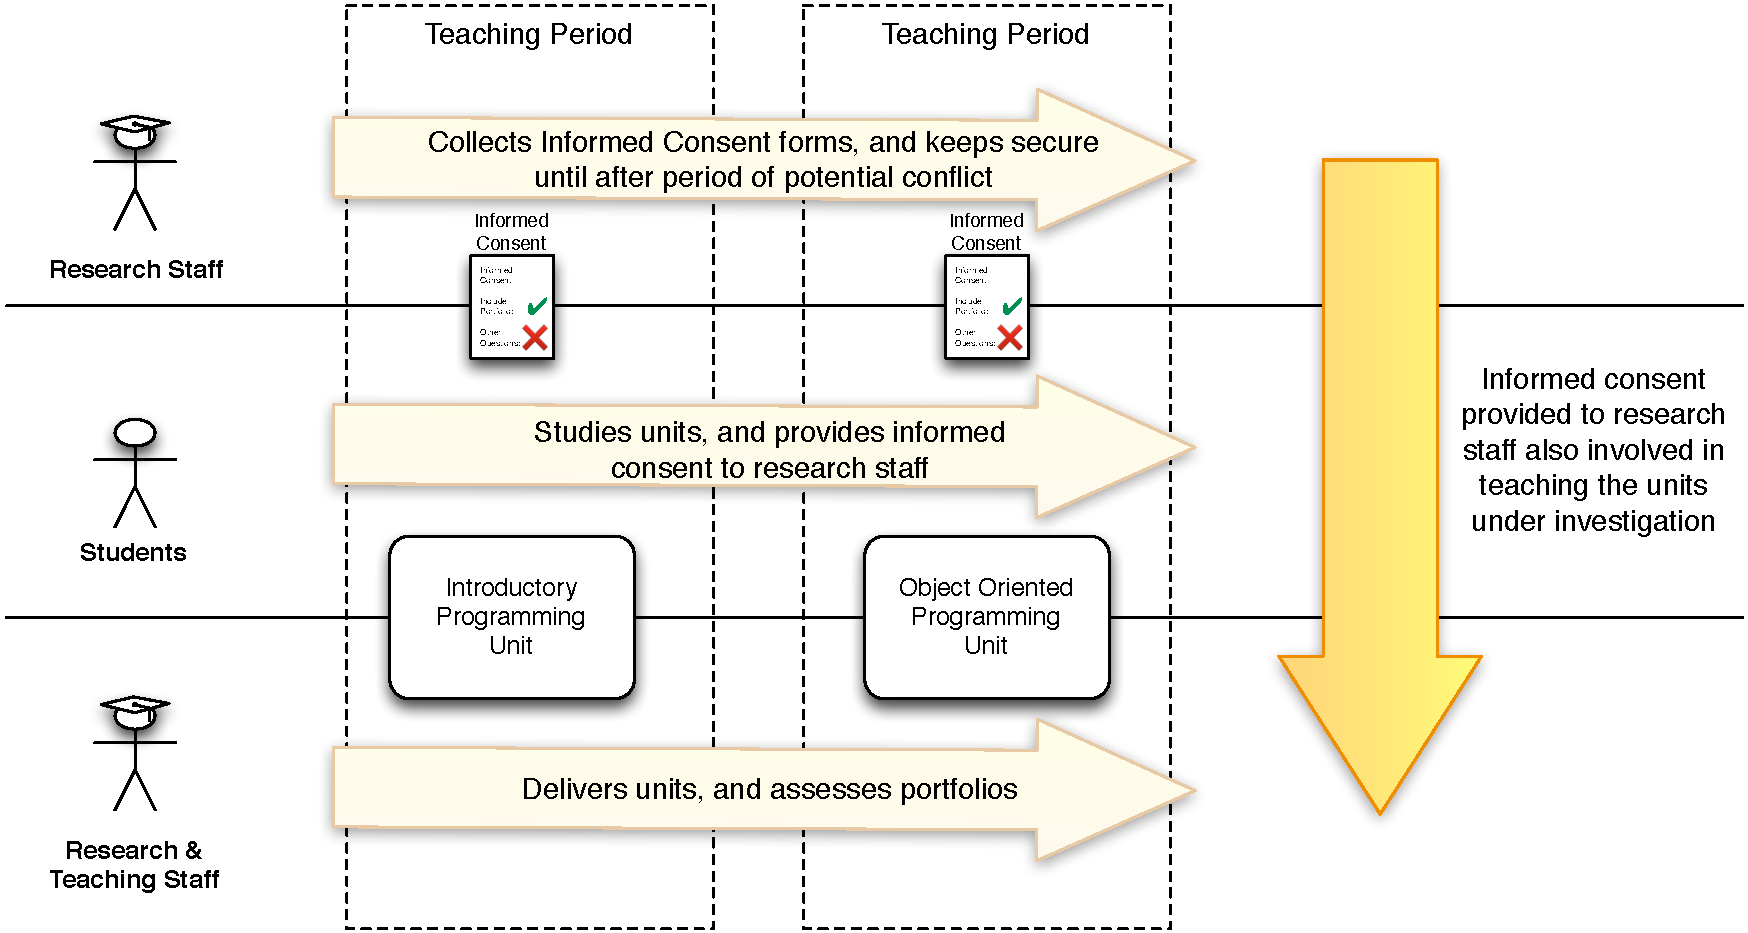
\includegraphics[width=\textwidth]{EthicsProcess}
  \caption{Overview of the process to avoid perceptions of coercion. Informed Consent forms were completed by students in both the introductory programming and object oriented programming units. These forms are collected by researchers not directly involved in the teaching of the unit. The informed consent forms are only made available to the staff involved in teaching the unit after the both units are complete.}
  \label{fig:ethics_process}
\end{figure}

Printed Informed Consent forms were distributed to students in lectures during the teaching period. The forms were completed by all students, and indicated their willingness to have their work included in the research. Students were informed that participation in the research was voluntary, and their response would in no way influence their results or relationship with the university.

To avoid any perception that student responses could in any way affect their results, the Informed Consent forms were withheld from researchers involved in teaching these students until the period of potential influence was deemed to have passed. Until such time, the forms were kept in a sealed envelope in a locked cabinet at Swinburne by the researchers who were not directly involved in teaching of the units. Additionally, all students were required to complete and sign the forms, indicating if they wished to participate or not. In this way it was not be possible to determine those who did, or did not, wish to participate simply by observing those who sign the form.

% \begin{itemize}[noitemsep,nolistsep]
	% \item The Unit Summary Survey was voluntary and anonymous. No identifying information was collected within the questionnaire and there was no means of matching responses with individual students.
	% \item The informed consent forms that indicated if students were willing to have their responses to the Initial Survey and their Portfolio work (for the thematic analysis) included in this research were withheld from researchers involved in teaching these students until the period of potential conflict was deemed to have passed. Until such time, the forms were kept in a sealed envelope in a locked cabinet at Swinburne by the researchers who were not directly involved in teaching of the units. 
	% \item The informed consent forms that indicated if students were willing to have their Portfolio work included in this research (for the thematic analysis) were withheld from researchers involved in teaching these students until the period of potential conflict was deemed to have passed. Until such time, the forms were kept in a sealed envelope in a locked cabinet at Swinburne by the researchers who were not directly involved in teaching of the units. 
	% \item Additionally, all students were required to complete and sign the forms, indicating if they wished to participate or not. In this way it was not be possible to determine those who did, or did not, wish to participate simply by observing those who sign the form.
	% \item The Focus Group will be organised and run by researchers not involved in the teaching and assessment of the unit. Data from the Focus Groups will be transcribed into an encoded form using an encoding scheme whereby the student names and ids will not be known by researchers involved in teaching the units until after the period of potential conflict is deemed to have passed. After this period has passed the same encoding scheme will be used to encode responses to the Initial Survey, Progress Surveys, and data collected from the Thematic Analysis.
% \end{itemize}

The period of potential influence was deemed to have passed based on the following:
\begin{itemize}[noitemsep,nolistsep]
	\item For the introductory programming units where the researchers were not involved in teaching a follow on unit, the period of potential influence was deemed to have passed once the results for the introductory programming unit were published.
	\item For the introductory programming units where the researchers were involved in the teaching the follow on unit, the period of potential influence was deemed to have passed once the results for the \emph{second} unit were published.
	\item For the object oriented programming units, the period of potential influence will be deemed to have passed once the results for the unit were published.
\end{itemize}

% subsection addressing_ethical_concerns (end)

% section research_design (end)

\section{Lessons Learnt through Action Research} % (fold)
\label{sec:lessons_learnt_from_action_research}

The action research process was used in the development, application, and evaluation of the model presented in \cref{cha:approach}. A total of nine iterations were completed over a five year period, involving thirteen unit deliveries, with a total of 983 portfolios assessed. This section reports on the development of the model, its guiding principles, the teaching an learning activities and supporting resources.

\subsection{The Units} % (fold)
\label{sub:the_units}

\cref{cha:example_impl} presented details of two example implementations of the model. These examples represent the current status of this research, which evolved iteratively from the delivery of four separate programming units: two introductory programming units, and two object oriented programming units. \tref{tbl:units_iteration} shows the four different programming units, and the iterations in which they were involved. All of the units were taken by undergraduate students early in their degree programme and were convened by the author. General details of the four units follow, and any changes to individual iterations are presented in the following sections.

\begin{table}[htb]
  \footnotesize
  \renewcommand{\arraystretch}{1.3}
  \caption{Units in each iteration.}
  \label{tbl:units_iteration}
  \centering
	\begin{tabular}{l|c|c|c|c|c|c|c|c|c|c}
 		%\hline
		Units \textbackslash{} Iteration & 1 & 2 & 3 & 4 & 5 & 6 & 7 & 8 & 9 & Current \\ \hline
		Introductory Programming (A) & \checkmark & ~ & \checkmark & ~           & \checkmark & \checkmark & ~           & \checkmark & ~ & \checkmark           \\ 
		Introductory Programming (B)    & ~           & ~           & ~           & ~           & ~           & ~           & \checkmark & \checkmark & \checkmark & \checkmark \\ \hline
		Object Oriented Programming (A) & ~           & \checkmark & ~           & \checkmark & ~           & ~           & \checkmark & ~           & \checkmark & \checkmark \\ 
		Object Oriented Programming (B) & ~           & ~           & ~           & ~           & ~           & ~           & ~           & ~           & \checkmark & \checkmark
		%\hline
	\end{tabular}
\end{table}

\subsubsection{Introductory Programming (A)} % (fold)
\label{ssub:introductory_programming_a}

Introductory Programming (A) was taken by students in their first semester and introduced them to procedural programming, as outlined in \cref{cha:example_impl}. The intended learning outcomes included the ability to read and interpret code, write small procedural programs, iteratively use modular and functional decomposition to break problems down, and the ability to apply the principles of structured programming (focusing on blocks of code and using sequence, selection, and repetition). Outcomes were expressed in a language neutral manner as the focus of the unit was on the underlying programming concepts.

Introductory programming (A) was taken by students studying a range of degrees. Most students were enrolled in a Bachelor of Science, majoring in Computer Science, Professional Software Development or Games Development.

% subsubsection introductory_programming_ (end)

\subsubsection{Object Oriented Programming (A)} % (fold)
\label{ssub:object_oriented_programming_a}

Object Oriented Programming (A) had Introductory Programming (A) as a prerequisite and was predominantly taken by students in their second semester. As outlined in \cref{cha:example_impl}, the intended learning outcomes in this unit required students to design, develop and test object oriented programs, as well as communicate the underlying principles of abstraction, encapsulation, inheritance and polymorphism. As with Introductory Programming (A), the outcomes were expressed in a language neutral manner and the focus was on underlying concepts.

The student cohort in Object Oriented Programming (A) consisted only of students that had completed Introductory Programming (A).

% subsubsection object_oriented_programming_ (end)

\subsubsection{Introductory Programming (B)} % (fold)
\label{ssub:introductory_programming_b}

Prior to iteration seven this unit was taught using a textbook style approach with assignments and a final exam. In iteration seven the unit was adapted to a portfolio-based approach, and then combined with Introductory Programming (A) from iteration eight.

Intended learning outcomes for Introductory Programming (B) covered similar topics to Introductory Programming (A) but with specific reference to the C programming language. When this was combined with Introductory Programming (A) in iteration eight, the combined outcomes matched those from \cref{cha:example_impl}, and the focus shifted from language syntax to programming concepts.

The cohort of Introductory Programming (B) included students from a range of degree programmes. This included students studying for a Bachelor of Information and Communication Technology, Bachelor of Engineering and Bachelor of Science (Computer Science and Software Engineering). The unit was included in a number of other degrees as an elective.

% subsubsection introductory_programming_ (end)

\subsubsection{Object Oriented Programming (B)} % (fold)
\label{ssub:object_oriented_programming_b_}

As with Introductory Programming (B), Object Oriented Programming (B) was taught using a specific language (C++), used a textbook style approach, traditional assignments and final exam. This unit covered the same topics as Object Oriented Programming (A), and in iteration nine the two object oriented programming units were combined into a single unit. This combined unit used portfolio assessment and its intended learning outcomes matched those from \cref{cha:example_impl}, and focused on programming concepts and principles. Students continued to enrol in the individual units, but were taught as a single cohort. Students enrolled in Object Oriented Programming (B) were required to include evidence in their portfolios of being able to apply the unit's concepts using the C++ language.

% subsubsection object_oriented_programming_b_ (end)

\subsubsection{Relationship Between Units} % (fold)
\label{ssub:relationship_between_units}

\fref{fig:unit_paths} shows progression paths through these units. The students we broadly classified as having a \emph{software development} focus took Introductory Programming (A) in the first semester of their first year, and then Object Oriented Programming (A) in the second semester of their first year. Introductory Programming (B) was taken primarily by Engineering students, who subsequently took an intermediate programming unit before studying Object Oriented Programming (B). For the Engineering students, this sequence may be extended over more than three consecutive semesters depending on their degree programme.

\begin{figure}[htbp]
  \centering
  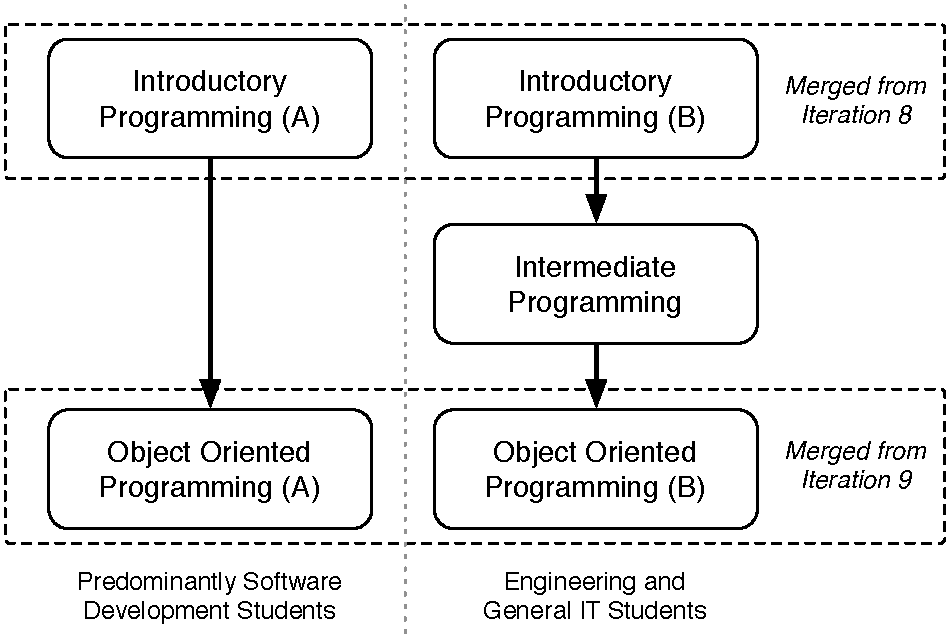
\includegraphics[width=0.8\textwidth]{UnitPaths}
  \caption{Progression pathways through the introductory programming units.}
  \label{fig:unit_paths}
\end{figure}

% subsubsection relationship_between_units (end)
% subsection the_units (end)


% cohort
% grade distributions
% student evaluations
% portfolio contents - by grade
% use of SwinGame
% general themes from portfolios
% depth of approach to learning

\subsection{Early Iterations} % (fold)
\label{sub:early_iterations}

\subsubsection{Iteration 1} % (fold)
\label{sub:iteration_1}

\paragraph{Focus} % (fold)

This was our first attempt at portfolio assessment, and so the focus for the first iteration was on implementing portfolio assessment in general. Most of our attention was on implementing changes in line with constructivist learning theories, \pref{itm:construct} from \cref{cha:guiding_principles}.

\paragraph{Action Plan} % (fold)

The approach used was an iterative step toward the general model presented in \cref{cha:approach}. Students were required to complete six assignments and six tests, with the \emph{option} to include a portfolio. The aim of the assessment strategy was for students to demonstrate their understanding of core concepts in the assignments and tests, with the portfolio used to determine student ability in the higher grade brackets. Appropriate weights were applied to each of the assessment items and these were added together to calculate the final grade.

Key differences from the portfolio model presented in \cref{cha:approach}:
\begin{itemize}[noitemsep,nolistsep]
  \item The unit included a total of eleven intended learning outcomes, each making use of active verbs and relating to specific parts of the unit.
  \item It used multiple assignments (six) over the semester.
  \item It included tests that were marked and contributed to the final grade.
  \item Submission of a portfolio was optional.  All students who submitted a portfolio were interviewed.
\end{itemize}

Similarities with later portfolio iterations included:
\begin{itemize}[noitemsep,nolistsep]
  \item It included criteria for each grade, though these were described in general terms.
  \item Students included a self assessment against the criteria.
\end{itemize}

Key differences from the introductory programming unit described in \cref{cha:example_impl} included the following:
\begin{itemize}[noitemsep,nolistsep]
	\item Focus was on programming concepts, but there was more crossover of topics in the early material.
	\item The teaching and learning activities made limited use of SwinGame.
	\item Procedures were introduced later, as SwinGame was not used in the early parts of the teaching period. 
	\item Students were only briefly introduced to the C programming language at the end of the unit.
	\item None of the supporting tools from \cref{cha:supporting} had been developed at this stage.
	\item Lecture slides closely followed the ``Beyond Bullet Points'' approach \cite{Atkinson:2007}, and included extensive notes on each slide.
	\item An earlier edition of the Pascal Language Reference \cite{FPC:2013lang} was used as the unit text.
\end{itemize}

\paragraph{Data} % (fold)

Unit results across all iterations are shown in \tref{tbl:unit_results}. This lists the number of students receiving each grade over the nine iterations. Grades include those students who enrolled but did not submit a portfolio (NA) those who failed (N) and those who received Pass (P) Credit (C) Distinction (D) and High Distinction (HD) result. The results for Iteration 1 are shown in \fref{fig:iterations_1_2}. In this iteration a large percentage of students managed to receive an HD grade.

\begin{table}[p]
  \footnotesize
  \renewcommand{\arraystretch}{1.3}
  \caption{Unit Results Across Iterations 1 to 9 for the introductory programming and object oriented programming units.}
  \label{tbl:unit_results}
  \centering
    \begin{tabular}{l|l|c|c|c|c|c|c}
        Iter. & Unit    & NA & N  & P  & C  & D  & HD \\ \hline
        1         & Introductory Programming (A)  & 3  & 1  & 4  & 5  & 6  & 11 \\ \hline
        2         & Object Oriented Programming (A) & 19 & 7  & 14 & 19 & 13 & 11 \\ \hline
        3         & Introductory Programming (A)  & 9  & 1  & 2  & 9  & 6  & 9  \\ \hline
        4         & Object Oriented Programming (A) & 4  & 7  & 3  & 17 & 6  & 5  \\ \hline
        5         & Introductory Programming (A)  & 10 & 6  & 9  & 19 & 12 & 14 \\ \hline
        6         & Introductory Programming (A)  & 14 & 3  & 28 & 20 & 14 & 5  \\ \hline
        7         & Introductory Programming (B)  & 42 & 12 & 56 & 47 & 22 & 7  \\ 
        ~         & Object Oriented Programming (A) & 5  & 8  & 18 & 10 & 8  & 9  \\ \hline
        8         & Introductory Programming (A)  & 11 & 5  & 20 & 21 & 17 & 14 \\ 
        ~         & Introductory Programming (B)  & 39 & 47 & 84 & 36 & 20 & 9  \\ \hline
        9         & Introductory Programming (B)  & 61 & 4  & 78 & 24 & 25 & 7  \\ 
        ~         & Object Oriented Programming (A) & 14 & 0  & 25 & 6  & 14 & 7  \\ 
        ~         & Object Oriented Programming (B) & 7  & 0  & 25 & 5  & 3  & 4  
    \end{tabular}
\end{table}

\begin{figure}[p]
  \centering
  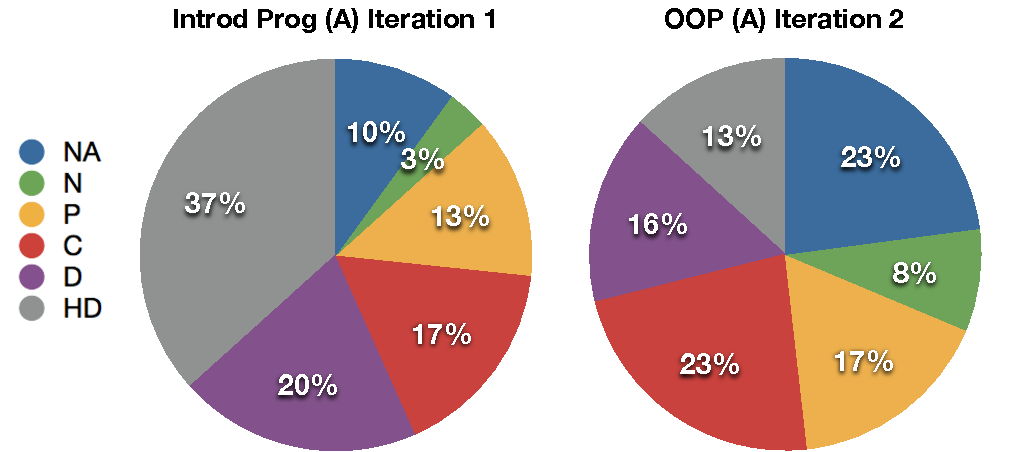
\includegraphics[width=0.8\columnwidth]{Iterations1_2}
  \caption{Result distributions from Iterations 1 and 2.}
  \label{fig:iterations_1_2}
\end{figure}

\paragraph{Reflections and Analysis} % (fold)
\label{ssub:analysis}

Staff reflections included several interesting aspects related to the assessment in this iteration:
\begin{itemize}[noitemsep,nolistsep]
  \item There were too many intended learning outcomes. This had made it difficult for staff to clearly communicate how teaching and learning activities related to the outcomes. Students had also found it difficult to relate their portfolio pieces back to the intended learning outcomes.
  \item Criteria were difficult to apply, being weakly defined, and students tended to weaken the criteria further in their self assessment.
  \item Significant effort had been put into creating ``Beyond Bullet Point'' slides and associated notes, which had been useful in terms of delivery but were restricting opportunities to adapt the material.
  \item Assessing the portfolios was very time consuming.
  \item Staff felt confident that a portfolio of work would provide a suitable means of assessing student outcomes in technical units.
  \item Core assignments and tests:
  \begin{itemize}[noitemsep,nolistsep]
    \item Covered the minimum expectations for the intended learning outcomes.
    \item Received high marks, which only indicated basic coverage of the intended learning outcomes. 
  \end{itemize}
  \item Students with weak portfolios were still able to received high grades.
\end{itemize}

Use of portfolios was limited in this iteration, with positive and negative results. The two main issues were the weakness of the expressed assessment criteria and the combining of results from the assignments and tests. Together, these issues resulted in many students receiving a higher grade than staff felt was appropriate given the outcomes demonstrated in student portfolios. This is supported by the high portion of students with HD grades.

Positive aspects of the unit delivery included the improved confidence of staff in the potential for using portfolio assessment in units related to software development. Overall, it was felt that portfolio assessment offered great potential, but that this iteration had not managed to create a suitable environment in which these benefits could be realised.

\paragraph{Development of Principles} % (fold)

The first experience of delivering a portfolio assessed unit had been informed by examining the principles of constructive alignment, and the experience provided a number of insights that helped form the principles from \cref{cha:guiding_principles}. These included:

\begin{itemize}[noitemsep,nolistsep]
	\item Constructive learning theories, \pref{itm:construct}, and aligned curriculum, \pref{itm:align}, had been at the centre of this experience. The utility of both had been hampered by the large number of intended learning outcomes. This guided the importance of having a small number of more highly targeted outcomes.
	\item The portfolios had been able to capture student outcomes, but results had been impacted by the use of grades to encourage during the semester. While alternative schemes could have been developed, it was felt these incentives were not required and a greater use of formative feedback would have benefited the students. This emphasis on formative feedback evolved into \pref{itm:formative} and influenced a change from a soft Theory X to Theory Y, \pref{itm:theory_y}.
	\item Teaching staff were \emph{willing to change}, and wanted to be able to adjust teaching material in response to student issues. However, the significant effort that had gone into the develop of the ``Beyond Bullet Points'' lecture slides provided unproductive resistance to change. This conflict started a change in attitude that resulted in the definition of \pref{itm:agile}, the aim to be both \emph{agile} and \emph{willing to change}.
\end{itemize}

% paragraph development_of_principles (end)

% subsection iteration_1 (end)

\subsubsection{Iteration 2} % (fold)
\label{sub:iteration_2}

\paragraph{Focus} % (fold)

Iteration 2 included the delivery of Object Oriented Programming (A), and aimed to address several of the main concerns from Iteration 1: having \emph{fewer intended learning outcomes} around which everything would be based, assessing each student's outcomes as a whole with \emph{100\% portfolio assessment}, and \emph{specific assessment criteria} expressing what was expected for each grade. In addition to this, the unit material was separated into teaching and learning activities and teaching and learning resources, in an effort to enable greater flexibility with future changes.

\paragraph{Action Plan} % (fold)
\label{ssub:develop_an_action_plan2}

In this iteration the following aspects of our model were included:
\begin{itemize}[noitemsep,nolistsep]
  \item We adjusted the unit to use five intended learning outcomes.
  \item Assessment criteria were developed for each grade using the different levels from the SOLO taxonomy \cite{Biggs:1982}. This was presented in a format similar to that shown in \fref{fig:assessment_criteria}, though some details differed.
  \item Feedback was provided using weekly formative assessments, and tests.
  \item Notes previously embedded in slides were shifted to a single document and distributed to students as a PDF.
\end{itemize}

The following aspects differed:
\begin{itemize}[noitemsep,nolistsep]
  \item Each intended learning outcome had criteria for meeting it to differing standards: Marginal, Adequate, Good, and Excellent.
  \item A Credit grade required three intended learning outcomes to be addressed at an \emph{Adequate} standard, Distinction required two at a \emph{Good} standard (with all other adequate) and High Distinction required two \emph{Excellent} and all others \emph{Good}.
  \item A flipped classroom model \cite{Baker:2000,Lage:2000} was adopted: student were provided with online videos covering the weekly lecture material and class room activities were predominantly interactive.
\end{itemize}

Key differences from the object oriented programming unit described in \cref{cha:example_impl} included the following:
\begin{itemize}[noitemsep,nolistsep]
	\item A greater emphasis was placed on constructive learning theories, and a shift toward discovery learning. Concepts were presented using the video podcasts, and lecture activities included a greater emphasis on group discussions.
	\item Lectures used a number of interactive quizzes, questions were typically taken then discussed in groups and retaken to see changes in understanding.
	\item Laboratory exercises also had less guidance, and students explored their chosen language and how it could be used to implement object oriented programs.
	\item While multiple languages were used, and students could only choose between the Java and C\# programming languages.
	\item SwinGame was introduced early on to enable students to visualise object interactions through the creation of a drawing program.
\end{itemize}

% subsubsection develop_an_action_plan (end)

\paragraph{Data} % (fold)
\label{ssub:data2}

\fref{fig:iterations_1_2} shows the result distributions for Object Oriented Programming (A) in Iteration 2. The number of High Distinction results was closer to expectations, though the pass rate was a cause for concern. 

\paragraph{Reflections and Analysis} % (fold)
\label{ssub:staff_reflections_and_analysis2}

Key staff reflections included:
\begin{itemize}[noitemsep,nolistsep]
  \item Interviewing all students meant that portfolio assessment was very time consuming.
  \item The general structure of the assessment criteria was suitable, but there was a disconnect in perceived standard: the interpretation of ``good'' was significantly different between staff and students.
  \item Work was of a weaker standard than desired across all grades.
  \item Students did not benefit from the classroom flip, with few preparing adequately for the classroom discussions.
  \item It was felt that many students ``coasted'' along, and did not genuinely attempt the planned activities.
  \item Progress on understanding weekly topics was very slow, with the lack of guidance resulting in students not making the best use of their time.
  \item Separation of teaching and learning activities and resources had enabled a greater freedom in creating the interactive lecture, and the resources could be reused for future unit deliveries.
\end{itemize}

Staff felt that most of the issues from the semester could be attributed to the shift toward non-productive ``discover learning'' \cite{Anderson:1998}. In our effort to implement constructive learning theories we had reduced the amount of guided learning activities, and student productivity appeared to have been adversely affected.

It was still felt that portfolio assessment could be beneficial but that, again, we had failed to realise any benefits. In many ways, the results, in terms of student learning outcomes, from this teaching period had felt like a backward step.

\paragraph{Development of Principles} % (fold)

The teaching and learning environment created in Iteration 2 had been informed by the constructive learning theories, and a trusting Theory Y environment. At the end of this iteration it was felt that the Theory Y attitude was still appropriate, but that the overly zealous application of constructive learning theories had meant students were unable to appropriately apply themselves. The lack of guidance had resulted in many students spending too much time working out what it was they needed to learn, and not enough time applying the concepts related to object oriented programming.

This experience influenced a number of the principles from \cref{cha:guiding_principles}. 

\begin{itemize}[noitemsep,nolistsep]
	\item Constructive learning theories, central to \pref{itm:construct}, were tempered to include stronger guidance along with the focus on the central role of the learning in constructing their own knowledge. 
	\item We needed to more clearly communicate our high expectations of students, which became \pref{itm:expectations}. In this iteration many students did not seem to be aware of what had been expected of them.
	\item The shallow responses of students also indicated the need to focus on depth of understanding, \pref{itm:depth}.
\end{itemize}

% subsubsection iteration_2 (end)

% subsection early_iterations (end)

\subsection{As the Model Stabilised} % (fold)
\label{sub:as_the_model_stabilised}

Iterations 1 and 2 had hinted at the potential for portfolio assessment, but the implementation had been unsuccessful. The changes to the model at the end of Iteration 2 resulted in a more successful application of portfolio assessment, and Iterations 3 to 6 all applied the model in a similar way. 

\subsubsection{Iterations 3 to 6} % (fold)
\label{ssub:iterations_3_to_6}

\paragraph{Focus} % (fold)
\label{ssub:focus_3_6}

The focus of Iterations 3 to 6 was on both extended how we taught the units, and developing resources to support what we taught. In relation to how we taught, the focus was on the development of assessment criteria, with the aim to ensure these were clear for both staff and students, and could be applied efficiently to assess student outcomes. At the same time, each iteration worked on extending the resources available to support what we taught.

% subsubsection focus (end)

\paragraph{Action Plan} % (fold)
\label{ssub:plan_3_6}

Assessment criteria in each iteration adopted the changes from prior iterations, and made improvements to wording to better capture staff intentions for each grade criteria. An example of the overall assessment criteria is shown in \fref{fig:i6_assessment_criteria}, and details of the assessment criteria related to an individual intended learning outcome is shown in \fref{fig:i6_assessment_criteria_detail}.

Specific changes included: 
\begin{enumerate}[noitemsep,nolistsep]
  \item Iteration 3:
  \begin{itemize}[noitemsep,nolistsep]
    \item Adjusted the main category descriptors to: Adequate, Good, Outstanding, and Exemplary.
    \item The classroom flip was dropped, with videos now being used to support classroom activity.
    \item A reflective report was added that included the self assessment: an alignment of the pieces to the intended learning outcomes, and general reflections.
  \end{itemize}
  \item Iteration 4:
  \begin{itemize}[noitemsep,nolistsep]
    \item Reduced the number of items expected for each grade: Credit required one Good, Distinction one Good another Outstanding, and High Distinction required one Good another Outstanding and a further one at Exemplary.
  \end{itemize}
  \item Iteration 5:
  \begin{itemize}[noitemsep,nolistsep]
    \item Pass and Credit students were no longer interviewed.
    \item Tests became a hurdle requirement, and had to be completed to a satisfactory standard for students to be eligible to pass the unit.
  \end{itemize}
  \item Iteration 6:
  \begin{itemize}[noitemsep,nolistsep]
  	\item Short reports that discussed aspects related to each intended learning outcome were required to meet the \emph{Good} standard.
    \item To meet the \emph{Outstanding} standard for an intended learning outcome, students were required to develop a program of their own design and relate this to that intended learning outcome.
    \item Meeting the \emph{Exemplary} standard required a research report related to the intended learning outcome. 
  \end{itemize}
\end{enumerate}

\begin{figure}[p]
	\centering
	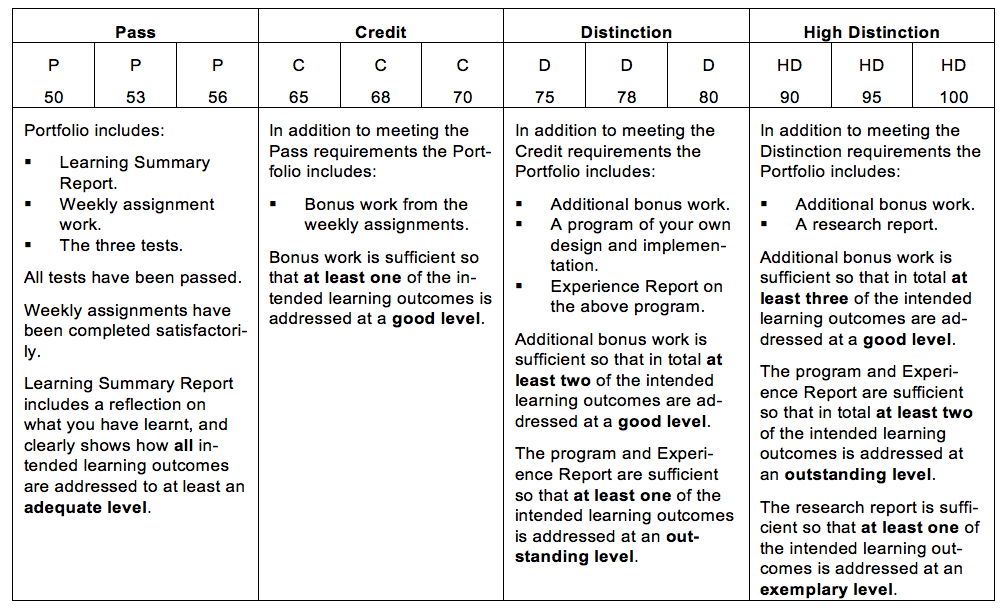
\includegraphics[width=\textwidth]{AssessmentCriteria}
	\caption{Overview of assessment criteria provided to students in the unit outline of Introductory Programming (A) in Iteration 6.}
	\label{fig:i6_assessment_criteria}
\end{figure}

\begin{figure}[p]
	\centering
	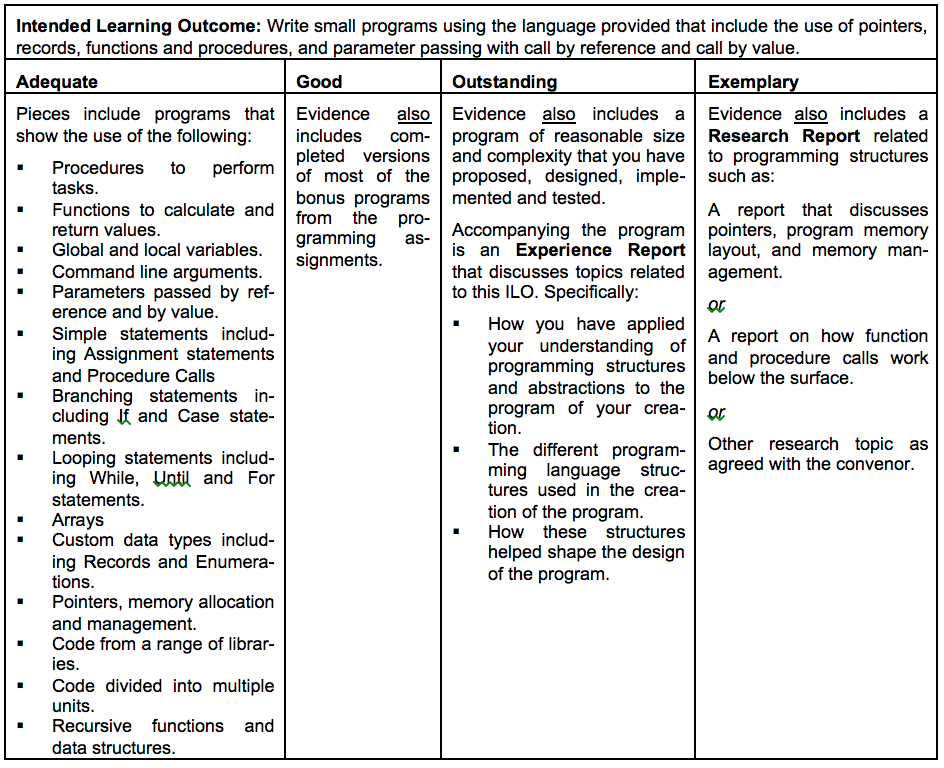
\includegraphics[width=1\textwidth]{AssessmentCriteriaDetail}
	\caption{Example assessment criteria related to a single intended learning outcome.}
	\label{fig:i6_assessment_criteria_detail}
\end{figure}

At the same time, the resources used to support the teaching of these units were also developed. Resources for Introductory Programming (A) were developed during its delivery in Iterations 3, 5 and 6, as outlined in the following list.
\begin{enumerate}[noitemsep,nolistsep]
  \item Iteration 3:
  \begin{itemize}[noitemsep,nolistsep]
    \item A first version of the ``Programming Arcana'' was developed, this combined the syntax diagrams from the Pascal Language Reference manual \cite{FPC:2013lang} with the notes previously embedded within the lecture slides.
    \item Students continued to be introduced to SwinGame later in the semester, with a number of students choosing to develop custom SwinGame projects for higher grades. 
  \end{itemize}
  \item Iteration 5:
  \begin{itemize}[noitemsep,nolistsep]
    \item Optional tasks were added to week 1 that encouraged students to start using SwinGame.
    \item The Learn Programming with SwinGame video podcasts were created during the delivery of the unit.
    \item A template was provided for the learning summary report. The template provided a coverage matrix for students to show how they had met the intended learning outcomes. This was followed by sections for each intended learning outcome where students documented how the pieces they had included demonstrated they had achieve the outcome to the level indicated in their coverage matrix.
  \end{itemize}
  \item Iteration 6:
  \begin{itemize}[noitemsep,nolistsep]
    \item Templates were provided for each of the short reports that were required to meet the Good standard for each intended learning outcome.
  \end{itemize}
\end{enumerate}

Resources for Object Oriented Programming (A) were developed during its delivery in Iteration 4:
\begin{itemize}[noitemsep,nolistsep]
	\item Additional video podcasts were created to add support the Objective C programming language.
	\item Rather than develop a custom text, a range of textbooks and online resources were made available to students. This enabled the support of a range of languages, without the overhead of developing additional resources.
	\item Previous exercises distributed to students with the lecture notes were moved online.
\end{itemize}

% subsubsection plan (end)

\paragraph{Data} % (fold)
\label{ssub:data_3_6}

\fref{fig:intro_prog_1_9} shows the grade distributions for Introductory Programming (A). The pass rate improved over these iterations: from 69\% in Iteration 1, to 72\%, 77\%, then 80\% in Iteration 6. At the same time the percentage of students receiving Distinction and High Distinction grades decreased from 57\% in Iteration 1, to 42\% then 37\% and 23\% by Iteration 6.

\begin{figure}[htbp]
  \centering
  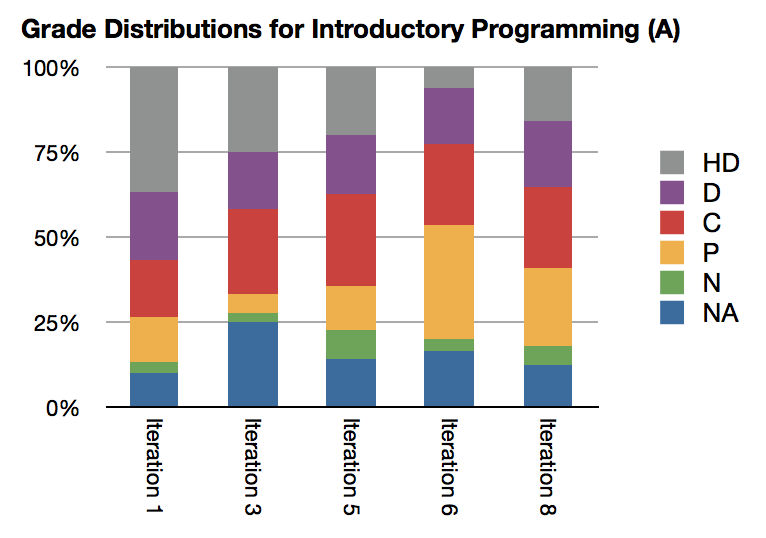
\includegraphics[width=0.8\columnwidth]{IntroProgA}
  \caption{Result distributions for Introductory Programming (A) from Iterations 1, 3, 5, 6 and 8.}
  \label{fig:intro_prog_1_9}
\end{figure}

\fref{fig:oop_1_9} shows the grade distributions for Object Oriented Programming (A). In Iteration 2 the pass rate was 69\%; this improved in Iteration 4 to 74\%. The percentage of students achieving Distinction and High Distinction dropped over this time from 29\% to 26\% in Iteration 4.

\begin{figure}[htbp]
  \centering
  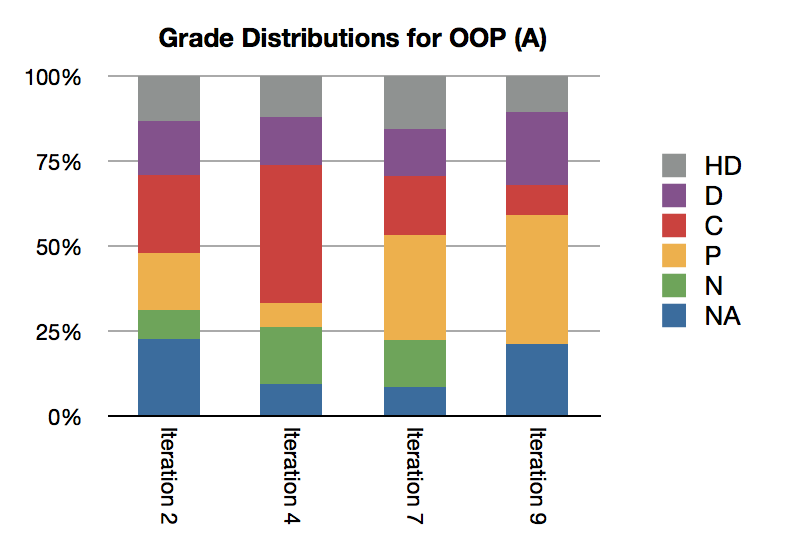
\includegraphics[width=0.8\columnwidth]{OOPA}
  \caption{Result distributions for Object Oriented Programming (A) from Iterations 2, 4, 7 and 9.}
  \label{fig:oop_1_9}
\end{figure}

% \begin{figure}[htbp]
%   \centering
%   \includegraphics[width=\columnwidth]{Iterations3to5}
%   \caption{Result distributions from Iterations 3 to 5.}
%   \label{fig:iterations_3_6}
% \end{figure}

% subsubsection data (end)

\paragraph{Reflections and Analysis} % (fold)

Staff reflections from these teaching periods indicated the improvements with the assessment criteria had helped reduce the time needed to perform the portfolio assessment, and this improved with each iteration. In terms of student learning, the lost productivity from Iteration 2 was not present in these iterations and student portfolios demonstrated continually improving outcomes. We believe this can be attributed to our developing experience with portfolio assessment, the improvements in the clarity of the assessment criteria, and the availability of prior portfolios as examples of what was required.

With these iterations we finally felt we were making progress and starting to receive the benefits we had hoped this teaching environment may achieve. Staff felt that student outcomes better match their expectations, and that the quality of student work improved each semester as better guidance was provided.

\paragraph{Development of Principles} % (fold)

The environment created in Iterations 3 to 6 had aimed to address the issues identified in Iteration 2, and then worked on improving the assessment criteria and available resources. At the end of these iterations it was felt that the portfolio had been an effective means of assessing student outcomes.

By the end of Iteration 6, it was apparent that the separation of assessment criteria by intended learning outcome was overly confusing, and had not productive for either staff or students aiming for higher grades. The criteria to meet the \emph{Outstanding} standard had required students to create a program of their own design. To achieve this, students had to apply their understanding of the concepts covered by the unit, but the assessment criteria had then required separate documentation for each intended learning outcome. This was time consuming for the students to prepare and for staff to assess. At the same time the separation of these reports made it difficult for students to demonstrate how the different aspects of the unit related to each other.

This experience influenced a number of the principles from \cref{cha:guiding_principles}. 

\begin{itemize}[noitemsep,nolistsep]
	\item The model had demonstrated an effective combination of constructive learning theories, \pref{itm:construct}, and aligned curriculum, \pref{itm:align}.
	\item Clearly communicating high expectations, \pref{itm:expectations}, had helped with the Theory Y environment, \pref{itm:theory_y}, and the focus on formative feedback, \pref{itm:formative}.
	\item The use of a reflective component in the portfolios, which relates to \pref{itm:reflect}, had been positive, and helped students to evaluate what they had learnt.
	\item Improvements in both how we taught and what we taught was greatly aided by reflective practice, \pref{itm:reflect}, and the focus on creating a productive learning environment \pref{itm:agile}.
	\item The separation of the assessment criteria by intended learning outcome had negatively impacted on students ability to demonstrate depth of knowledge, working against \pref{itm:depth}.
\end{itemize}

% paragraph development_of_principles (end)


% subsubsection iterations_3_to_6 (end)

% subsection as_the_model_stabilised (end)

\subsection{Latest Iterations} % (fold)
\label{sub:latest_iterations}

Iterations 3 to 6 had started to demonstrate the benefits of the portfolio assessment. Over these iterations the unit had been delivered to students enrolled in a degree with a focus on computer science. At the start of Iteration 7 the university was looking to consolidate programming units, and it was decided to trial the portfolio assessment approach with engineering students, in Introductory Programming (B). As so, these iterations aimed to continue to develop the model while also testing it with a wider range of students.

\begin{enumerate}[noitemsep,nolistsep]
	\item Iteration 7: Introductory Programming (B) was taught using the C programming language.
	\item Iteration 8: The two introductory programming units were combined into a single unit. This used two programming languages, starting with Pascal and then moving to C later in the semester.
	\item Iteration 9: Combined together the two object oriented programming units. Prior to this iteration Object Oriented Programming (B) had been taught using a textbook style approach, focusing on language syntax, and was assessed using assignments and a final exam.
\end{enumerate}

\subsubsection{Iterations 7, 8, and 9} % (fold)
\label{sub:iterations_7_to_9}

\paragraph{Focus} % (fold)

The focus for iterations 7 to 9 was on expressing assessment criteria that required a consolidation of knowledge across the unit's intended learning outcome. Higher grades would require the application of the unit's intended learning outcomes in the development of a project of the students own design. 

The second focus of these iterations was the incorporation of other units into this approach: Introductory Programming (B) and Object Oriented Programming (B). This increased the number of students to which this approach was delivered, and broadened the cohort to include students not necessarily interested in software development.

\paragraph{Action Plan} % (fold)

For these iterations the assessment criteria was as shown in \fref{fig:assessment_criteria}. This was accompanied by an explanation of what was required from the individual components: weekly tasks, tests, own program, and research report. For the assessment criteria, the main challenge in iterations 7 to 9 had been on trying to find clear requirements for the Credit grade. This needed students to demonstrate good coverage of the intended learning outcomes, while limiting the required workload. The following list shows what was used as the criteria for the Credit grade over these iterations.

\begin{itemize}[noitemsep,nolistsep]
  \item Iteration 7: Students were required to complete a piece of their own creation that demonstrated good coverage of all intended learning outcomes. The Unit Outline suggested that this could include reports, concept maps, glossaries, or any other piece the student wanted to create.
  \item Iteration 8 and 9: Weekly tasks included core tasks, and extension tasks. The core tasks included strong guidance, whereas the extension tasks required a greater level of independence. The Credit grade required all weekly tasks to be completed, as well as a selection of the weekly extension tasks. This also kept the other piece of the students own creation as in Iteration 7. \fref{fig:i9_assessment_criteria} shows an example of the assessment criteria from Introductory Programming (B) in Iteration 9.
\end{itemize}

In terms of teaching and learning resources, these iterations included the redevelopment of a number of resources, and the development of the task tracking system.

\begin{enumerate}[noitemsep,nolistsep]
  \item Iteration 7: 
  \begin{itemize}[noitemsep,nolistsep]
  	\item A new version of the Programming Arcana was created, this version used SwinGame, focused on procedures first and the C programming language.
  	\item SwinGame was used from week 1 in core lab tasks, enabling the procedures first approach.
  	\item Syntax diagrams created for the Programming Arcana were used in the Lecture slides.
  	\item Weekly exercises were moved into the Programming Arcana.
  	\item The Introductory Programming video podcasts were created to support the lecture material.
  \end{itemize}

  \item Iteration 8:
  \begin{itemize}[noitemsep,nolistsep]
  	\item The new Programming Arcana was extended to include both the C and Pascal programming languages.
  	\item Weekly exercises were moved back into the laboratory handout.
  	\item Additional documentation was provided to demonstrate the research process, and how a small research project could be conducted and documented.
  \end{itemize}

  \item Iteration 9:
  \begin{itemize}[noitemsep,nolistsep]
  	\item Weekly exercises were adjusted to include Lab exercises, Core exercises, and Extension exercises. The Lab exercises were designed to be worked through in the laboratory class under the guidance of the tutor. These exercises did not need to be included in student portfolios.
  	\item The Doubtfire tool was developed, and Core exercises were used as the weekly tasks for the burn down charts. To be eligible for Credit students needed to have all Core exercises signed off.
  \end{itemize}
\end{enumerate}


% subsubsection plan (end)

\paragraph{Data} % (fold)

For software development students the pass rate continued to rise through these iterations, with 82\% of students passing Introductory Programming (A) and 79\% passing Object Oriented Programming (A) in Iteration 9.

In Iteration 7, Introductory Programming (B) was introduced and achieved a 71\% pass rate. However, student portfolios were generally considered to be weaker than for those in Introductory Programming (A) and fewer students achieved high grades. This can also be seen in \fref{fig:combined}, which shows the results for the combined units in iterations 8 and 9.

\begin{figure}[htbp]
  \centering
  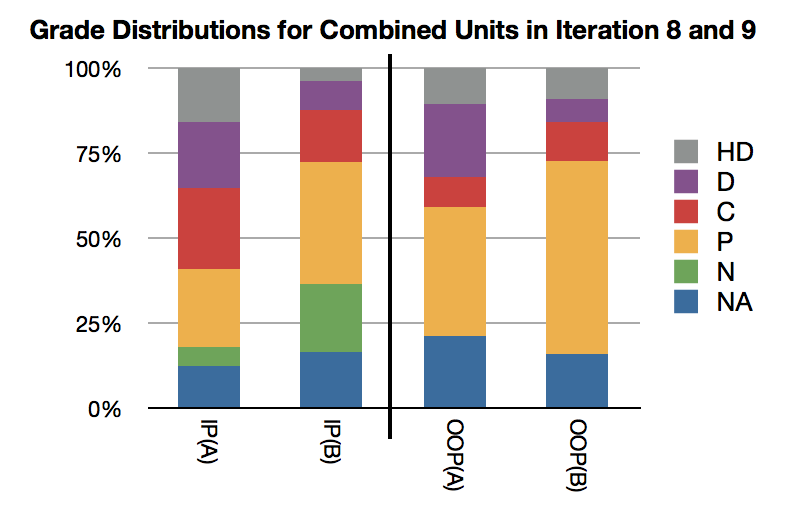
\includegraphics[width=0.8\textwidth]{CombinedUnits}
  \caption{Result distributions for combined units in iterations 8 and 9.}
  \label{fig:combined}
\end{figure}

\paragraph{Reflections and Analysis} % (fold)

With Introductory Programming (A) the quality of submitted portfolios continued to improve through these iterations. In Iteration 8 extra guidance was provided on how to conduct and document a small research project, and this seems to have been beneficial with an increased number of High Distinction portfolios.

With the other cohorts, the results seem less positive. Staff indicated a difficulty in engaging students not enrolled in a degree that focused on software development. This was most pronounced in the combined introductory programming unit, as can be seen in \fref{fig:combined}. Given that both groups of students had been delivered the same material, in the same classes, it had been assumed that the distribution of results should be similar. A one-way ANOVA was used to test for differences in results amongst the different student cohorts. Results from the units differed significantly across the two cohorts, F (1, 219) = 28.94, p = 0.0000. These results are discussed further in \sref{sec:evaluating_progress_using_burndown_charts}.

\begin{figure}[htbp]
  \centering
  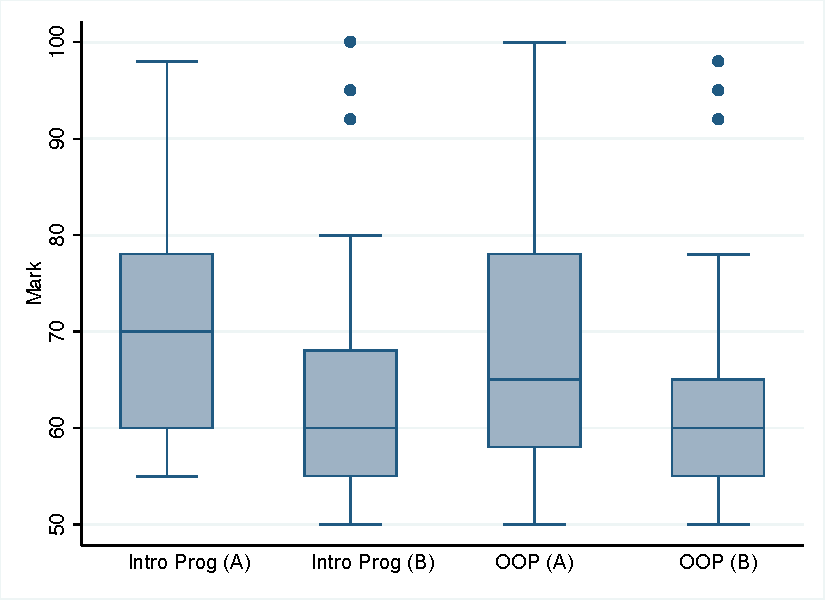
\includegraphics[width=0.8\textwidth]{CombinedUnitsBox}
  \caption{A box plot showing the distribution of results across the two combined units}
  \label{fig:combined_box}
\end{figure}

The clarity of the assessment criteria and the clear delineation of what is required for the Pass, Distinction and High Distinction grades further reduced the time needed to assess the portfolios.

While staff felt that the portfolio assessment was very successful through these iterations, the criteria for the Credit grade remained unclear and tended to require students to complete \emph{more work} rather than demonstrate \emph{better understanding}.

\paragraph{Development of Principles} % (fold)

These iterations followed the model described in \cref{cha:approach}, and delivered the units as outlined in \cref{cha:example_impl}. The implementations across these iterations embodied all of the principles from \cref{cha:guiding_principles}. The focus on creating a productive learning environment and reflection, a combination of \pref{itm:agile} and \pref{itm:reflect}, continued to ensure that the process improved in each iteration.

% subsection iterations_7_to_9 (end)

% subsection latest_iterations (end)

\subsection{Current Iteration} % (fold)

\paragraph{Focus}
This teaching approach is currently being used to deliver Iteration 10. In this iteration the focus is on achieving better outcomes in the combined units, and to reduce the workload required by the Credit criteria while still maintaining the same standard.

\paragraph{Plan}
One of the success stories from Iteration 9 was the use of a Glossary covering programming terminology, abstractions, and statements. This was used as a means of getting students to \emph{describe} and \emph{explain} principles and associated concepts, and seemed to be an effective means of both engaging the students with the material and assessing their learning outcomes. As a result, Iteration 10 will use the glossary for the Credit criteria. It is hoped this will help students engage appropriately with the teaching and learning activities.

% subsection  (end)

\subsection{Summary} % (fold)
\label{sub:action_summary}

This section has presented results and analysis from nine iterations of an action research project that examined the implementation of portfolio assessment. The overall focus of this work was on development, application, and ongoing evaluation of the model from \cref{cha:approach}.

Initial attempts at portfolio assessment failed to appropriately capture staff expectation, and student portfolios were generally weaker than desired. Over subsequent iterations, the assessment criteria evolved to more tightly define what was expected of each grade and students portfolios improved to meet these expectations. In the final iterations, staff were able to quickly assess portfolios, and felt that grades accurately reflected student outcomes.

This work provides additional evidence of the strength of portfolio assessments for achieving constructive alignment. In each iteration the assessment criteria helped guide students in preparing their portfolios, and as the criteria evolved the evidence in student portfolios improved. Experience delivering portfolio assessed units resulted in criteria that clearly relates to active verbs at the multi-structural and relational levels of the SOLO taxonomy.

Our experience highlights the importance of ensuring intended learning outcomes are expressed clearly, and capture the core concepts and principles that need to be demonstrated in student portfolios. The assessment criteria then maps the intended learning outcomes to statements of required levels of achievement. Together the intended learning outcomes and assessment criteria express what needs to be done and how well it needs to be done to achieve different grades.

The model presented in \cref{cha:approach} provided an effective means of achieving constructive alignment. For students, the process provides support and encouragement through iterative formative feedback, gives them clear expectations of what they need to achieve, and results in meaningful grades. After an initial investment, the intended learning outcomes and assessment criteria provide a dual means for staff to express expectations, and the resulting environment encouraged reflective practice. During the teaching period, staff and student efforts are both directed toward the one goal: helping students achieve the intended learning outcomes to the best of their ability.

% subsection discussion (end)

% section lessions_learnt_from_action_research (end)
\clearpage
\section{Issues Identified in Student Reflections} % (fold)
\label{sec:issues_identified_in_student_reflections}

Student reflections provide an open opportunity to identify issues that are relevant from the students' perspective. The investigation presented in this section analyses issues identified in student reflections from the Introductory Programming (A) unit in Iteration 6, and we provide some recommendations to help inform the development of units using this approach. 


\subsection{Method} % (fold)
\label{sub:issues_method}

This section is divided into three parts to clearly describe the details of \emph{Introductory Programming (A) in Iteration 6}, the \emph{Student Cohort and Research Participation}, and the \emph{Thematic Analysis of Reflections}. In the Introductory Programming Unit section we provide details of the unit that was investigated as part of this research. The Student Cohort and Research Participation section details the student body undertaking this unit and how they were recruited to be part of this research. Finally the Thematic Analysis of Reflections section outlines the process followed to extract and analyse the data from the student portfolios.

\subsubsection{Introductory Programming (A) in Iteration 6} % (fold)
\label{sub:intro_prog_i6}

In Iteration 6, Introductory Programming (A) had implemented the large majority of the principles and processed discussed in \cref{cha:guiding_principles} and \cref{cha:approach}. The teaching and learning activities differed slightly from the introductory programming unit described in \cref{cha:example_impl}, though the emphasis on concepts over syntax was present. The topics for the twelve lectures for this teaching period are shown in the following list.
\begin{enumerate}[noitemsep,nolistsep]
  \item Programs, Procedure, Compiling and Syntax
  \item User Input and Working with Data
  \item Functions, Procedures, and Parameters
  \item Branches and Loops
  \item Custom Data Types
  \item Functional Decomposition
  \item Case Study
  \item Pointers and Dynamic Memory Management
  \item Structured Programming
  \item Recursion and Backtracking
  \item Portfolio Preparation
  \item Review and Future Studies
\end{enumerate}

The unit's delivery included an early introduction topic of ``understanding syntax'', where students were taught how to read programming language syntax using the visual ``railroad'' diagram syntax notation. This allowed later lecture topics to focus on concepts, with syntax being offloaded to programming demonstrations and supplied notes, which included railroad diagrams and small code examples for each programming statement.

As described in \cref{cha:example_impl}, the allocated classes were designed with the goal of actively engaging students. Lectures typically included a review of previous topics, a short presentation using ``Beyond Bullet Points'' style lecture slides, an interactive programming demonstration, and group activities. Laboratory sessions involved code reading activities, guided coding activities, and practical hands-on exercises.

The approach to assessment included weekly submissions and formative feedback to help students develop their understanding, three hurdle tests to ensure basic competence, and portfolio assessment for final grades.

Students were asked to reflect on their learning in the Learning Summary Report, and a template document was provided to assist students in preparing their comments. The template prompted students to describe the pieces they had included, to describe how these related to the unit's intended learning outcomes, and then to reflect on what they had learnt from the unit.

To help students in writing their reflections, the following instructions were provided in the template. 
\begin{quote}
  \small
  Think about what you have learnt in this unit, and reflect on what you think were key learning points or incidents. Answer questions such as: What did you learn? What do you think was important? What did you find interesting? What have you learnt that will be valuable for you in the future? Which activities helped you most? Has this changed the way you think about software development? Did you learn what you wanted/expected to learn? Did you make effective use of your time? How could you improve your approach to learning in the future? Etc. 
\end{quote}

Note that there were no prompts for students to include details on issues they had encountered, meaning that any issues expressed should have been significant to the learning experience of the student.

\subsubsection{Student Cohort and Research Participation} % (fold)
\label{sub:issues_student_cohort}

In Iteration 6 the Introductory Programming (A) unit was undertaken by 84 students, 70 of whom submitted a portfolio for assessment. Participation in the research was voluntary, with informed consent being sought in lecture 11 as outlined in \sref{sub:addressing_ethical_concerns}.

\tref{tbl:issues_student_numbers} shows the number of portfolios made available to this research, the number that included comments related to the theme of ``issues'' and the distribution of grades. The grade distribution is also shown in \fref{fig:issues_grade_dist}, and will be discussed in \sref{sec:issues_discussion}.

\begin{table*}[p]
	\footnotesize
	\renewcommand{\arraystretch}{1.3}
	\caption{Portfolios submitted, issue comments and grade distribution.}
	\label{tbl:issues_student_numbers}
	\centering
	\begin{tabular}{l|c|c|c|c|c|c}
    % \hline
        ~                     & Total & HD & D & C & P & F  \\ \hline
        Submitted Portfolio   & 70    & 5                & 14          & 20     & 28   & 3     \\ % \hline
        Agreed to participate & 59    & 5                & 13          & 16     & 23   & 2     \\ % \hline
        Commented on Issues   & 35    & 2                & 6           & 11     & 14   & 2     \\ 
         - Learning Issues    & 26    & 2                & 3           & 9     & 12   & 1     \\ 
         - Programming Issues & 22    & 1                & 4           & 8     & 7   & 2     \\
		%\hline
	\end{tabular}
\end{table*}

\begin{figure}[thbp]
	\centering
	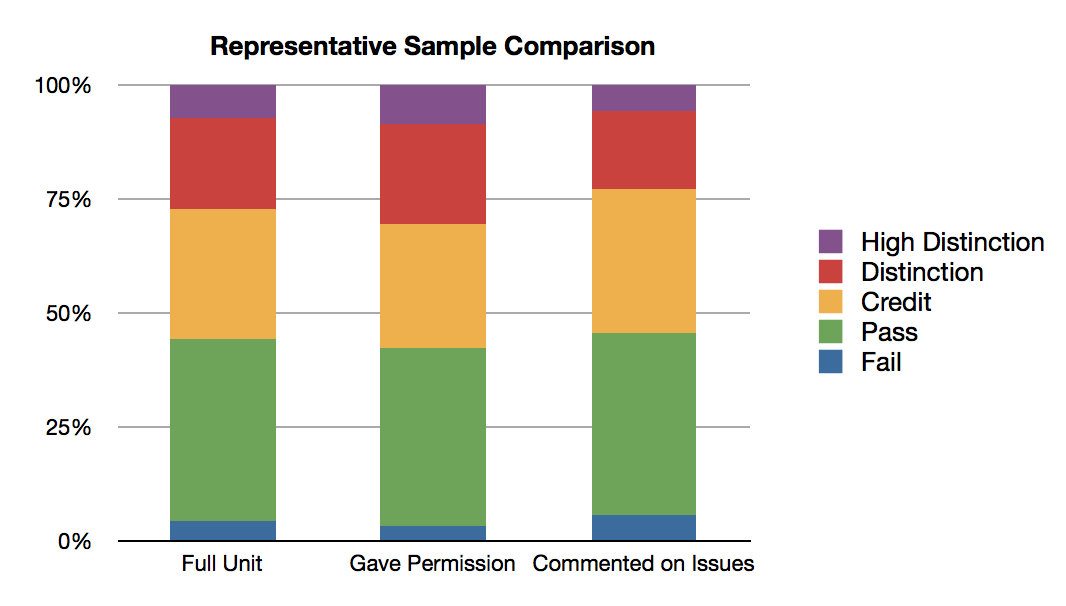
\includegraphics[width=0.8\textwidth]{IssuesGradeDistributions}
	\caption{Distribution of grades for the full unit, for those students who agreed to participate in the research, and for those who commented on issues.}
	\label{fig:issues_grade_dist}
\end{figure}



% subsection student_cohort (end)
% subsection introductory_programming (end)

\subsubsection{Thematic Analysis of Reflections} % (fold)
\label{sub:thematic_analysis_of_reflections}

The thematic analysis of student reflections followed the process outlined in \sref{sub:thematic_analysis}. Initial themes were generated by examining the reflective component of each portfolio and looking for all explicit mention of issues the student faced. Each new issue identified was matched to a theme and recorded in a spreadsheet. To ensure that all issues were reported in the results, the process of grouping themes did not remove or ignore any issues raised. All issues that could not be grouped into an existing theme were collected together as a miscellaneous ``other'' theme. The Results section outlines the different themes identified, and how these themes relate to the comments raised by students in their reflections.

% subsection thematic_analysis_of_reflections (end)
% section method (end)

\subsection{Results} % (fold)
\label{sec:issues_results}

A number of themes emerged from the analysis, and can be broadly classified as either general \emph{learning issues} or \emph{programming related issues}. (See \tref{tbl:issues_student_numbers} and \fref{fig:student_numbers}.) Each of these categories is presented in \tref{tbl:theme_counts} along with the number of students who raised these issues, broken down by grade. The following sections describe the individual themes in more detail.

\begin{table}[htbp]
	  \footnotesize
	  \renewcommand{\arraystretch}{1.3}
	
	\caption{Issue count results for grade and theme. Values of interest are indicated using bold format.}
	\label{tbl:theme_counts}
	\centering
	
    \begin{tabular}{l|p{5cm}|c|c|c|c|c|c}
    % \hline
        Theme                  & Description & Total & HD & D & C  & P  & F \\ \hline \hline
        Learning Issues        & Issues related to learning in general.           & ~    & ~  & ~ & ~ & ~ & ~ \\ %\hline
        - Time Issues            & Time constraints, or issues with time management.           & 14    & 1  & 0 & \textbf{5}  & \textbf{8}  & 0 \\ %\hline
        - Getting Started        & Comments relating to initial weeks, or tacking early hurdles.            & 8     & 0  & 1 & 2  & \textbf{5}  & 0 \\ %\hline
        - Learn through mistakes & Specifically commented on having issues and learning from these.           & 7     & 1  & 2 & 2  & 2  & 0 \\ %\hline
        - Other                  & Other learning related concepts not allocated to other themes.           & 5     & 0  & 0 & 2  & 2  & 1 \\ %\hline
        Totals        & ~           & ~    & 2  & 3 & 11 & 17 & 1 \\ \hline % \hline
        Programming Issues     & Issues related to programming topics, or technical areas.           & ~    & ~  & ~ & ~ & ~ & ~ \\ %\hline
        - Pointers               & Use of pointers and dynamic memory allocation functions.            & 11    & 1  & 2 & \textbf{4}  & 3  & 1 \\ %\hline
        - Parameters             & Mentions parameters, or parameter passing           & 8     & 0  & 1 & \textbf{4}  & 3  & 0 \\ %\hline
        - Program Design         & Algorithm and program structure design           & 7     & 0  & 1 & 1  & 3  & 2 \\ %\hline
        - Other (Syntax)           & Other issues, but related to the language syntax or concepts.           & 7    & 0  & 0 & 2  & 3  & 2 \\ %\hline
        - Other (General)                  & Other programming issues not allocated to other themes.           & 5    & 0  & 0 & 2  & 2  & 1 \\ %\hline
        - Recursion              & Declaration and use of recursive functions or data structures.           & 4    & 0  & 1 & 2  & 1  & 0 \\ %\hline
        Totals     & ~           & ~    & 1  & 4 & 14 & 11 & 3 \\ % \hline
        
    % \hline
	\end{tabular}	
\end{table}

\begin{figure}[thbp]
	\centering
	\includegraphics[width=0.8\textwidth]{NumStudentsMentioningIssues}
	\caption{Number of students mentioning learning issues and programming issues.  See \tref{tbl:issues_student_numbers}.}
	\label{fig:student_numbers}
\end{figure}

%TODO: SP noted that this is very info heavy. Still... i like it. :)

\subsubsection{General Learning Issues} % (fold)
\label{sub:general_learning_issues}

The \emph{general learning issues} capture all of the comments made by students that do not relate directly to a given programming topic or technical aspect of the unit, but instead relate to the students' learning experience in general. In this category the themes that appeared include  \emph{time management},  \emph{getting started} with the unit, and \emph{learning through mistakes}. The issue counts and grade distribution of these are included in \tref{tbl:theme_counts}, and can also be seen in \fref{fig:learning_issues}.

\emph{Time management issues} identified in the students' reflections included comments about aspects such as ``staying on task'', wishing they had ``asked for help earlier'', or the general need to improve their time management to enable them to achieve higher grades. It can be seen that the majority of these concerns were raised by students who obtained either a Pass or Credit grade. These comments are further supported by observations from teaching staff, who noted concerns about students not working consistently through the semester and not seeking help in a timely manner.

The next largest general learning issue was \emph{getting started} with programming. These comments specifically indicated issues related to the initial hurdle of getting started with the unit. One student noted this as their first experience using a computer, while others commented on the difficulty of the first few weeks' lab exercises. Again, these findings are supported by observations from the teaching staff who noted that a number of students withdraw from the unit before census date,\footnote{This is the date when the university records enrolment numbers, typically a few weeks after the start of the semester to allow for changes of enrolment.} and there was a general drop in enrolment numbers around this time. This may indicate that a larger number of students faced these issues but did not continue with the unit, though further work is needed to verify this.

%% !!!! NOTE:  !!!! Not really an issue... how can we keep this in? I think it's important

The last main issue in this section related to students reflecting on the mistakes or struggles that provided them with an opportunity to learn something important, referred to as \emph{learning through mistakes}. For example, one student's reflection noted that:

\begin{quote}
``\ldots I suddenly gained insight [into the code] I had been struggling with \ldots''
\end{quote}

\noindent The reflection continued on to comment that having overcoming these issues the student gained a clearer understanding of the concepts taught up to that point, and that subsequent programs were easier to understand. 

A number of \emph{other} issues were identified by individual students. These issues included: 
\begin{itemize}[noitemsep,nolistsep]
	\item transitioning to university life and study,
	\item finding information in the online learning management system,
	\item seeking help in general,
	\item keeping up with the pace of the unit, noted as ``challenging but good'', and
	\item adjusting to portfolio assessment.
\end{itemize}
%TODO: added the "noted in one example" ... as the quote was unsupported. Hmm?

% subsection general_learning_issues (end)

\begin{figure}[htbp]
	\centering
	\includegraphics[width=0.9\textwidth]{LearningIssues}
	\caption{Number of students mentioning issues related to learning. See \tref{tbl:theme_counts}.}
	\label{fig:learning_issues}
\end{figure}


\subsubsection{Programming Issues} % (fold)
\label{sub:programming_issues}

As already mentioned, fewer students commented on programming or technical issues in their reflections than the more general learning issues. The programming sub-themes matched specific topics covered in the unit, including \emph{pointers}, \emph{parameters}, \emph{program design}, and \emph{recursion}. In this theme the \emph{other} sub-theme featured more prominently, with a larger range of issues being located in the reflections of only one or two students. The data for these themes is listed in \tref{tbl:theme_counts} and shown in \fref{fig:programming_issues}.

\begin{figure}[htbp]
	\centering
	\includegraphics[width=0.9\textwidth]{ProgrammingIssues}
	\caption{Number of students mentioning issues related to programming. See \tref{tbl:theme_counts}.}
	\label{fig:programming_issues}
\end{figure}

Amongst the identified programming issues, \emph{pointers} featured most prominently. Comments typically just referred to having issues with ``pointers'', with the more detailed comments discussing issues with knowing when to dereference pointers and being unsure of when to use pointers. This is further supported by notes from teaching staff indicating that pointers tended to be problematic even for students who demonstrated strong programming skills up to this point in the material.

\emph{Parameters} were also mentioned by a number of students as being a topic that was particularly challenging. This included comments relating to tracing parameter values through a number of function or procedure calls, and issues of a single value having different names across different routines. From these comments there is a direct connection from parameter issues to a student's understanding of program structure, or more importantly execution flow.

Issues relating to \emph{Program Design} were also raised in the portfolio reflections. These comments related to aspects such as using functional decomposition, planning program structure, and designing algorithms.

The \textbf{other} issues for the programming category captures issues identified by one or two students. These were classified as relating either to \textbf{syntax and concepts} or \textbf{general programming} issues, and were:

\begin{itemize}[noitemsep,nolistsep]
  \item Syntax issues included:
  \begin{itemize}[noitemsep,nolistsep]
    \item iteration and working with loops,
    \item using arrays (two comments),
    \item creating composite data types using records,
    \item functions in general,
    \item dealing with syntax errors, and 
    \item using units to divide programs into multiple files.
  \end{itemize}
  \item General programming issues included:
  \begin{itemize}[noitemsep,nolistsep]
    \item ``Programming in general'',
    \item ``Following program code'' in code reading exercises,
    \item difficulties finding and using resources from the SwinGame library, and
    \item the maths needed to achieve programming tasks.
  \end{itemize}
\end{itemize}

There were also a number of reflections that raised the topic of \textbf{recursion}; these mentioned issues with both recursive functions and data structures. 

% subsection programming_issues (end)
% section results (end)

\subsection{Discussion} % (fold)
\label{sec:issues_discussion}

\subsubsection{Investigation Focus and Sample Quality}
% context
Comments provided by students, when reflecting on their learning during any unit, can be valuable and interesting in many ways, especially with respect to the evaluation of a particular approach to teaching. Our investigation focused specifically on the theme of issues mentioned or identified by students in their reflective reports. Results of the thematic analysis, presented in Section \ref{sec:issues_results}, identified clear key themes. Additionally, several individual comments were selected.

% The quality of the data - good 
The analysis considered a sample of reflective reports presented in a single semester unit. Of the 70 students in the class, almost 85\% were willing to participate. Within the participant group, 35 students wrote one or more comments that matched the target theme. \tref{tbl:issues_student_numbers} and \fref{fig:issues_grade_dist} show that the relative distribution of grades in the contributing group matches closely to both the participant group and the entire results for the unit. This strongly supports that the results are a representative sample of the unit, at least with respect to grade distribution. 

% Is is possible that the sample is not representative of students who like to keep to themselves and tend to communicate less.

\subsubsection{General Learning Versus Programming Issues} % (fold)
\label{sub:balance_of_learning_versus_programming_issues}

Beginning with the two key themes of general learning issues and programming issues (\tref{tbl:issues_student_numbers} and \fref{fig:student_numbers}) it can been seen that the distribution of student grades is very similar, with a slightly stronger representation of Pass students in the learning issues theme.

Overall, more students commented on learning in general. This is of particular interest given the relative emphasis of the course material, which focuses on teaching programming concepts over syntax details. Despite the relatively small time spent on syntax, students did not mention having related issues.

A closer examination of the issues related to programming strengthens this analysis further. Most student comments on programming issues (\tref{tbl:theme_counts}) concerned applying programming concepts, rather than issues of understanding syntax. Also, these comments were about when and how to use the related programming concepts rather than specifically how to apply the syntax of the language used. 

Comparison of the grade distributions within the learning issues (\fref{fig:learning_issues}) and programming issues (\fref{fig:programming_issues}) suggests potentially interesting differences, such as issues specific to grade groups, and other issues across all grades. The sample size of this investigation limits any significant insight although some points are listed in later discussion.

% subsection balance_of_learning_versus_programming_issues (end)

\subsubsection{Learning Issues}

\paragraph{Time Management} % (fold)
\label{ssub:time_management}

Time management issues were identified by the largest number of students (\tref{tbl:theme_counts}). The grade distribution is skewed towards student's who achieved Pass and Credit results (bold values), suggesting that students who do achieve Distinction or High Distinction results managed time better, and that the unit structure requires good time management to achieve these outcomes.

Developing a portfolio that demonstrates the ability to apply concepts taught requires time: time to practice using the concepts, and time to demonstrate their use competently. For students to achieve Distinction and High Distinction grades, they need to be able to organise their time effectively. 

With more traditional forms of assessment, marks can be used as incentives. Using assessment due dates during the delivery of the unit has the effect of turning marks into time distributed weighted incentives. Marks no longer represent the importance of the learning outcome, but match allocation of incentive. Consider, for example, the allocation of marks for lab attendance. These marks do not help measure the students' learning outcomes, but are purely there to incentivise lab attendance. Similarly, assignments due within the unit delivery period assess the speed of acquiring the required knowledge. 

With portfolio assessment the summative assessment is delayed until after unit delivery. This has the benefit of providing a more direct assessment of learning outcomes, but has a cost related to loss of incentives during delivery. While this is positive from a learning perspective, it can easily lead to students delaying their work on portfolio assessed units in order to address the more time critical assignments in other units. Given the number of comments related to this issue, it appears to be easy for students to then lose sight of how they are falling behind in a unit with a relatively flexible portfolio assessment.

% subsubsection time_management (end)

\paragraph{Getting Started} % (fold)
\label{ssub:getting_started}

Getting started is another issue facing many students (\tref{tbl:theme_counts} and \fref{fig:learning_issues}). In the first few weeks of the semester, students will face practical and conceptual issues. Practical issues include installing compilers and text editors, learning to use command line tools, and issues with general computer use. At the same time students need to build a viable conceptual model of computing \cite{Hoc:1990}, and relate this to the programs they are creating. 

Early on students may also face challenges transitioning to university study and university life in general. In the first few weeks students are also more likely to have issues with syntax, and dealing with syntax errors. Together these challenges can present a significant hurdle for students.

These issues could be addressed in a number of ways. Shifting toward an IDE could remove some issues related to the use of the command line compiler, but add overhead related to use of a more complex programming environment, and do not assist students in building their conceptual model of computing. The teaching staff also felt that students undertaking this unit do need to learn to use the command line, and this early introduction meant that later units could expect at least some familiarity with command line tools.

% subsubsection getting_started (end)

\paragraph{Learning Through Mistakes} % (fold)
\label{ssub:learning_through_mistakes}
%  - - learning through mistakes (constructivism) across all grade levels (suggestive)

The students' active role in building their own conceptual model of a topic plays a significant role in constructive learning theories \cite{Glasersfeld:1989}. Effective teaching then becomes the ability to place students in situations where errors in their understanding can be challenged to help the students build viable conceptual models. 

With this in mind, it is interesting to note, as shown in \tref{tbl:theme_counts}, the number of students who commented on gaining significant understanding through making mistakes. In line with constructive thinking, these students encountered situations in which their conceptual model was inappropriate, and in addressing the associated problems they were able to gain a better, more robust, conceptual model.

Comments about learning through mistakes were distributed across all grades, from Pass through to High Distinction (\fref{fig:learning_issues}). This suggests that mistake-based learning experiences are beneficial to a wide range of students, albeit with some gaining a better understanding than others through the process. 

% subsubsection learning_through_mistakes (end)


\paragraph{Other Learning Issues} % (fold)
\label{ssub:other_learning_issues}

From the other issues students noted, many can be attributed to transitioning to university education. Learning to locate and use learning resources and to seek help, are all issues that students must come to deal with when shifting to university education.

It is interesting to note that one student did raise a complaint about portfolio assessment, indicating that it would be easier to sit an exam. While this is only a single student, it does highlight that the purpose of the ongoing assessment may not be realised by all. \citet{Tang:1999} indicated that students tend to apply narrower learning strategies for examinations, focusing on memorising material covered in lectures. In contrast, \citet{Tang:1999} found that with portfolio assessment students adopted a wider perspective, making use of higher cognitive activities such as application, relation, and reflection. Students are likely to find these higher cognitive activities more challenging, and therefore those who wish to apply surface learning approaches are likely to prefer other assessment strategies.

% subsubsection other_learning_issues (end)

\subsubsection{Programming Issues}

\paragraph{Pointers and Recursion} % (fold)
\label{ssub:pointers_and_recursion}

Our results support those from \citet{Lahtinen:2005} in indicating that students find learning pointers challenging. Issues related to using pointers and memory management featured across a range of grade results (\tref{tbl:theme_counts} and \fref{fig:programming_issues}), indicating that this concept was challenging even for those students who managed to achieve good results in the unit. 

Pointers require a good conceptual understanding of computing, and the ability to debug logical errors. Issues with pointers can often result in abrupt program termination, which can be very confronting for beginner programmers. Locating the cause of these errors is an additional challenge, that requires a students to build a mental model of what is happening within the programs they have written.

Issues with recursion were raised by fewer students than other issues, which is in contrast to the study by \citet{Lahtinen:2005}. This may be explained by the short time students had with recursion in this study. A deep exploration of recursion was not required for students to pass the unit. It is likely, therefore, that many students may not have had sufficient time to explore more complex applications of recursion.

In addition to being complex, pointers and recursion both occur relatively late in the curriculum. With pointers, students had little time to develop the skills necessary to handle associated issues, whereas with recursion the short time meant students had little opportunity to develop programs of sufficient complexity to encounter issues.  In either case, at the time of writing their reflections, issues with later lecture topics are perhaps more likely to be in focus.

% subsubsection pointers_and_recursion (end)

% From the comments ... identified the following themes.
%  - Technical
% Programming General - pointers and parameters (minor recursion, arrays)

\paragraph{Parameters} % (fold)
\label{ssub:parameters}

Parameters require students to understand local scoping of variables, procedure and function calls, and methods for sharing these values between functions and procedures. This appears to be another point at which students need to expand their model of computing \cite{Hoc:1990}. 

While parameter concepts can take time to understand, issues are likely to be constructive in nature. When the logic for a program is contained within a single procedure, students can develop a simplistic model of what is occurring when other functions or procedures are called. When students need to design their own functions and procedures that require parameters, they are presented with situations that challenge their simplistic model. This suggests that parameters provide a significant learning opportunity from a constructive perspective.

The two different parameter passing methods are both taught in the unit, with pass by reference being used to create procedures to swap parameter values, as well as allowing procedures to modify data within structures and arrays. Call by reference provides an early introduction to references. 
% Make point on parameters (link to research), suggests turning point in learning (link to constructivism), occurs early (week 3), suggests enabling concept


% subsubsection parameters (end)


\paragraph{Program and Algorithm Design} % (fold)
\label{ssub:program_and_algorithm_design}

Program and algorithm design are progressively taught throughout the unit, with the main focus being in the middle of the unit's delivery in topics related to functional decomposition and structured programming. Comments by students indicated several issues on how to practically apply the concepts covered to create programs. 

We initially expected a larger representation of this issue, as design tasks require a deeper, relational, understanding of the concepts being used. However, the core tasks students had to submit for a Pass grade were accompanied with detailed instructions to help ease these design issues. Extension tasks required for a Credit grade did require some design components, and less guidance was provided. Students attempting their own program, necessary for a Distinction grade, needed to perform design activities as these programs were of their own design and creation.

% subsubsection program_and_algorithm_design (end)

\paragraph{Other Programming Issues} % (fold)
\label{ssub:other_programming_issues}

The other programming issues raised by students can be classified as individual challenges. It seems that students are likely to learn at different paces, in different ways, and find different topics challenging. Again, general comments concerned the application of programming concepts, rather than with programming language syntax. Each of the raised issues indicated a point at which students had an opportunity to challenge and develop their conceptual understanding of programming and their model of computing. 

% subsubsection other_programming_issues (end)

\subsubsection{Recommendations}
 
Based on the thematic results and on the experiences of staff involved in the unit delivery, there are a number of implications and recommendations that can be made. These recommendations are listed below, and will be explained in later sections:

\begin{itemize}[noitemsep,nolistsep]
	\item strongly avoid mixing formative with summative assessment,
	\item give students time to adjust to portfolio assessment, 
	\item focus on student ``awareness'',
	\item use a quick formative feedback process, 
	\item avoid the ``tutor debugging'' phenomena,  
	\item use visual methods to convey progress, and  
	\item make students aware of issues they are likely to face.
	% \item the SwinGame API risk/benefit...
	% \item (TODO) how help those who don't ask (who are they?)
\end{itemize}

\paragraph{Always formative, lastly summative}

Separating formative feedback processes from summative marking has a clear value, and this is reflected in student comments. Our observation is that using a punitive marking system creates an incentive for students to hide faults and limits in their understanding. Students need to know what they need to learn. Related to this is the time a student can spend asking about marking schemes or lost marks -- time better spent on learning.

% It takes time...
\paragraph{Students need time to adjust}

In comments to staff, students have said that it takes time to get used to a portfolio based unit even if they understand the principles. If we consider that students might be conditioned to respond to summative marking and due dates as a way of allocating their attention, an interesting question emerges: how do we help students maintain an active engagement with the unit activities? The Doubtfire tool was one attempt at answering this question, though this remains an ongoing challenge and research opportunity.
 
\paragraph{Focus on student awareness}
 
Primarily, student awareness is the basis for positive engagement and an aware student has the opportunity to make appropriate choices. To support this, staff need to communicate the structure, activities and expectations of a portfolio-based unit to students as effectively as possible. Unfortunately students may essentially have habits that can take time to adjust. It is possible to help students with issues such as time management and, hence, learning outcomes.

Although formative activities many not have due date or marks (grade penalties), staff should still express clear expectations of when work needs to be done. In some cases this leverages a students' habits to their advantage as they feel compelled to do the work. Ideally, students should give these formative tasks as high a priority as assignments with marks.

\paragraph{Use quick formative feedback}

Very quick feedback helps to create strong reinforcement in a student that the process really is formative and personally valuable. In a students' experience summative marking is often a delayed process. If formative feedback takes a long time it is removed from the students' current learning and challenges, and so can be confused as summative marking. Students need to be engaged with the formative nature of these assessments, making use of the feedback to help develop their understanding.

\paragraph{Avoid tutor debugging}

A possible problem with quick formative feedback, and resubmission opportunities, is that students may submit poorly prepared ``drafts'' and use staff simply to ``fix things''. This issue has been described as ``tutor debugging'' by some of our staff, and should be actively discouraged. One approach to this is to set minimum submission standards for work submitted for feedback. 

\paragraph{Use visual methods to convey progress }

Visual charting of tasks and completed work, calendar events and strong reminders of work and time limitations help to engage students. It is also possible that a ``gamefication'' approach, by recognising personal or group achievements and rewarding with awards, ``badges'' an other game-related concepts, can create a fun and personal incentive for students. We also recognise that there are also risks with gamefication, such as trivialisation of the value of core learning activities or distorting the value of learning activities through association to a gamefication artefact.

\paragraph{Tell students what to expect}
Finally, helping students understand the issues they are likely to face should help them prepare sufficiently for the more challenging tasks. This is particularly relevant to the issues related to getting started. The challenges early on in the unit may put a number of students off, and these students are likely to lose motivation and engagement with the unit. Making them aware that these challenges are ``normal'', and to be expected, may assist them in getting over early hurdles.

% section discussion (end)

\subsection{Summary} % (fold)
\label{sub:issues_summary}

In this section we have presented a thematic analysis of reflective reports presented by students as part of their assessment in the Introductory Programming (A) unit. The development and delivery of the unit followed the model from \cref{cha:approach}, being an implementation of the introductory programming unit described in \cref{cha:example_impl}. A good representation of students distributed across all result grades agreed to participate in the study. 

Thematic analysis was directed specifically at the theme of \emph{issues} identified by students. Overall results showed that more students raised learning issues than programming related issues. Significant learning themes included time management, getting started and mistake-based learning. The most common programming issues were related to pointers and parameters, with only a small number of issues related to syntax, and both these results were expected. Issues related to program design were raised less than expected. 

The discussion considered a number of interesting results, and put forward recommendations and future directions for research in this area. 

% subsection summary (end)

% section issues_identified_in_student_reflections (end)

\clearpage
\section{Evaluating Progress using Burn Down Charts} % (fold)
\label{sec:evaluating_progress_using_burndown_charts}

The work presented in this section examines the rate of student progress, as recorded using the Doubtfire task tracking tool and reported in student portfolio. By examining the various rates of progress and grades associated with these portfolios, we are able to provide some insights into the teaching and learning environment and recommendations to help inform the development of units using this approach. 

% Structure of Paper

% The following sections first outline the method used in conducting this research, providing details on the teaching and learning context, student cohort, method used for the analysis, and a brief overview of the online task tracking system. This is followed by the results from the data collection phase, and then the Discussion presents our interpretation and analysis of the data.

% section evaluating_progress_using_burndown_charts (end)


\subsection{Method} % (fold)
\label{sec:progress_method}

As with \sref{sub:issues_method}, this section is divided into three parts with the aim of clearly describing the teaching and learning context, the student cohort, and the details for the thematic analysis.

\subsubsection{Teaching and Learning Context} % (fold)
\label{sub:progress_teaching_and_learning_context}

This work analysed the progress of students from Introductory Programming (B) in Iteration 9. In Iteration 9, the teaching period consisted of thirteen weeks, twelve of which were teaching weeks, and a single week semester break in week six. Topics for the twelve lectures are shown in the following list.

\begin{enumerate}[noitemsep,nolistsep]
  \item Programs, Procedure, Compiling and Syntax
  \item User Input and Working with Data
  \item Control Flow: Branches and Loops
  \item Procedural and Structured Programming
  \item Arrays
  \item Custom Data Types
  \item Pointers and Dynamic Memory Management
  \item Learning a New Language  (C)
  \item Portfolio Discussion
  \item Arrays and Structures in C, and Recursion
  \item Pointers in C, and Backtracking
  \item Review and Future Studies
\end{enumerate}

An overview of the assessment criteria for Introductory Programming (B) in Iteration 9 is shown in \fref{fig:i9_assessment_criteria}. To be eligible for a pass grade students include a range of work of the weekly assessment tasks, and indicated how the pieces included demonstrated coverage of all intended learning outcomes. For Credit, student needed to complete all weekly assignments and include pieces that demonstrated good coverage of all intended learning outcomes. Distinction and High Distinction grades required students to go beyond these weekly tasks. Distinction grades were awarded for being able to apply the concepts learnt in the development a program designed by the student. High Distinction required students to undertake a small research project, and write this up in a short research report.

\begin{figure}[htbp]
  \centering
  \includegraphics[width=\textwidth]{AssessmentCriteria}
  \caption{Overview of assessment criteria provided to students in the unit outline.}
  \label{fig:i9_assessment_criteria}
\end{figure}

In Iteration 9, the Doubtfire tool was used to track student progress against the Core Tasks from the weekly exercises. An example of the charts from Introductory Programming (B) in Iteration 9 is shown in \fref{fig:progress_example_chart}. As described in \cref{cha:supporting}, the charts shown the cumulative amount of work remaining week by week, which decreases as work is completed. 

\begin{figure}[thbp]
  \centering
  \includegraphics[width=0.8\textwidth]{ExampleChart}
  \caption{An example burn down chart showing progress against weekly tasks for Introductory Programming (B) in Iteration 9.}
  \label{fig:progress_example_chart} 
\end{figure}

% subsubsection use_of_doubtfire_in_the_unit (end)

\subsubsection{Student Cohort and Research Participation} % (fold)
\label{sub:progress_student_cohort}

At the end of the teaching period 139 students submitted portfolios for assessment. Of these, 87 agreed to participate in this research. Participation in the research was voluntary, with informed consent being sought using the process described in \sref{sub:addressing_ethical_concerns} in lecture 9.

\tref{tbl:progress_student_numbers} shows the grade distribution of the submitted portfolios, those made available to this research and of these, those who included their burn down chart in their portfolio.

\begin{table}[hbp]
  \footnotesize
  \renewcommand{\arraystretch}{1.3}
  \caption{Grade distribution of portfolios submitted.}
  \label{tbl:progress_student_numbers}
  \centering
  \begin{tabular}{l|c|c|c|c|c|c}
    % \hline
        ~                     & Total & HD & D & C & P & N  \\ \hline
        Submitted Portfolio   & 139    & 7                & 25          & 24     & 79   & 4     \\ % \hline
        Agreed to participate & 87    & 6                & 22          & 17     & 39   & 3     \\ % \hline
        Included Chart & 80 & 6 & 22 & 17 & 33 & 2 \\
    %\hline
  \end{tabular}
\end{table}

\begin{figure}[thbp]
  \centering
  \includegraphics[width=0.7\textwidth]{ProgressGradeDistributions}
  \caption{Distribution of grades for the full unit, for those students who agreed to participate in the research, and those who included the burndown chart.}
  \label{fig:progress_grade_dist}
\end{figure}

% subsection sub:progress_student_cohort (end)

\subsubsection{Thematic Analysis to Identify Trends in Progress} % (fold)
\label{sub:approach_to_analysis}

The process from \sref{sub:thematic_analysis} was used in order to identify the themes and patterns associated with student progress. To gaining familiarisation with the data, the burn down charts from each portfolio were scanned and combined into a single document. Each page of the resulting document included the chart and a code to identify the portfolio from whence it came. To ease the process of visual classification the charts were scaled to similar size. The resulting document was then printed and each page was examined in order to determine appropriate classifications. 

Charts were classified based on the separation between the \textbf{Target Completion} line, which represented the target due dates, and the \textbf{Actual Completion} line, which indicated student progress based on the work having been signed off as complete by their Tutor. This process resulted in a number of chart classifications, and subclasses. Once the charts were classified they were examined again for any common features that occurred across classifications. 

% subsection approach_to_analysis (end)

\subsection{Results} % (fold)
\label{sec:progress_results}

\subsubsection{Identifed Chart Classifications} % (fold)
\label{sub:identified_chart_classifications}

Analysis of the charts made available to this research identified seven different classification related to the distance between the actual and target completion lines.Each classification is described in the following list, and illustrated in \fref{fig:chart_types}.

\begin{enumerate}[noitemsep,nolistsep]
  \item Tight trend with little diversion from the target completion line (Class \textbf{A}).
  \item Close to line and similar to Class A but with more deviation, though never more than one to two weeks delay before returning to the target completion line (Class \textbf{B}).
  \item Consistently trending down, but with sustained small gap(s) from the target completion line (Class \textbf{C}).
  \item Primarily off the target completion line, with occasional (rare) points where work caught up with the schedule (Class \textbf{D}). 
  \item More distant from the line, but catching up toward the end of the unit (Class \textbf{E}).
  \item Mostly distant from the line, with progress made in large steps (Class \textbf{F}).
  \item Not complete, chart included but student was not able to get all work signed off (Class \textbf{N}).
\end{enumerate}

\begin{figure}[p]
  \centering
  \includegraphics[width=0.71\textwidth]{CharTypes}
  \caption{Illustrations of the seven chart classifications identified in this work. The thicker blue line represents the Target Completion line, the thinner orange line the Actual Completion.}
  \label{fig:chart_types}
\end{figure}

\tref{tbl:chart_numbers} shows the frequency of each chart class in the analysed portfolios, and their associated grade distributions. The pie chart in \fref{fig:chart_dist} shows the distribution of the classifications, with the highlighted section indicating the number of students who did not get all tasks signed off (Class N).

\begin{table}[htbp]
  \footnotesize
  \renewcommand{\arraystretch}{1.3}
  \caption{Chart classification numbers, and grade distribution.}
  \label{tbl:chart_numbers}
  \centering
    \begin{tabular}{l|c|c|c|c|c|c}
        Class & Total & N & P  & C & D & HD \\ \hline
        A     & 7     & 0 & 0  & 0 & 6 & 1  \\ 
        B     & 7     & 0 & 0  & 4 & 1 & 2  \\ 
        C     & 10    & 0 & 1  & 3 & 5 & 1  \\ 
        D     & 9     & 0 & 2  & 5 & 2 & 0  \\ 
        E     & 6     & 0 & 1  & 2 & 3 & 0  \\ 
        F     & 9     & 0 & 1  & 2 & 4 & 2  \\ 
        N     & 32    & 2 & 28 & 1 & 1 & 0  
    \end{tabular}
\end{table}

\begin{figure}[thb]
  \centering
  \includegraphics[width=0.55\textwidth]{DistributionOfChartClassifications}
  \caption{Distribution of portfolios according to chart class. Note that 40\% of students did not have all weekly tasks signed off.}
  \label{fig:chart_dist}
\end{figure}

% subsection primary_chart_categories (end)

\subsubsection{Chart Features and Subclasses} % (fold)
\label{sub:chart_subclasses}

% Most of the chart classifications presented a number of interesting features or identifiable subclasses.

Five of the seven Class A charts demonstrated cases where students got ahead of the scheduled work. This was also evident in five of the seven Class B charts, and three Class C charts. Of special interest are the two students with Class D charts, more distant from the target completion line, who also managed to get ahead. A total of fifteen students were able to get ahead at some stage, and in all cases this occurred around week nine, after the shift to the C programming language. 

Two subclasses were evident in the Class C charts, as illustrated in \fref{fig:c_subclass}. The first subclass included a consistent gap from the scheduled line. This subclass constantly trended down, but did not rejoin the scheduled line during the semester. The second subclass exhibited a jagged shape with constant gaps coming back to the scheduled line at regular intervals. Interestingly none of the second subclass got ahead at any stage. Both subgroups consisted of five charts.

\begin{figure}[htbp]
  \centering
  \includegraphics[width=0.9\textwidth]{ChartCSubclass}
  \caption{Illustrations of the two Class C subclasses.}
  \label{fig:c_subclass}
\end{figure}

The Class D charts had two identified subclasses, as illustrated in \fref{fig:d_subclass}. The larger subclass, subclass 1, had ``golf club'' shaped charts with effort at the end after a long period without progress (a flat line). The second subclass was characterised by a slow start, but catching up to the target completion line around the middle of the semester. The first subclass consisted of five charts, with four in the second subclass.

\begin{figure}[htbp]
  \centering
  \includegraphics[width=0.9\textwidth]{ChartDSubclass}
  \caption{Illustrations of the two Class D subclasses.}
  \label{fig:d_subclass}
\end{figure}

\fref{fig:f_subclass} illustrates the three subclasses that were identified for the charts most distant from the scheduled line (Class F). The subclasses included (1) three large steps to reach the end, (2) a plateau mid semester then progress toward the end, and (3) a similar ``golf club'' shape to Class D with a large amount of work being signed off at the end of the semester. 

\begin{figure}[htbp]
  \centering
  \includegraphics[width=0.9\textwidth]{ChartFSubclass}
  \caption{Illustrations of the three Class F subclasses.}
  \label{fig:f_subclass}
\end{figure}

Of the 32 students who did not get all weekly tasks signed off (Class N) 13 (41\%) had completed 75\% or more of the work by the end of the unit. A further 9 had completed more than 50\%, 8 had more than 25\%, with 2 having less than 25\% of the work signed off. This is shown in visually in \fref{fig:n_subclass}, with the pie chart in \fref{fig:end_point} illustrating the percentage of each of the end points. Two portfolios in Class N were awarded grades higher than pass as a result of special consideration.

\begin{figure}[htbp]
  \centering
  \includegraphics[width=0.9\textwidth]{ChartNSubclass}
  \caption{Illustrations of the different end points for Class N charts.}
  \label{fig:n_subclass}
\end{figure}

\begin{figure}[thbp]
  \centering
  \includegraphics[width=0.75\columnwidth]{AmountSignedOffForN}
  \caption{Percentage tasks signed off for students with Class N charts.}
  \label{fig:end_point}
\end{figure}

Of the other classes, most charts that were close to the line (Class B) had their deviation around week five, which coincided with the arrays topic. Whereas the group more distant from the line (Class E) typically had slow starts with strong finishes. 

% subsection chart_subcategories (end)



\subsubsection{Grades by Chart Classification} % (fold)
\label{sub:grades_by_chart_classification}

\tref{tbl:chart_numbers} includes the result distribution for each chart class, shown graphically in \fref{fig:grade_chart_dist}. Pass results were primarily from Class N, Credit results were distributed across classes B through F, Distinction across classes A through F, with High Distinctions coming from classes A though C and F.

\begin{figure}[thb]
  \centering
  \includegraphics[width=\columnwidth]{GradesForEachChartKind}
  \caption{Distribution of grades for each of the identified chart classes.}
  \label{fig:grade_chart_dist}
\end{figure}


% subsection grades_by_chart_classification (end)


% section results (end)


\subsection{Discussion} % (fold)
\label{sec:progress_discussion}

\subsubsection{Focus of Investigation, and Quality of Sample Used} % (fold)
\label{sub:focus_of_investigation_and_quality_of_sample_used}

% focus
Understanding how students progress through an introductory programming unit can provide valuable insight into the strategies they are using and the methodology underpinning the teaching and learning context. Our investigation examined burn down charts included in student portfolios, which captured the rate at which students were able to complete formative assessment tasks and have them signed off by their tutors.  Results of the thematic analysis, presented in Section \ref{sec:progress_results}, identified a number of different chart classes and presented details on associated result distributions.

% sample quality = good
The investigation examined a sample of the portfolios submitted in a single semester, with 80 (58\%) of the portfolios being included in the analysis. The distribution of grades for these groups are shown in \tref{tbl:progress_student_numbers} and \fref{fig:progress_grade_dist}. The relative distribution of grades in the group with charts is reasonably representative of the entire unit, though the pass grade is under represented. However, as the pass grade students tended to be clustered in Class N, it is likely that the sample captured the variations in general student progress across all grades.

% subsection focus_of_investigation_and_quality_of_sample_used (end)

\subsubsection{Participation in Formative Assessment} % (fold)
\label{sub:participation_in_formative_assessment}

A number of the charts indicate active student engagement with the formative assessment throughout the semester. This is evident in the chart classes A through C, D (subclass 2), E, and N (for those who completed between 75\% but less than 100\% of the scheduled tasks). This represented 47 (59\%) of the 80 charts, and in all cases the charts indicated ongoing progress, which was only possible by engaging with the formative process. 

Our interpretation of the charts from Class D Subclass 1, with its distinctive ``golf club'' shape, is that these students are likely to have their attention diverted mid-semester. A possible cause is that the due dates for first assignments in parallel, unrelated, units typically fall in this period. Alternatively, these students may have needed additional time to bring all of the concepts together before continuing on with the C programming language. In either case, toward the end of the unit these students were then able to get back on track, and possibly get ahead of schedule. It would be interesting for future work to examine the reflections of these students to verify these interpretations.

The large drops in the Class F charts may be evidence of confident students who only occasionally submit their work for assessment. This may explain the large portion of D and HD results in this group.

A cause for concern is the large number of Class N charts, particularly where less than 75\% of the formative tasks were completed. This group made up 30 (38\%) of the 80 portfolios examined. The unit teaching staff indicated, overwhelmingly, that a lack of student engagement had been of particular concern for the semester under analysis. These students had little interest in learning to program, and seem to have taken superficial approaches to learning. This is evidenced in the both the final results and number of students with Class N charts.

% subsection participation_in_formative_assessment (end)


\subsubsection{Progress, Grades, and Formative Assessment} % (fold)
\label{sub:progress_grades_and_formative_assessment}

In reflecting on the distribution of grades across the different chart classifications, we believe that students have been able to achieve good results using a number of different strategies. If this is compared with units that use summative assessment during the semester, students with charts in classes C through F are likely to have lost some marks early on, as they were behind the target completion line at various stages during the semester. With the portfolio approach, 50\% of these students were able to go on and achieve a Distinction or higher grade.

Of particular interest are the students with charts in class E, which was characterised by a slow start and a strong finish. These appear to be students who struggled with concepts initially but eventually gained sufficient mastery to quickly catch up later in the semester. It is interesting to note the large portion of these students who were subsequently able to achieve a Distinction result. Even with the slow start, these students were able to apply the concepts learnt to the creation of their own program. Had this been a traditional programming unit, using summative assessment during the semester, loss of marks early on  may have lead to them not receiving a grade that represented their final learning outcome. If these students lacked confidence, then this negative reinforcement may possibly discourage them from attempting to master the concepts, and reinforce any negative opinion they have of the field in general.

% subsection progress_grades_and_formative_assessment (end)

% B * Close to Line - also close matching but with slightly more deviation, but never more than one to two weeks delay. Those with a 2 week delay occurred around week 5 (arrays) - back on track at week 7. (4 of 7 - issues with arrays). Something has happened at this point, if this is related to content this may indicate issues with arrays in this group that then learned from their mistakes and were able to get back on track with sufficient feedback. - most of these dip under the line with the switch to C. (6 of 7)

\subsubsection{Concept Based Approach} % (fold)
\label{sub:use_of_multiple_languages}

The charts also provide evidence of the effectiveness of the concept-based approach used. A total of 15 (19\%) of the 80 charts showed students getting ahead of the schedule after the switch to the C programming language. This mostly consisted of students with charts in classes A and B, though it also includes several students in classes C and E. 

After the language change, tasks were concerned with expressing previously presented concepts in the C language. We propose that students who committed to understanding the underlying programming concepts, rather than focussing on the Pascal language itself, were able to exploit this understanding when introduced to C. Analysis of reflections in these portfolios may provide additional evidence to help verify this. 

% subsection use_of_multiple_languages (end)

\subsubsection{Reflecting on Programming Issues} % (fold)
\label{sub:relation_to_issues}

This work helps support two of the general learning issues, as identified in \sref{sec:issues_identified_in_student_reflections}, facing students: getting started, and learning through mistakes. Other than classes A and B, most of the student's progress appears to indicate that they had issues getting started. This is understandable, given the highly interrelated nature of the programming concepts presented in early weeks. The progress students showed later in the semester also demonstrates that students are able to make progress while learning through mistakes. 

In relation to time management - the number one issue identified in our previous work - further analysis of student reflections is needed to determine if the tool provided them with useful feedback and motivation to keep on track. That said, the tool was actively used and provided staff with useful information on student progress throughout the teaching period.

% subsection relation_to_issues (end)


% section discussion (end)

\subsection{Summary} % (fold)
\label{sec:progress_summary}

In this section we presented a thematic analysis of student progress as evidenced by burn down charts included in their final portfolios. Details of the unit, its delivery, assessment, and its use of burn down charts to track progress was described as a context for this work.  

Thematic analysis identified several different chart classes, based on the shape of the chart and its distance from the target completion line. These classes provided evidence of students' approach to learning, with most concentrating on language features rather than underlying programming concepts. The different classes also presented evidence that students struggle to get started with introductory programming, but that once concepts were mastered they were able to catch up and, in some cases, get ahead of schedule. Interestingly, the use of formative feedback resulted in students being able to achieve high grades even when they struggled initially.

% section conclusion (end)

% chapter lessons_learnt_through_action_research (end)
%!TEX root = Constructive Alignment for Introductory Programming.tex

\chapter{Discussion} % (fold)
\label{cha:discussion}

\section{Formative and Summative Assessment} % (fold)
\label{sec:formative_and_summative_assessment}

% section formative_and_summative_assessment (end)

\section{What is a Portfolio?} % (fold)
\label{sec:what_is_a_portfolio_}

Too vague... many report using portfolios but other than Biggs original work none have used it in the same way.


Mixed mode assessment - assignments + portfolio, portfolio + exam.
= mixed messages

% section what_is_a_portfolio_ (end)

\section{Rebellious Robert and Selfless Susan} % (fold)
\label{sec:rebellious_robert_and_selfless_susan}

Approach to learning to program requires understanding... Marton:2005 indicates that education systems are not focused on this and as a result neither do our students... so they fail.

Approach to learning is still the number one issue, portfolio appears to work well for intrinsically motivated students ... but not so well for those who want to avoid the work (no silver bullet)

% section rebellious_robert_and_selfless_susan (end)

\section{Engaging Students in Introductory Programming} % (fold)
\label{sec:engaging_students_in_introductory_programming}


\citet{Guzdial:2005} non-majors

% section engaging_students_in_introductory_programming (end)

\section{Resources} % (fold)
\label{sec:resources}

Short/specific podcasts had a longer life

Concept podcasts were not as successful... 

Separation of activities and resources? - successfull

% section resources (end)

% \subsection{Related work on general education principles} % (fold)
% \label{ssub:related_work_on_education_principles}

% %
% % JG - I am not sure about this section in terms of fit & content...
% %
% % Maybe could incorporate in the principles sections???
% %
% %


% In discussing how to improve undergraduate education, \citet{Chickering:1987} listed seven principles for good practice in undergraduate education. These are practices that:
% \begin{enumerate}[noitemsep,nolistsep]
% 	\item Encourages contact between students and faculty.
% 	\item Develops reciprocity and cooperation among students
% 	\item Encourages active learning
% 	\item Gives prompt feedback
% 	\item Emphasizes time on task
% 	\item Communicates high expectations
% 	\item Respects diverse talents and ways of learning
% \end{enumerate}

% The following list states how each of the principles from \citet{Chickering:1987} are integrated with the principles underlying this work. 
% \begin{itemize}[noitemsep,nolistsep]
% 	\item The strong emphasis on frequent formative feedback should be used to help encourage contact between students and faculty. (\Pref{itm:formative}, \Pref{itm:support})
% 	\item This same formative process should also be harnessed to encourage sharing and cooperation amongst students. (\Pref{itm:formative},\Pref{itm:support},\Pref{itm:theory_y})
% 	\item The central nature of the students in constructing their knowledge necessitates an approach that encourages active learning. (\Pref{itm:construct},\Pref{itm:theory_y})
% 	\item The formative feedback process needs to ensure that work is returned promptly to students, ensuring they receive the feedback while it is still relevant. (\Pref{itm:formative})
% 	\item Communicating high expectations is included directly in our principles. (\Pref{itm:expectations})
% 	\item Assessment and teaching and learning activities need to be flexible, enabling different styles of learning and to engage with students diverse talents. (\Pref{itm:support})
% \end{itemize}


\section{Future Work} % (fold)
\label{sec:future_work}

structured Literature review - interesting to note referencing in the field

% section future_work (end)

% chapter discussion (end)
%!TEX root = Constructive Alignment for Introductory Programming.tex

\chapter{Conclusion} % (fold)
\label{cha:conclusion}

% chapter conclusion (end)


\bibliography{SenteReferences}
\end{document}
